\documentclass[]{book}
\usepackage{lmodern}
\usepackage{amssymb,amsmath}
\usepackage{ifxetex,ifluatex}
\usepackage{fixltx2e} % provides \textsubscript
\ifnum 0\ifxetex 1\fi\ifluatex 1\fi=0 % if pdftex
  \usepackage[T1]{fontenc}
  \usepackage[utf8]{inputenc}
\else % if luatex or xelatex
  \ifxetex
    \usepackage{mathspec}
  \else
    \usepackage{fontspec}
  \fi
  \defaultfontfeatures{Ligatures=TeX,Scale=MatchLowercase}
\fi
% use upquote if available, for straight quotes in verbatim environments
\IfFileExists{upquote.sty}{\usepackage{upquote}}{}
% use microtype if available
\IfFileExists{microtype.sty}{%
\usepackage{microtype}
\UseMicrotypeSet[protrusion]{basicmath} % disable protrusion for tt fonts
}{}
\usepackage{hyperref}
\hypersetup{unicode=true,
            pdftitle={기초통계 개념정리},
            pdfauthor={김진섭},
            pdfborder={0 0 0},
            breaklinks=true}
\urlstyle{same}  % don't use monospace font for urls
\usepackage{natbib}
\bibliographystyle{plainnat}
\usepackage{longtable,booktabs}
\usepackage{graphicx,grffile}
\makeatletter
\def\maxwidth{\ifdim\Gin@nat@width>\linewidth\linewidth\else\Gin@nat@width\fi}
\def\maxheight{\ifdim\Gin@nat@height>\textheight\textheight\else\Gin@nat@height\fi}
\makeatother
% Scale images if necessary, so that they will not overflow the page
% margins by default, and it is still possible to overwrite the defaults
% using explicit options in \includegraphics[width, height, ...]{}
\setkeys{Gin}{width=\maxwidth,height=\maxheight,keepaspectratio}
\IfFileExists{parskip.sty}{%
\usepackage{parskip}
}{% else
\setlength{\parindent}{0pt}
\setlength{\parskip}{6pt plus 2pt minus 1pt}
}
\setlength{\emergencystretch}{3em}  % prevent overfull lines
\providecommand{\tightlist}{%
  \setlength{\itemsep}{0pt}\setlength{\parskip}{0pt}}
\setcounter{secnumdepth}{5}
% Redefines (sub)paragraphs to behave more like sections
\ifx\paragraph\undefined\else
\let\oldparagraph\paragraph
\renewcommand{\paragraph}[1]{\oldparagraph{#1}\mbox{}}
\fi
\ifx\subparagraph\undefined\else
\let\oldsubparagraph\subparagraph
\renewcommand{\subparagraph}[1]{\oldsubparagraph{#1}\mbox{}}
\fi

%%% Use protect on footnotes to avoid problems with footnotes in titles
\let\rmarkdownfootnote\footnote%
\def\footnote{\protect\rmarkdownfootnote}

%%% Change title format to be more compact
\usepackage{titling}

% Create subtitle command for use in maketitle
\providecommand{\subtitle}[1]{
  \posttitle{
    \begin{center}\large#1\end{center}
    }
}

\setlength{\droptitle}{-2em}

  \title{기초통계 개념정리}
    \pretitle{\vspace{\droptitle}\centering\huge}
  \posttitle{\par}
    \author{김진섭}
    \preauthor{\centering\large\emph}
  \postauthor{\par}
      \predate{\centering\large\emph}
  \postdate{\par}
    \date{2019-10-08}

\usepackage{booktabs}
\usepackage{kotex} 
\usepackage[doublespacing]{setspace}  
\usepackage{multirow}

\begin{document}
\maketitle

{
\setcounter{tocdepth}{1}
\tableofcontents
}
\hypertarget{prerequisites}{%
\chapter{Prerequisites}\label{prerequisites}}

This is a basic statistics book written by \textbf{Jinseob Kim}.

\hypertarget{uxd655uxb960probability-vs-uxac00uxb2a5uxb3c4likelihood}{%
\chapter{확률(Probability) vs 가능도(Likelihood)}\label{uxd655uxb960probability-vs-uxac00uxb2a5uxb3c4likelihood}}

\hypertarget{uxc2dcuxc791uxd558uxba74uxc11c}{%
\section{시작하면서}\label{uxc2dcuxc791uxd558uxba74uxc11c}}

본 챕터에서는 \textbf{가능도(Likelihood)} 가 무엇인지 직관적으로 이해하는 것을 목표로 한다. 가능도는 정규분포부터 회귀분석과 최신 인공지능 알고리즘에 이르기까지 통계학의 모든 부분에서 빠질 수 없는 개념인데, 이상하게도 의학 또는 보건학을 다루는 통계학 책에서는 이 개념을 잘 설명하지 않는다. 물론 통계 비전공자에게 설명하기 까다로운 개념임을 인정하며, 이번 기회에 \textbf{확률(Probability)}과 비교를 통해 엄밀한 정의는 아니더라도 대략적인 느낌은 파악하도록 하자. 마지막에는 \textbf{최대 가능도 추정량(Maximum Likelihood Estimator)}이 나오는데, 통계적 추론에서 중심극한정리와 더불어 가장 중요한 개념 중 하나이므로 반드시 이해하고 넘어가도록 하자.

\hypertarget{uxd655uxb960}{%
\section{확률}\label{uxd655uxb960}}

주사위를 예를 들어 보자. 주사위를 던져서 나올 수 있는 숫자는 1,2,3,4,5,6이고 각 숫자가 나올 확률은 \(\frac{1}{6}\)로 모두 같다. 동전 10번 던져서 앞면은 0\textasciitilde{}10번 나올 수 있으며 각각의 확률은 계산해 보면 각각 0.001, 0.01, 0.044, 0.117, 0.205, 0.246, 0.205, 0.117, 0.044, 0.01, 0.001 이다. 두 경우 모두 일어날 수 있는 사건이 6개, 11개로 정해져 있으며 각각에 대한 확률을 구할 수 있고 확률의 합은 1이 된다.

\begin{verbatim}
## Warning in grid.Call(C_textBounds, as.graphicsAnnot(x$label), x$x, x$y, :
## conversion failure on '확률' in 'mbcsToSbcs': dot substituted for <ed>
\end{verbatim}

\begin{verbatim}
## Warning in grid.Call(C_textBounds, as.graphicsAnnot(x$label), x$x, x$y, :
## conversion failure on '확률' in 'mbcsToSbcs': dot substituted for <99>
\end{verbatim}

\begin{verbatim}
## Warning in grid.Call(C_textBounds, as.graphicsAnnot(x$label), x$x, x$y, :
## conversion failure on '확률' in 'mbcsToSbcs': dot substituted for <95>
\end{verbatim}

\begin{verbatim}
## Warning in grid.Call(C_textBounds, as.graphicsAnnot(x$label), x$x, x$y, :
## conversion failure on '확률' in 'mbcsToSbcs': dot substituted for <eb>
\end{verbatim}

\begin{verbatim}
## Warning in grid.Call(C_textBounds, as.graphicsAnnot(x$label), x$x, x$y, :
## conversion failure on '확률' in 'mbcsToSbcs': dot substituted for <a5>
\end{verbatim}

\begin{verbatim}
## Warning in grid.Call(C_textBounds, as.graphicsAnnot(x$label), x$x, x$y, :
## conversion failure on '확률' in 'mbcsToSbcs': dot substituted for <a0>
\end{verbatim}

\begin{verbatim}
## Warning in grid.Call(C_textBounds, as.graphicsAnnot(x$label), x$x, x$y, :
## conversion failure on '확률' in 'mbcsToSbcs': dot substituted for <ed>
\end{verbatim}

\begin{verbatim}
## Warning in grid.Call(C_textBounds, as.graphicsAnnot(x$label), x$x, x$y, :
## conversion failure on '확률' in 'mbcsToSbcs': dot substituted for <99>
\end{verbatim}

\begin{verbatim}
## Warning in grid.Call(C_textBounds, as.graphicsAnnot(x$label), x$x, x$y, :
## conversion failure on '확률' in 'mbcsToSbcs': dot substituted for <95>
\end{verbatim}

\begin{verbatim}
## Warning in grid.Call(C_textBounds, as.graphicsAnnot(x$label), x$x, x$y, :
## conversion failure on '확률' in 'mbcsToSbcs': dot substituted for <eb>
\end{verbatim}

\begin{verbatim}
## Warning in grid.Call(C_textBounds, as.graphicsAnnot(x$label), x$x, x$y, :
## conversion failure on '확률' in 'mbcsToSbcs': dot substituted for <a5>
\end{verbatim}

\begin{verbatim}
## Warning in grid.Call(C_textBounds, as.graphicsAnnot(x$label), x$x, x$y, :
## conversion failure on '확률' in 'mbcsToSbcs': dot substituted for <a0>
\end{verbatim}

\begin{verbatim}
## Warning in grid.Call(C_textBounds, as.graphicsAnnot(x$label), x$x, x$y, :
## conversion failure on '주사위 던지기' in 'mbcsToSbcs': dot substituted for
## <ec>
\end{verbatim}

\begin{verbatim}
## Warning in grid.Call(C_textBounds, as.graphicsAnnot(x$label), x$x, x$y, :
## conversion failure on '주사위 던지기' in 'mbcsToSbcs': dot substituted for
## <a3>
\end{verbatim}

\begin{verbatim}
## Warning in grid.Call(C_textBounds, as.graphicsAnnot(x$label), x$x, x$y, :
## conversion failure on '주사위 던지기' in 'mbcsToSbcs': dot substituted for
## <bc>
\end{verbatim}

\begin{verbatim}
## Warning in grid.Call(C_textBounds, as.graphicsAnnot(x$label), x$x, x$y, :
## conversion failure on '주사위 던지기' in 'mbcsToSbcs': dot substituted for
## <ec>
\end{verbatim}

\begin{verbatim}
## Warning in grid.Call(C_textBounds, as.graphicsAnnot(x$label), x$x, x$y, :
## conversion failure on '주사위 던지기' in 'mbcsToSbcs': dot substituted for
## <82>
\end{verbatim}

\begin{verbatim}
## Warning in grid.Call(C_textBounds, as.graphicsAnnot(x$label), x$x, x$y, :
## conversion failure on '주사위 던지기' in 'mbcsToSbcs': dot substituted for
## <ac>
\end{verbatim}

\begin{verbatim}
## Warning in grid.Call(C_textBounds, as.graphicsAnnot(x$label), x$x, x$y, :
## conversion failure on '주사위 던지기' in 'mbcsToSbcs': dot substituted for
## <ec>
\end{verbatim}

\begin{verbatim}
## Warning in grid.Call(C_textBounds, as.graphicsAnnot(x$label), x$x, x$y, :
## conversion failure on '주사위 던지기' in 'mbcsToSbcs': dot substituted for
## <9c>
\end{verbatim}

\begin{verbatim}
## Warning in grid.Call(C_textBounds, as.graphicsAnnot(x$label), x$x, x$y, :
## conversion failure on '주사위 던지기' in 'mbcsToSbcs': dot substituted for
## <84>
\end{verbatim}

\begin{verbatim}
## Warning in grid.Call(C_textBounds, as.graphicsAnnot(x$label), x$x, x$y, :
## conversion failure on '주사위 던지기' in 'mbcsToSbcs': dot substituted for
## <eb>
\end{verbatim}

\begin{verbatim}
## Warning in grid.Call(C_textBounds, as.graphicsAnnot(x$label), x$x, x$y, :
## conversion failure on '주사위 던지기' in 'mbcsToSbcs': dot substituted for
## <8d>
\end{verbatim}

\begin{verbatim}
## Warning in grid.Call(C_textBounds, as.graphicsAnnot(x$label), x$x, x$y, :
## conversion failure on '주사위 던지기' in 'mbcsToSbcs': dot substituted for
## <98>
\end{verbatim}

\begin{verbatim}
## Warning in grid.Call(C_textBounds, as.graphicsAnnot(x$label), x$x, x$y, :
## conversion failure on '주사위 던지기' in 'mbcsToSbcs': dot substituted for
## <ec>
\end{verbatim}

\begin{verbatim}
## Warning in grid.Call(C_textBounds, as.graphicsAnnot(x$label), x$x, x$y, :
## conversion failure on '주사위 던지기' in 'mbcsToSbcs': dot substituted for
## <a7>
\end{verbatim}

\begin{verbatim}
## Warning in grid.Call(C_textBounds, as.graphicsAnnot(x$label), x$x, x$y, :
## conversion failure on '주사위 던지기' in 'mbcsToSbcs': dot substituted for
## <80>
\end{verbatim}

\begin{verbatim}
## Warning in grid.Call(C_textBounds, as.graphicsAnnot(x$label), x$x, x$y, :
## conversion failure on '주사위 던지기' in 'mbcsToSbcs': dot substituted for
## <ea>
\end{verbatim}

\begin{verbatim}
## Warning in grid.Call(C_textBounds, as.graphicsAnnot(x$label), x$x, x$y, :
## conversion failure on '주사위 던지기' in 'mbcsToSbcs': dot substituted for
## <b8>
\end{verbatim}

\begin{verbatim}
## Warning in grid.Call(C_textBounds, as.graphicsAnnot(x$label), x$x, x$y, :
## conversion failure on '주사위 던지기' in 'mbcsToSbcs': dot substituted for
## <b0>
\end{verbatim}

\begin{verbatim}
## Warning in grid.Call(C_textBounds, as.graphicsAnnot(x$label), x$x, x$y, :
## conversion failure on '주사위 던지기' in 'mbcsToSbcs': dot substituted for
## <ec>
\end{verbatim}

\begin{verbatim}
## Warning in grid.Call(C_textBounds, as.graphicsAnnot(x$label), x$x, x$y, :
## conversion failure on '주사위 던지기' in 'mbcsToSbcs': dot substituted for
## <a3>
\end{verbatim}

\begin{verbatim}
## Warning in grid.Call(C_textBounds, as.graphicsAnnot(x$label), x$x, x$y, :
## conversion failure on '주사위 던지기' in 'mbcsToSbcs': dot substituted for
## <bc>
\end{verbatim}

\begin{verbatim}
## Warning in grid.Call(C_textBounds, as.graphicsAnnot(x$label), x$x, x$y, :
## conversion failure on '주사위 던지기' in 'mbcsToSbcs': dot substituted for
## <ec>
\end{verbatim}

\begin{verbatim}
## Warning in grid.Call(C_textBounds, as.graphicsAnnot(x$label), x$x, x$y, :
## conversion failure on '주사위 던지기' in 'mbcsToSbcs': dot substituted for
## <82>
\end{verbatim}

\begin{verbatim}
## Warning in grid.Call(C_textBounds, as.graphicsAnnot(x$label), x$x, x$y, :
## conversion failure on '주사위 던지기' in 'mbcsToSbcs': dot substituted for
## <ac>
\end{verbatim}

\begin{verbatim}
## Warning in grid.Call(C_textBounds, as.graphicsAnnot(x$label), x$x, x$y, :
## conversion failure on '주사위 던지기' in 'mbcsToSbcs': dot substituted for
## <ec>
\end{verbatim}

\begin{verbatim}
## Warning in grid.Call(C_textBounds, as.graphicsAnnot(x$label), x$x, x$y, :
## conversion failure on '주사위 던지기' in 'mbcsToSbcs': dot substituted for
## <9c>
\end{verbatim}

\begin{verbatim}
## Warning in grid.Call(C_textBounds, as.graphicsAnnot(x$label), x$x, x$y, :
## conversion failure on '주사위 던지기' in 'mbcsToSbcs': dot substituted for
## <84>
\end{verbatim}

\begin{verbatim}
## Warning in grid.Call(C_textBounds, as.graphicsAnnot(x$label), x$x, x$y, :
## conversion failure on '주사위 던지기' in 'mbcsToSbcs': dot substituted for
## <eb>
\end{verbatim}

\begin{verbatim}
## Warning in grid.Call(C_textBounds, as.graphicsAnnot(x$label), x$x, x$y, :
## conversion failure on '주사위 던지기' in 'mbcsToSbcs': dot substituted for
## <8d>
\end{verbatim}

\begin{verbatim}
## Warning in grid.Call(C_textBounds, as.graphicsAnnot(x$label), x$x, x$y, :
## conversion failure on '주사위 던지기' in 'mbcsToSbcs': dot substituted for
## <98>
\end{verbatim}

\begin{verbatim}
## Warning in grid.Call(C_textBounds, as.graphicsAnnot(x$label), x$x, x$y, :
## conversion failure on '주사위 던지기' in 'mbcsToSbcs': dot substituted for
## <ec>
\end{verbatim}

\begin{verbatim}
## Warning in grid.Call(C_textBounds, as.graphicsAnnot(x$label), x$x, x$y, :
## conversion failure on '주사위 던지기' in 'mbcsToSbcs': dot substituted for
## <a7>
\end{verbatim}

\begin{verbatim}
## Warning in grid.Call(C_textBounds, as.graphicsAnnot(x$label), x$x, x$y, :
## conversion failure on '주사위 던지기' in 'mbcsToSbcs': dot substituted for
## <80>
\end{verbatim}

\begin{verbatim}
## Warning in grid.Call(C_textBounds, as.graphicsAnnot(x$label), x$x, x$y, :
## conversion failure on '주사위 던지기' in 'mbcsToSbcs': dot substituted for
## <ea>
\end{verbatim}

\begin{verbatim}
## Warning in grid.Call(C_textBounds, as.graphicsAnnot(x$label), x$x, x$y, :
## conversion failure on '주사위 던지기' in 'mbcsToSbcs': dot substituted for
## <b8>
\end{verbatim}

\begin{verbatim}
## Warning in grid.Call(C_textBounds, as.graphicsAnnot(x$label), x$x, x$y, :
## conversion failure on '주사위 던지기' in 'mbcsToSbcs': dot substituted for
## <b0>
\end{verbatim}

\begin{verbatim}
## Warning in grid.Call(C_textBounds, as.graphicsAnnot(x$label), x$x, x$y, :
## conversion failure on '주사위 눈' in 'mbcsToSbcs': dot substituted for <ec>
\end{verbatim}

\begin{verbatim}
## Warning in grid.Call(C_textBounds, as.graphicsAnnot(x$label), x$x, x$y, :
## conversion failure on '주사위 눈' in 'mbcsToSbcs': dot substituted for <a3>
\end{verbatim}

\begin{verbatim}
## Warning in grid.Call(C_textBounds, as.graphicsAnnot(x$label), x$x, x$y, :
## conversion failure on '주사위 눈' in 'mbcsToSbcs': dot substituted for <bc>
\end{verbatim}

\begin{verbatim}
## Warning in grid.Call(C_textBounds, as.graphicsAnnot(x$label), x$x, x$y, :
## conversion failure on '주사위 눈' in 'mbcsToSbcs': dot substituted for <ec>
\end{verbatim}

\begin{verbatim}
## Warning in grid.Call(C_textBounds, as.graphicsAnnot(x$label), x$x, x$y, :
## conversion failure on '주사위 눈' in 'mbcsToSbcs': dot substituted for <82>
\end{verbatim}

\begin{verbatim}
## Warning in grid.Call(C_textBounds, as.graphicsAnnot(x$label), x$x, x$y, :
## conversion failure on '주사위 눈' in 'mbcsToSbcs': dot substituted for <ac>
\end{verbatim}

\begin{verbatim}
## Warning in grid.Call(C_textBounds, as.graphicsAnnot(x$label), x$x, x$y, :
## conversion failure on '주사위 눈' in 'mbcsToSbcs': dot substituted for <ec>
\end{verbatim}

\begin{verbatim}
## Warning in grid.Call(C_textBounds, as.graphicsAnnot(x$label), x$x, x$y, :
## conversion failure on '주사위 눈' in 'mbcsToSbcs': dot substituted for <9c>
\end{verbatim}

\begin{verbatim}
## Warning in grid.Call(C_textBounds, as.graphicsAnnot(x$label), x$x, x$y, :
## conversion failure on '주사위 눈' in 'mbcsToSbcs': dot substituted for <84>
\end{verbatim}

\begin{verbatim}
## Warning in grid.Call(C_textBounds, as.graphicsAnnot(x$label), x$x, x$y, :
## conversion failure on '주사위 눈' in 'mbcsToSbcs': dot substituted for <eb>
\end{verbatim}

\begin{verbatim}
## Warning in grid.Call(C_textBounds, as.graphicsAnnot(x$label), x$x, x$y, :
## conversion failure on '주사위 눈' in 'mbcsToSbcs': dot substituted for <88>

## Warning in grid.Call(C_textBounds, as.graphicsAnnot(x$label), x$x, x$y, :
## conversion failure on '주사위 눈' in 'mbcsToSbcs': dot substituted for <88>
\end{verbatim}

\begin{verbatim}
## Warning in grid.Call(C_textBounds, as.graphicsAnnot(x$label), x$x, x$y, :
## conversion failure on '주사위 눈' in 'mbcsToSbcs': dot substituted for <ec>
\end{verbatim}

\begin{verbatim}
## Warning in grid.Call(C_textBounds, as.graphicsAnnot(x$label), x$x, x$y, :
## conversion failure on '주사위 눈' in 'mbcsToSbcs': dot substituted for <a3>
\end{verbatim}

\begin{verbatim}
## Warning in grid.Call(C_textBounds, as.graphicsAnnot(x$label), x$x, x$y, :
## conversion failure on '주사위 눈' in 'mbcsToSbcs': dot substituted for <bc>
\end{verbatim}

\begin{verbatim}
## Warning in grid.Call(C_textBounds, as.graphicsAnnot(x$label), x$x, x$y, :
## conversion failure on '주사위 눈' in 'mbcsToSbcs': dot substituted for <ec>
\end{verbatim}

\begin{verbatim}
## Warning in grid.Call(C_textBounds, as.graphicsAnnot(x$label), x$x, x$y, :
## conversion failure on '주사위 눈' in 'mbcsToSbcs': dot substituted for <82>
\end{verbatim}

\begin{verbatim}
## Warning in grid.Call(C_textBounds, as.graphicsAnnot(x$label), x$x, x$y, :
## conversion failure on '주사위 눈' in 'mbcsToSbcs': dot substituted for <ac>
\end{verbatim}

\begin{verbatim}
## Warning in grid.Call(C_textBounds, as.graphicsAnnot(x$label), x$x, x$y, :
## conversion failure on '주사위 눈' in 'mbcsToSbcs': dot substituted for <ec>
\end{verbatim}

\begin{verbatim}
## Warning in grid.Call(C_textBounds, as.graphicsAnnot(x$label), x$x, x$y, :
## conversion failure on '주사위 눈' in 'mbcsToSbcs': dot substituted for <9c>
\end{verbatim}

\begin{verbatim}
## Warning in grid.Call(C_textBounds, as.graphicsAnnot(x$label), x$x, x$y, :
## conversion failure on '주사위 눈' in 'mbcsToSbcs': dot substituted for <84>
\end{verbatim}

\begin{verbatim}
## Warning in grid.Call(C_textBounds, as.graphicsAnnot(x$label), x$x, x$y, :
## conversion failure on '주사위 눈' in 'mbcsToSbcs': dot substituted for <eb>
\end{verbatim}

\begin{verbatim}
## Warning in grid.Call(C_textBounds, as.graphicsAnnot(x$label), x$x, x$y, :
## conversion failure on '주사위 눈' in 'mbcsToSbcs': dot substituted for <88>

## Warning in grid.Call(C_textBounds, as.graphicsAnnot(x$label), x$x, x$y, :
## conversion failure on '주사위 눈' in 'mbcsToSbcs': dot substituted for <88>
\end{verbatim}

\begin{verbatim}
## Warning in grid.Call(C_textBounds, as.graphicsAnnot(x$label), x$x, x$y, :
## conversion failure on '확률' in 'mbcsToSbcs': dot substituted for <ed>
\end{verbatim}

\begin{verbatim}
## Warning in grid.Call(C_textBounds, as.graphicsAnnot(x$label), x$x, x$y, :
## conversion failure on '확률' in 'mbcsToSbcs': dot substituted for <99>
\end{verbatim}

\begin{verbatim}
## Warning in grid.Call(C_textBounds, as.graphicsAnnot(x$label), x$x, x$y, :
## conversion failure on '확률' in 'mbcsToSbcs': dot substituted for <95>
\end{verbatim}

\begin{verbatim}
## Warning in grid.Call(C_textBounds, as.graphicsAnnot(x$label), x$x, x$y, :
## conversion failure on '확률' in 'mbcsToSbcs': dot substituted for <eb>
\end{verbatim}

\begin{verbatim}
## Warning in grid.Call(C_textBounds, as.graphicsAnnot(x$label), x$x, x$y, :
## conversion failure on '확률' in 'mbcsToSbcs': dot substituted for <a5>
\end{verbatim}

\begin{verbatim}
## Warning in grid.Call(C_textBounds, as.graphicsAnnot(x$label), x$x, x$y, :
## conversion failure on '확률' in 'mbcsToSbcs': dot substituted for <a0>
\end{verbatim}

\begin{verbatim}
## Warning in grid.Call(C_textBounds, as.graphicsAnnot(x$label), x$x, x$y, :
## conversion failure on '확률' in 'mbcsToSbcs': dot substituted for <ed>
\end{verbatim}

\begin{verbatim}
## Warning in grid.Call(C_textBounds, as.graphicsAnnot(x$label), x$x, x$y, :
## conversion failure on '확률' in 'mbcsToSbcs': dot substituted for <99>
\end{verbatim}

\begin{verbatim}
## Warning in grid.Call(C_textBounds, as.graphicsAnnot(x$label), x$x, x$y, :
## conversion failure on '확률' in 'mbcsToSbcs': dot substituted for <95>
\end{verbatim}

\begin{verbatim}
## Warning in grid.Call(C_textBounds, as.graphicsAnnot(x$label), x$x, x$y, :
## conversion failure on '확률' in 'mbcsToSbcs': dot substituted for <eb>
\end{verbatim}

\begin{verbatim}
## Warning in grid.Call(C_textBounds, as.graphicsAnnot(x$label), x$x, x$y, :
## conversion failure on '확률' in 'mbcsToSbcs': dot substituted for <a5>
\end{verbatim}

\begin{verbatim}
## Warning in grid.Call(C_textBounds, as.graphicsAnnot(x$label), x$x, x$y, :
## conversion failure on '확률' in 'mbcsToSbcs': dot substituted for <a0>
\end{verbatim}

\begin{verbatim}
## Warning in grid.Call(C_textBounds, as.graphicsAnnot(x$label), x$x, x$y, :
## conversion failure on '확률' in 'mbcsToSbcs': dot substituted for <ed>
\end{verbatim}

\begin{verbatim}
## Warning in grid.Call(C_textBounds, as.graphicsAnnot(x$label), x$x, x$y, :
## conversion failure on '확률' in 'mbcsToSbcs': dot substituted for <99>
\end{verbatim}

\begin{verbatim}
## Warning in grid.Call(C_textBounds, as.graphicsAnnot(x$label), x$x, x$y, :
## conversion failure on '확률' in 'mbcsToSbcs': dot substituted for <95>
\end{verbatim}

\begin{verbatim}
## Warning in grid.Call(C_textBounds, as.graphicsAnnot(x$label), x$x, x$y, :
## conversion failure on '확률' in 'mbcsToSbcs': dot substituted for <eb>
\end{verbatim}

\begin{verbatim}
## Warning in grid.Call(C_textBounds, as.graphicsAnnot(x$label), x$x, x$y, :
## conversion failure on '확률' in 'mbcsToSbcs': dot substituted for <a5>
\end{verbatim}

\begin{verbatim}
## Warning in grid.Call(C_textBounds, as.graphicsAnnot(x$label), x$x, x$y, :
## conversion failure on '확률' in 'mbcsToSbcs': dot substituted for <a0>
\end{verbatim}

\begin{verbatim}
## Warning in grid.Call(C_textBounds, as.graphicsAnnot(x$label), x$x, x$y, :
## conversion failure on '주사위 던지기' in 'mbcsToSbcs': dot substituted for
## <ec>
\end{verbatim}

\begin{verbatim}
## Warning in grid.Call(C_textBounds, as.graphicsAnnot(x$label), x$x, x$y, :
## conversion failure on '주사위 던지기' in 'mbcsToSbcs': dot substituted for
## <a3>
\end{verbatim}

\begin{verbatim}
## Warning in grid.Call(C_textBounds, as.graphicsAnnot(x$label), x$x, x$y, :
## conversion failure on '주사위 던지기' in 'mbcsToSbcs': dot substituted for
## <bc>
\end{verbatim}

\begin{verbatim}
## Warning in grid.Call(C_textBounds, as.graphicsAnnot(x$label), x$x, x$y, :
## conversion failure on '주사위 던지기' in 'mbcsToSbcs': dot substituted for
## <ec>
\end{verbatim}

\begin{verbatim}
## Warning in grid.Call(C_textBounds, as.graphicsAnnot(x$label), x$x, x$y, :
## conversion failure on '주사위 던지기' in 'mbcsToSbcs': dot substituted for
## <82>
\end{verbatim}

\begin{verbatim}
## Warning in grid.Call(C_textBounds, as.graphicsAnnot(x$label), x$x, x$y, :
## conversion failure on '주사위 던지기' in 'mbcsToSbcs': dot substituted for
## <ac>
\end{verbatim}

\begin{verbatim}
## Warning in grid.Call(C_textBounds, as.graphicsAnnot(x$label), x$x, x$y, :
## conversion failure on '주사위 던지기' in 'mbcsToSbcs': dot substituted for
## <ec>
\end{verbatim}

\begin{verbatim}
## Warning in grid.Call(C_textBounds, as.graphicsAnnot(x$label), x$x, x$y, :
## conversion failure on '주사위 던지기' in 'mbcsToSbcs': dot substituted for
## <9c>
\end{verbatim}

\begin{verbatim}
## Warning in grid.Call(C_textBounds, as.graphicsAnnot(x$label), x$x, x$y, :
## conversion failure on '주사위 던지기' in 'mbcsToSbcs': dot substituted for
## <84>
\end{verbatim}

\begin{verbatim}
## Warning in grid.Call(C_textBounds, as.graphicsAnnot(x$label), x$x, x$y, :
## conversion failure on '주사위 던지기' in 'mbcsToSbcs': dot substituted for
## <eb>
\end{verbatim}

\begin{verbatim}
## Warning in grid.Call(C_textBounds, as.graphicsAnnot(x$label), x$x, x$y, :
## conversion failure on '주사위 던지기' in 'mbcsToSbcs': dot substituted for
## <8d>
\end{verbatim}

\begin{verbatim}
## Warning in grid.Call(C_textBounds, as.graphicsAnnot(x$label), x$x, x$y, :
## conversion failure on '주사위 던지기' in 'mbcsToSbcs': dot substituted for
## <98>
\end{verbatim}

\begin{verbatim}
## Warning in grid.Call(C_textBounds, as.graphicsAnnot(x$label), x$x, x$y, :
## conversion failure on '주사위 던지기' in 'mbcsToSbcs': dot substituted for
## <ec>
\end{verbatim}

\begin{verbatim}
## Warning in grid.Call(C_textBounds, as.graphicsAnnot(x$label), x$x, x$y, :
## conversion failure on '주사위 던지기' in 'mbcsToSbcs': dot substituted for
## <a7>
\end{verbatim}

\begin{verbatim}
## Warning in grid.Call(C_textBounds, as.graphicsAnnot(x$label), x$x, x$y, :
## conversion failure on '주사위 던지기' in 'mbcsToSbcs': dot substituted for
## <80>
\end{verbatim}

\begin{verbatim}
## Warning in grid.Call(C_textBounds, as.graphicsAnnot(x$label), x$x, x$y, :
## conversion failure on '주사위 던지기' in 'mbcsToSbcs': dot substituted for
## <ea>
\end{verbatim}

\begin{verbatim}
## Warning in grid.Call(C_textBounds, as.graphicsAnnot(x$label), x$x, x$y, :
## conversion failure on '주사위 던지기' in 'mbcsToSbcs': dot substituted for
## <b8>
\end{verbatim}

\begin{verbatim}
## Warning in grid.Call(C_textBounds, as.graphicsAnnot(x$label), x$x, x$y, :
## conversion failure on '주사위 던지기' in 'mbcsToSbcs': dot substituted for
## <b0>
\end{verbatim}

\begin{verbatim}
## Warning in grid.Call(C_textBounds, as.graphicsAnnot(x$label), x$x, x$y, :
## conversion failure on '주사위 던지기' in 'mbcsToSbcs': dot substituted for
## <ec>
\end{verbatim}

\begin{verbatim}
## Warning in grid.Call(C_textBounds, as.graphicsAnnot(x$label), x$x, x$y, :
## conversion failure on '주사위 던지기' in 'mbcsToSbcs': dot substituted for
## <a3>
\end{verbatim}

\begin{verbatim}
## Warning in grid.Call(C_textBounds, as.graphicsAnnot(x$label), x$x, x$y, :
## conversion failure on '주사위 던지기' in 'mbcsToSbcs': dot substituted for
## <bc>
\end{verbatim}

\begin{verbatim}
## Warning in grid.Call(C_textBounds, as.graphicsAnnot(x$label), x$x, x$y, :
## conversion failure on '주사위 던지기' in 'mbcsToSbcs': dot substituted for
## <ec>
\end{verbatim}

\begin{verbatim}
## Warning in grid.Call(C_textBounds, as.graphicsAnnot(x$label), x$x, x$y, :
## conversion failure on '주사위 던지기' in 'mbcsToSbcs': dot substituted for
## <82>
\end{verbatim}

\begin{verbatim}
## Warning in grid.Call(C_textBounds, as.graphicsAnnot(x$label), x$x, x$y, :
## conversion failure on '주사위 던지기' in 'mbcsToSbcs': dot substituted for
## <ac>
\end{verbatim}

\begin{verbatim}
## Warning in grid.Call(C_textBounds, as.graphicsAnnot(x$label), x$x, x$y, :
## conversion failure on '주사위 던지기' in 'mbcsToSbcs': dot substituted for
## <ec>
\end{verbatim}

\begin{verbatim}
## Warning in grid.Call(C_textBounds, as.graphicsAnnot(x$label), x$x, x$y, :
## conversion failure on '주사위 던지기' in 'mbcsToSbcs': dot substituted for
## <9c>
\end{verbatim}

\begin{verbatim}
## Warning in grid.Call(C_textBounds, as.graphicsAnnot(x$label), x$x, x$y, :
## conversion failure on '주사위 던지기' in 'mbcsToSbcs': dot substituted for
## <84>
\end{verbatim}

\begin{verbatim}
## Warning in grid.Call(C_textBounds, as.graphicsAnnot(x$label), x$x, x$y, :
## conversion failure on '주사위 던지기' in 'mbcsToSbcs': dot substituted for
## <eb>
\end{verbatim}

\begin{verbatim}
## Warning in grid.Call(C_textBounds, as.graphicsAnnot(x$label), x$x, x$y, :
## conversion failure on '주사위 던지기' in 'mbcsToSbcs': dot substituted for
## <8d>
\end{verbatim}

\begin{verbatim}
## Warning in grid.Call(C_textBounds, as.graphicsAnnot(x$label), x$x, x$y, :
## conversion failure on '주사위 던지기' in 'mbcsToSbcs': dot substituted for
## <98>
\end{verbatim}

\begin{verbatim}
## Warning in grid.Call(C_textBounds, as.graphicsAnnot(x$label), x$x, x$y, :
## conversion failure on '주사위 던지기' in 'mbcsToSbcs': dot substituted for
## <ec>
\end{verbatim}

\begin{verbatim}
## Warning in grid.Call(C_textBounds, as.graphicsAnnot(x$label), x$x, x$y, :
## conversion failure on '주사위 던지기' in 'mbcsToSbcs': dot substituted for
## <a7>
\end{verbatim}

\begin{verbatim}
## Warning in grid.Call(C_textBounds, as.graphicsAnnot(x$label), x$x, x$y, :
## conversion failure on '주사위 던지기' in 'mbcsToSbcs': dot substituted for
## <80>
\end{verbatim}

\begin{verbatim}
## Warning in grid.Call(C_textBounds, as.graphicsAnnot(x$label), x$x, x$y, :
## conversion failure on '주사위 던지기' in 'mbcsToSbcs': dot substituted for
## <ea>
\end{verbatim}

\begin{verbatim}
## Warning in grid.Call(C_textBounds, as.graphicsAnnot(x$label), x$x, x$y, :
## conversion failure on '주사위 던지기' in 'mbcsToSbcs': dot substituted for
## <b8>
\end{verbatim}

\begin{verbatim}
## Warning in grid.Call(C_textBounds, as.graphicsAnnot(x$label), x$x, x$y, :
## conversion failure on '주사위 던지기' in 'mbcsToSbcs': dot substituted for
## <b0>
\end{verbatim}

\begin{verbatim}
## Warning in grid.Call(C_textBounds, as.graphicsAnnot(x$label), x$x, x$y, :
## conversion failure on '주사위 던지기' in 'mbcsToSbcs': dot substituted for
## <ec>
\end{verbatim}

\begin{verbatim}
## Warning in grid.Call(C_textBounds, as.graphicsAnnot(x$label), x$x, x$y, :
## conversion failure on '주사위 던지기' in 'mbcsToSbcs': dot substituted for
## <a3>
\end{verbatim}

\begin{verbatim}
## Warning in grid.Call(C_textBounds, as.graphicsAnnot(x$label), x$x, x$y, :
## conversion failure on '주사위 던지기' in 'mbcsToSbcs': dot substituted for
## <bc>
\end{verbatim}

\begin{verbatim}
## Warning in grid.Call(C_textBounds, as.graphicsAnnot(x$label), x$x, x$y, :
## conversion failure on '주사위 던지기' in 'mbcsToSbcs': dot substituted for
## <ec>
\end{verbatim}

\begin{verbatim}
## Warning in grid.Call(C_textBounds, as.graphicsAnnot(x$label), x$x, x$y, :
## conversion failure on '주사위 던지기' in 'mbcsToSbcs': dot substituted for
## <82>
\end{verbatim}

\begin{verbatim}
## Warning in grid.Call(C_textBounds, as.graphicsAnnot(x$label), x$x, x$y, :
## conversion failure on '주사위 던지기' in 'mbcsToSbcs': dot substituted for
## <ac>
\end{verbatim}

\begin{verbatim}
## Warning in grid.Call(C_textBounds, as.graphicsAnnot(x$label), x$x, x$y, :
## conversion failure on '주사위 던지기' in 'mbcsToSbcs': dot substituted for
## <ec>
\end{verbatim}

\begin{verbatim}
## Warning in grid.Call(C_textBounds, as.graphicsAnnot(x$label), x$x, x$y, :
## conversion failure on '주사위 던지기' in 'mbcsToSbcs': dot substituted for
## <9c>
\end{verbatim}

\begin{verbatim}
## Warning in grid.Call(C_textBounds, as.graphicsAnnot(x$label), x$x, x$y, :
## conversion failure on '주사위 던지기' in 'mbcsToSbcs': dot substituted for
## <84>
\end{verbatim}

\begin{verbatim}
## Warning in grid.Call(C_textBounds, as.graphicsAnnot(x$label), x$x, x$y, :
## conversion failure on '주사위 던지기' in 'mbcsToSbcs': dot substituted for
## <eb>
\end{verbatim}

\begin{verbatim}
## Warning in grid.Call(C_textBounds, as.graphicsAnnot(x$label), x$x, x$y, :
## conversion failure on '주사위 던지기' in 'mbcsToSbcs': dot substituted for
## <8d>
\end{verbatim}

\begin{verbatim}
## Warning in grid.Call(C_textBounds, as.graphicsAnnot(x$label), x$x, x$y, :
## conversion failure on '주사위 던지기' in 'mbcsToSbcs': dot substituted for
## <98>
\end{verbatim}

\begin{verbatim}
## Warning in grid.Call(C_textBounds, as.graphicsAnnot(x$label), x$x, x$y, :
## conversion failure on '주사위 던지기' in 'mbcsToSbcs': dot substituted for
## <ec>
\end{verbatim}

\begin{verbatim}
## Warning in grid.Call(C_textBounds, as.graphicsAnnot(x$label), x$x, x$y, :
## conversion failure on '주사위 던지기' in 'mbcsToSbcs': dot substituted for
## <a7>
\end{verbatim}

\begin{verbatim}
## Warning in grid.Call(C_textBounds, as.graphicsAnnot(x$label), x$x, x$y, :
## conversion failure on '주사위 던지기' in 'mbcsToSbcs': dot substituted for
## <80>
\end{verbatim}

\begin{verbatim}
## Warning in grid.Call(C_textBounds, as.graphicsAnnot(x$label), x$x, x$y, :
## conversion failure on '주사위 던지기' in 'mbcsToSbcs': dot substituted for
## <ea>
\end{verbatim}

\begin{verbatim}
## Warning in grid.Call(C_textBounds, as.graphicsAnnot(x$label), x$x, x$y, :
## conversion failure on '주사위 던지기' in 'mbcsToSbcs': dot substituted for
## <b8>
\end{verbatim}

\begin{verbatim}
## Warning in grid.Call(C_textBounds, as.graphicsAnnot(x$label), x$x, x$y, :
## conversion failure on '주사위 던지기' in 'mbcsToSbcs': dot substituted for
## <b0>
\end{verbatim}

\begin{verbatim}
## Warning in grid.Call(C_textBounds, as.graphicsAnnot(x$label), x$x, x$y, :
## conversion failure on '주사위 눈' in 'mbcsToSbcs': dot substituted for <ec>
\end{verbatim}

\begin{verbatim}
## Warning in grid.Call(C_textBounds, as.graphicsAnnot(x$label), x$x, x$y, :
## conversion failure on '주사위 눈' in 'mbcsToSbcs': dot substituted for <a3>
\end{verbatim}

\begin{verbatim}
## Warning in grid.Call(C_textBounds, as.graphicsAnnot(x$label), x$x, x$y, :
## conversion failure on '주사위 눈' in 'mbcsToSbcs': dot substituted for <bc>
\end{verbatim}

\begin{verbatim}
## Warning in grid.Call(C_textBounds, as.graphicsAnnot(x$label), x$x, x$y, :
## conversion failure on '주사위 눈' in 'mbcsToSbcs': dot substituted for <ec>
\end{verbatim}

\begin{verbatim}
## Warning in grid.Call(C_textBounds, as.graphicsAnnot(x$label), x$x, x$y, :
## conversion failure on '주사위 눈' in 'mbcsToSbcs': dot substituted for <82>
\end{verbatim}

\begin{verbatim}
## Warning in grid.Call(C_textBounds, as.graphicsAnnot(x$label), x$x, x$y, :
## conversion failure on '주사위 눈' in 'mbcsToSbcs': dot substituted for <ac>
\end{verbatim}

\begin{verbatim}
## Warning in grid.Call(C_textBounds, as.graphicsAnnot(x$label), x$x, x$y, :
## conversion failure on '주사위 눈' in 'mbcsToSbcs': dot substituted for <ec>
\end{verbatim}

\begin{verbatim}
## Warning in grid.Call(C_textBounds, as.graphicsAnnot(x$label), x$x, x$y, :
## conversion failure on '주사위 눈' in 'mbcsToSbcs': dot substituted for <9c>
\end{verbatim}

\begin{verbatim}
## Warning in grid.Call(C_textBounds, as.graphicsAnnot(x$label), x$x, x$y, :
## conversion failure on '주사위 눈' in 'mbcsToSbcs': dot substituted for <84>
\end{verbatim}

\begin{verbatim}
## Warning in grid.Call(C_textBounds, as.graphicsAnnot(x$label), x$x, x$y, :
## conversion failure on '주사위 눈' in 'mbcsToSbcs': dot substituted for <eb>
\end{verbatim}

\begin{verbatim}
## Warning in grid.Call(C_textBounds, as.graphicsAnnot(x$label), x$x, x$y, :
## conversion failure on '주사위 눈' in 'mbcsToSbcs': dot substituted for <88>

## Warning in grid.Call(C_textBounds, as.graphicsAnnot(x$label), x$x, x$y, :
## conversion failure on '주사위 눈' in 'mbcsToSbcs': dot substituted for <88>
\end{verbatim}

\begin{verbatim}
## Warning in grid.Call(C_textBounds, as.graphicsAnnot(x$label), x$x, x$y, :
## conversion failure on '주사위 눈' in 'mbcsToSbcs': dot substituted for <ec>
\end{verbatim}

\begin{verbatim}
## Warning in grid.Call(C_textBounds, as.graphicsAnnot(x$label), x$x, x$y, :
## conversion failure on '주사위 눈' in 'mbcsToSbcs': dot substituted for <a3>
\end{verbatim}

\begin{verbatim}
## Warning in grid.Call(C_textBounds, as.graphicsAnnot(x$label), x$x, x$y, :
## conversion failure on '주사위 눈' in 'mbcsToSbcs': dot substituted for <bc>
\end{verbatim}

\begin{verbatim}
## Warning in grid.Call(C_textBounds, as.graphicsAnnot(x$label), x$x, x$y, :
## conversion failure on '주사위 눈' in 'mbcsToSbcs': dot substituted for <ec>
\end{verbatim}

\begin{verbatim}
## Warning in grid.Call(C_textBounds, as.graphicsAnnot(x$label), x$x, x$y, :
## conversion failure on '주사위 눈' in 'mbcsToSbcs': dot substituted for <82>
\end{verbatim}

\begin{verbatim}
## Warning in grid.Call(C_textBounds, as.graphicsAnnot(x$label), x$x, x$y, :
## conversion failure on '주사위 눈' in 'mbcsToSbcs': dot substituted for <ac>
\end{verbatim}

\begin{verbatim}
## Warning in grid.Call(C_textBounds, as.graphicsAnnot(x$label), x$x, x$y, :
## conversion failure on '주사위 눈' in 'mbcsToSbcs': dot substituted for <ec>
\end{verbatim}

\begin{verbatim}
## Warning in grid.Call(C_textBounds, as.graphicsAnnot(x$label), x$x, x$y, :
## conversion failure on '주사위 눈' in 'mbcsToSbcs': dot substituted for <9c>
\end{verbatim}

\begin{verbatim}
## Warning in grid.Call(C_textBounds, as.graphicsAnnot(x$label), x$x, x$y, :
## conversion failure on '주사위 눈' in 'mbcsToSbcs': dot substituted for <84>
\end{verbatim}

\begin{verbatim}
## Warning in grid.Call(C_textBounds, as.graphicsAnnot(x$label), x$x, x$y, :
## conversion failure on '주사위 눈' in 'mbcsToSbcs': dot substituted for <eb>
\end{verbatim}

\begin{verbatim}
## Warning in grid.Call(C_textBounds, as.graphicsAnnot(x$label), x$x, x$y, :
## conversion failure on '주사위 눈' in 'mbcsToSbcs': dot substituted for <88>

## Warning in grid.Call(C_textBounds, as.graphicsAnnot(x$label), x$x, x$y, :
## conversion failure on '주사위 눈' in 'mbcsToSbcs': dot substituted for <88>
\end{verbatim}

\begin{verbatim}
## Warning in grid.Call(C_textBounds, as.graphicsAnnot(x$label), x$x, x$y, :
## conversion failure on '주사위 눈' in 'mbcsToSbcs': dot substituted for <ec>
\end{verbatim}

\begin{verbatim}
## Warning in grid.Call(C_textBounds, as.graphicsAnnot(x$label), x$x, x$y, :
## conversion failure on '주사위 눈' in 'mbcsToSbcs': dot substituted for <a3>
\end{verbatim}

\begin{verbatim}
## Warning in grid.Call(C_textBounds, as.graphicsAnnot(x$label), x$x, x$y, :
## conversion failure on '주사위 눈' in 'mbcsToSbcs': dot substituted for <bc>
\end{verbatim}

\begin{verbatim}
## Warning in grid.Call(C_textBounds, as.graphicsAnnot(x$label), x$x, x$y, :
## conversion failure on '주사위 눈' in 'mbcsToSbcs': dot substituted for <ec>
\end{verbatim}

\begin{verbatim}
## Warning in grid.Call(C_textBounds, as.graphicsAnnot(x$label), x$x, x$y, :
## conversion failure on '주사위 눈' in 'mbcsToSbcs': dot substituted for <82>
\end{verbatim}

\begin{verbatim}
## Warning in grid.Call(C_textBounds, as.graphicsAnnot(x$label), x$x, x$y, :
## conversion failure on '주사위 눈' in 'mbcsToSbcs': dot substituted for <ac>
\end{verbatim}

\begin{verbatim}
## Warning in grid.Call(C_textBounds, as.graphicsAnnot(x$label), x$x, x$y, :
## conversion failure on '주사위 눈' in 'mbcsToSbcs': dot substituted for <ec>
\end{verbatim}

\begin{verbatim}
## Warning in grid.Call(C_textBounds, as.graphicsAnnot(x$label), x$x, x$y, :
## conversion failure on '주사위 눈' in 'mbcsToSbcs': dot substituted for <9c>
\end{verbatim}

\begin{verbatim}
## Warning in grid.Call(C_textBounds, as.graphicsAnnot(x$label), x$x, x$y, :
## conversion failure on '주사위 눈' in 'mbcsToSbcs': dot substituted for <84>
\end{verbatim}

\begin{verbatim}
## Warning in grid.Call(C_textBounds, as.graphicsAnnot(x$label), x$x, x$y, :
## conversion failure on '주사위 눈' in 'mbcsToSbcs': dot substituted for <eb>
\end{verbatim}

\begin{verbatim}
## Warning in grid.Call(C_textBounds, as.graphicsAnnot(x$label), x$x, x$y, :
## conversion failure on '주사위 눈' in 'mbcsToSbcs': dot substituted for <88>

## Warning in grid.Call(C_textBounds, as.graphicsAnnot(x$label), x$x, x$y, :
## conversion failure on '주사위 눈' in 'mbcsToSbcs': dot substituted for <88>
\end{verbatim}

\begin{verbatim}
## Warning in grid.Call(C_textBounds, as.graphicsAnnot(x$label), x$x, x$y, :
## conversion failure on '주사위 눈' in 'mbcsToSbcs': dot substituted for <ec>
\end{verbatim}

\begin{verbatim}
## Warning in grid.Call(C_textBounds, as.graphicsAnnot(x$label), x$x, x$y, :
## conversion failure on '주사위 눈' in 'mbcsToSbcs': dot substituted for <a3>
\end{verbatim}

\begin{verbatim}
## Warning in grid.Call(C_textBounds, as.graphicsAnnot(x$label), x$x, x$y, :
## conversion failure on '주사위 눈' in 'mbcsToSbcs': dot substituted for <bc>
\end{verbatim}

\begin{verbatim}
## Warning in grid.Call(C_textBounds, as.graphicsAnnot(x$label), x$x, x$y, :
## conversion failure on '주사위 눈' in 'mbcsToSbcs': dot substituted for <ec>
\end{verbatim}

\begin{verbatim}
## Warning in grid.Call(C_textBounds, as.graphicsAnnot(x$label), x$x, x$y, :
## conversion failure on '주사위 눈' in 'mbcsToSbcs': dot substituted for <82>
\end{verbatim}

\begin{verbatim}
## Warning in grid.Call(C_textBounds, as.graphicsAnnot(x$label), x$x, x$y, :
## conversion failure on '주사위 눈' in 'mbcsToSbcs': dot substituted for <ac>
\end{verbatim}

\begin{verbatim}
## Warning in grid.Call(C_textBounds, as.graphicsAnnot(x$label), x$x, x$y, :
## conversion failure on '주사위 눈' in 'mbcsToSbcs': dot substituted for <ec>
\end{verbatim}

\begin{verbatim}
## Warning in grid.Call(C_textBounds, as.graphicsAnnot(x$label), x$x, x$y, :
## conversion failure on '주사위 눈' in 'mbcsToSbcs': dot substituted for <9c>
\end{verbatim}

\begin{verbatim}
## Warning in grid.Call(C_textBounds, as.graphicsAnnot(x$label), x$x, x$y, :
## conversion failure on '주사위 눈' in 'mbcsToSbcs': dot substituted for <84>
\end{verbatim}

\begin{verbatim}
## Warning in grid.Call(C_textBounds, as.graphicsAnnot(x$label), x$x, x$y, :
## conversion failure on '주사위 눈' in 'mbcsToSbcs': dot substituted for <eb>
\end{verbatim}

\begin{verbatim}
## Warning in grid.Call(C_textBounds, as.graphicsAnnot(x$label), x$x, x$y, :
## conversion failure on '주사위 눈' in 'mbcsToSbcs': dot substituted for <88>

## Warning in grid.Call(C_textBounds, as.graphicsAnnot(x$label), x$x, x$y, :
## conversion failure on '주사위 눈' in 'mbcsToSbcs': dot substituted for <88>
\end{verbatim}

\begin{verbatim}
## Warning in grid.Call(C_textBounds, as.graphicsAnnot(x$label), x$x, x$y, :
## conversion failure on '주사위 눈' in 'mbcsToSbcs': dot substituted for <ec>
\end{verbatim}

\begin{verbatim}
## Warning in grid.Call(C_textBounds, as.graphicsAnnot(x$label), x$x, x$y, :
## conversion failure on '주사위 눈' in 'mbcsToSbcs': dot substituted for <a3>
\end{verbatim}

\begin{verbatim}
## Warning in grid.Call(C_textBounds, as.graphicsAnnot(x$label), x$x, x$y, :
## conversion failure on '주사위 눈' in 'mbcsToSbcs': dot substituted for <bc>
\end{verbatim}

\begin{verbatim}
## Warning in grid.Call(C_textBounds, as.graphicsAnnot(x$label), x$x, x$y, :
## conversion failure on '주사위 눈' in 'mbcsToSbcs': dot substituted for <ec>
\end{verbatim}

\begin{verbatim}
## Warning in grid.Call(C_textBounds, as.graphicsAnnot(x$label), x$x, x$y, :
## conversion failure on '주사위 눈' in 'mbcsToSbcs': dot substituted for <82>
\end{verbatim}

\begin{verbatim}
## Warning in grid.Call(C_textBounds, as.graphicsAnnot(x$label), x$x, x$y, :
## conversion failure on '주사위 눈' in 'mbcsToSbcs': dot substituted for <ac>
\end{verbatim}

\begin{verbatim}
## Warning in grid.Call(C_textBounds, as.graphicsAnnot(x$label), x$x, x$y, :
## conversion failure on '주사위 눈' in 'mbcsToSbcs': dot substituted for <ec>
\end{verbatim}

\begin{verbatim}
## Warning in grid.Call(C_textBounds, as.graphicsAnnot(x$label), x$x, x$y, :
## conversion failure on '주사위 눈' in 'mbcsToSbcs': dot substituted for <9c>
\end{verbatim}

\begin{verbatim}
## Warning in grid.Call(C_textBounds, as.graphicsAnnot(x$label), x$x, x$y, :
## conversion failure on '주사위 눈' in 'mbcsToSbcs': dot substituted for <84>
\end{verbatim}

\begin{verbatim}
## Warning in grid.Call(C_textBounds, as.graphicsAnnot(x$label), x$x, x$y, :
## conversion failure on '주사위 눈' in 'mbcsToSbcs': dot substituted for <eb>
\end{verbatim}

\begin{verbatim}
## Warning in grid.Call(C_textBounds, as.graphicsAnnot(x$label), x$x, x$y, :
## conversion failure on '주사위 눈' in 'mbcsToSbcs': dot substituted for <88>

## Warning in grid.Call(C_textBounds, as.graphicsAnnot(x$label), x$x, x$y, :
## conversion failure on '주사위 눈' in 'mbcsToSbcs': dot substituted for <88>
\end{verbatim}

\begin{verbatim}
## Warning in grid.Call.graphics(C_text, as.graphicsAnnot(x$label), x$x,
## x$y, : conversion failure on '주사위 눈' in 'mbcsToSbcs': dot substituted
## for <ec>
\end{verbatim}

\begin{verbatim}
## Warning in grid.Call.graphics(C_text, as.graphicsAnnot(x$label), x$x,
## x$y, : conversion failure on '주사위 눈' in 'mbcsToSbcs': dot substituted
## for <a3>
\end{verbatim}

\begin{verbatim}
## Warning in grid.Call.graphics(C_text, as.graphicsAnnot(x$label), x$x,
## x$y, : conversion failure on '주사위 눈' in 'mbcsToSbcs': dot substituted
## for <bc>
\end{verbatim}

\begin{verbatim}
## Warning in grid.Call.graphics(C_text, as.graphicsAnnot(x$label), x$x,
## x$y, : conversion failure on '주사위 눈' in 'mbcsToSbcs': dot substituted
## for <ec>
\end{verbatim}

\begin{verbatim}
## Warning in grid.Call.graphics(C_text, as.graphicsAnnot(x$label), x$x,
## x$y, : conversion failure on '주사위 눈' in 'mbcsToSbcs': dot substituted
## for <82>
\end{verbatim}

\begin{verbatim}
## Warning in grid.Call.graphics(C_text, as.graphicsAnnot(x$label), x$x,
## x$y, : conversion failure on '주사위 눈' in 'mbcsToSbcs': dot substituted
## for <ac>
\end{verbatim}

\begin{verbatim}
## Warning in grid.Call.graphics(C_text, as.graphicsAnnot(x$label), x$x,
## x$y, : conversion failure on '주사위 눈' in 'mbcsToSbcs': dot substituted
## for <ec>
\end{verbatim}

\begin{verbatim}
## Warning in grid.Call.graphics(C_text, as.graphicsAnnot(x$label), x$x,
## x$y, : conversion failure on '주사위 눈' in 'mbcsToSbcs': dot substituted
## for <9c>
\end{verbatim}

\begin{verbatim}
## Warning in grid.Call.graphics(C_text, as.graphicsAnnot(x$label), x$x,
## x$y, : conversion failure on '주사위 눈' in 'mbcsToSbcs': dot substituted
## for <84>
\end{verbatim}

\begin{verbatim}
## Warning in grid.Call.graphics(C_text, as.graphicsAnnot(x$label), x$x,
## x$y, : conversion failure on '주사위 눈' in 'mbcsToSbcs': dot substituted
## for <eb>
\end{verbatim}

\begin{verbatim}
## Warning in grid.Call.graphics(C_text, as.graphicsAnnot(x$label), x$x,
## x$y, : conversion failure on '주사위 눈' in 'mbcsToSbcs': dot substituted
## for <88>

## Warning in grid.Call.graphics(C_text, as.graphicsAnnot(x$label), x$x,
## x$y, : conversion failure on '주사위 눈' in 'mbcsToSbcs': dot substituted
## for <88>
\end{verbatim}

\begin{verbatim}
## Warning in grid.Call(C_textBounds, as.graphicsAnnot(x$label), x$x, x$y, :
## conversion failure on '확률' in 'mbcsToSbcs': dot substituted for <ed>
\end{verbatim}

\begin{verbatim}
## Warning in grid.Call(C_textBounds, as.graphicsAnnot(x$label), x$x, x$y, :
## conversion failure on '확률' in 'mbcsToSbcs': dot substituted for <99>
\end{verbatim}

\begin{verbatim}
## Warning in grid.Call(C_textBounds, as.graphicsAnnot(x$label), x$x, x$y, :
## conversion failure on '확률' in 'mbcsToSbcs': dot substituted for <95>
\end{verbatim}

\begin{verbatim}
## Warning in grid.Call(C_textBounds, as.graphicsAnnot(x$label), x$x, x$y, :
## conversion failure on '확률' in 'mbcsToSbcs': dot substituted for <eb>
\end{verbatim}

\begin{verbatim}
## Warning in grid.Call(C_textBounds, as.graphicsAnnot(x$label), x$x, x$y, :
## conversion failure on '확률' in 'mbcsToSbcs': dot substituted for <a5>
\end{verbatim}

\begin{verbatim}
## Warning in grid.Call(C_textBounds, as.graphicsAnnot(x$label), x$x, x$y, :
## conversion failure on '확률' in 'mbcsToSbcs': dot substituted for <a0>
\end{verbatim}

\begin{verbatim}
## Warning in grid.Call(C_textBounds, as.graphicsAnnot(x$label), x$x, x$y, :
## conversion failure on '확률' in 'mbcsToSbcs': dot substituted for <ed>
\end{verbatim}

\begin{verbatim}
## Warning in grid.Call(C_textBounds, as.graphicsAnnot(x$label), x$x, x$y, :
## conversion failure on '확률' in 'mbcsToSbcs': dot substituted for <99>
\end{verbatim}

\begin{verbatim}
## Warning in grid.Call(C_textBounds, as.graphicsAnnot(x$label), x$x, x$y, :
## conversion failure on '확률' in 'mbcsToSbcs': dot substituted for <95>
\end{verbatim}

\begin{verbatim}
## Warning in grid.Call(C_textBounds, as.graphicsAnnot(x$label), x$x, x$y, :
## conversion failure on '확률' in 'mbcsToSbcs': dot substituted for <eb>
\end{verbatim}

\begin{verbatim}
## Warning in grid.Call(C_textBounds, as.graphicsAnnot(x$label), x$x, x$y, :
## conversion failure on '확률' in 'mbcsToSbcs': dot substituted for <a5>
\end{verbatim}

\begin{verbatim}
## Warning in grid.Call(C_textBounds, as.graphicsAnnot(x$label), x$x, x$y, :
## conversion failure on '확률' in 'mbcsToSbcs': dot substituted for <a0>
\end{verbatim}

\begin{verbatim}
## Warning in grid.Call.graphics(C_text, as.graphicsAnnot(x$label), x$x,
## x$y, : conversion failure on '확률' in 'mbcsToSbcs': dot substituted for
## <ed>
\end{verbatim}

\begin{verbatim}
## Warning in grid.Call.graphics(C_text, as.graphicsAnnot(x$label), x$x,
## x$y, : conversion failure on '확률' in 'mbcsToSbcs': dot substituted for
## <99>
\end{verbatim}

\begin{verbatim}
## Warning in grid.Call.graphics(C_text, as.graphicsAnnot(x$label), x$x,
## x$y, : conversion failure on '확률' in 'mbcsToSbcs': dot substituted for
## <95>
\end{verbatim}

\begin{verbatim}
## Warning in grid.Call.graphics(C_text, as.graphicsAnnot(x$label), x$x,
## x$y, : conversion failure on '확률' in 'mbcsToSbcs': dot substituted for
## <eb>
\end{verbatim}

\begin{verbatim}
## Warning in grid.Call.graphics(C_text, as.graphicsAnnot(x$label), x$x,
## x$y, : conversion failure on '확률' in 'mbcsToSbcs': dot substituted for
## <a5>
\end{verbatim}

\begin{verbatim}
## Warning in grid.Call.graphics(C_text, as.graphicsAnnot(x$label), x$x,
## x$y, : conversion failure on '확률' in 'mbcsToSbcs': dot substituted for
## <a0>
\end{verbatim}

\begin{verbatim}
## Warning in grid.Call(C_textBounds, as.graphicsAnnot(x$label), x$x, x$y, :
## conversion failure on '주사위 던지기' in 'mbcsToSbcs': dot substituted for
## <ec>
\end{verbatim}

\begin{verbatim}
## Warning in grid.Call(C_textBounds, as.graphicsAnnot(x$label), x$x, x$y, :
## conversion failure on '주사위 던지기' in 'mbcsToSbcs': dot substituted for
## <a3>
\end{verbatim}

\begin{verbatim}
## Warning in grid.Call(C_textBounds, as.graphicsAnnot(x$label), x$x, x$y, :
## conversion failure on '주사위 던지기' in 'mbcsToSbcs': dot substituted for
## <bc>
\end{verbatim}

\begin{verbatim}
## Warning in grid.Call(C_textBounds, as.graphicsAnnot(x$label), x$x, x$y, :
## conversion failure on '주사위 던지기' in 'mbcsToSbcs': dot substituted for
## <ec>
\end{verbatim}

\begin{verbatim}
## Warning in grid.Call(C_textBounds, as.graphicsAnnot(x$label), x$x, x$y, :
## conversion failure on '주사위 던지기' in 'mbcsToSbcs': dot substituted for
## <82>
\end{verbatim}

\begin{verbatim}
## Warning in grid.Call(C_textBounds, as.graphicsAnnot(x$label), x$x, x$y, :
## conversion failure on '주사위 던지기' in 'mbcsToSbcs': dot substituted for
## <ac>
\end{verbatim}

\begin{verbatim}
## Warning in grid.Call(C_textBounds, as.graphicsAnnot(x$label), x$x, x$y, :
## conversion failure on '주사위 던지기' in 'mbcsToSbcs': dot substituted for
## <ec>
\end{verbatim}

\begin{verbatim}
## Warning in grid.Call(C_textBounds, as.graphicsAnnot(x$label), x$x, x$y, :
## conversion failure on '주사위 던지기' in 'mbcsToSbcs': dot substituted for
## <9c>
\end{verbatim}

\begin{verbatim}
## Warning in grid.Call(C_textBounds, as.graphicsAnnot(x$label), x$x, x$y, :
## conversion failure on '주사위 던지기' in 'mbcsToSbcs': dot substituted for
## <84>
\end{verbatim}

\begin{verbatim}
## Warning in grid.Call(C_textBounds, as.graphicsAnnot(x$label), x$x, x$y, :
## conversion failure on '주사위 던지기' in 'mbcsToSbcs': dot substituted for
## <eb>
\end{verbatim}

\begin{verbatim}
## Warning in grid.Call(C_textBounds, as.graphicsAnnot(x$label), x$x, x$y, :
## conversion failure on '주사위 던지기' in 'mbcsToSbcs': dot substituted for
## <8d>
\end{verbatim}

\begin{verbatim}
## Warning in grid.Call(C_textBounds, as.graphicsAnnot(x$label), x$x, x$y, :
## conversion failure on '주사위 던지기' in 'mbcsToSbcs': dot substituted for
## <98>
\end{verbatim}

\begin{verbatim}
## Warning in grid.Call(C_textBounds, as.graphicsAnnot(x$label), x$x, x$y, :
## conversion failure on '주사위 던지기' in 'mbcsToSbcs': dot substituted for
## <ec>
\end{verbatim}

\begin{verbatim}
## Warning in grid.Call(C_textBounds, as.graphicsAnnot(x$label), x$x, x$y, :
## conversion failure on '주사위 던지기' in 'mbcsToSbcs': dot substituted for
## <a7>
\end{verbatim}

\begin{verbatim}
## Warning in grid.Call(C_textBounds, as.graphicsAnnot(x$label), x$x, x$y, :
## conversion failure on '주사위 던지기' in 'mbcsToSbcs': dot substituted for
## <80>
\end{verbatim}

\begin{verbatim}
## Warning in grid.Call(C_textBounds, as.graphicsAnnot(x$label), x$x, x$y, :
## conversion failure on '주사위 던지기' in 'mbcsToSbcs': dot substituted for
## <ea>
\end{verbatim}

\begin{verbatim}
## Warning in grid.Call(C_textBounds, as.graphicsAnnot(x$label), x$x, x$y, :
## conversion failure on '주사위 던지기' in 'mbcsToSbcs': dot substituted for
## <b8>
\end{verbatim}

\begin{verbatim}
## Warning in grid.Call(C_textBounds, as.graphicsAnnot(x$label), x$x, x$y, :
## conversion failure on '주사위 던지기' in 'mbcsToSbcs': dot substituted for
## <b0>
\end{verbatim}

\begin{verbatim}
## Warning in grid.Call(C_textBounds, as.graphicsAnnot(x$label), x$x, x$y, :
## conversion failure on '주사위 던지기' in 'mbcsToSbcs': dot substituted for
## <ec>
\end{verbatim}

\begin{verbatim}
## Warning in grid.Call(C_textBounds, as.graphicsAnnot(x$label), x$x, x$y, :
## conversion failure on '주사위 던지기' in 'mbcsToSbcs': dot substituted for
## <a3>
\end{verbatim}

\begin{verbatim}
## Warning in grid.Call(C_textBounds, as.graphicsAnnot(x$label), x$x, x$y, :
## conversion failure on '주사위 던지기' in 'mbcsToSbcs': dot substituted for
## <bc>
\end{verbatim}

\begin{verbatim}
## Warning in grid.Call(C_textBounds, as.graphicsAnnot(x$label), x$x, x$y, :
## conversion failure on '주사위 던지기' in 'mbcsToSbcs': dot substituted for
## <ec>
\end{verbatim}

\begin{verbatim}
## Warning in grid.Call(C_textBounds, as.graphicsAnnot(x$label), x$x, x$y, :
## conversion failure on '주사위 던지기' in 'mbcsToSbcs': dot substituted for
## <82>
\end{verbatim}

\begin{verbatim}
## Warning in grid.Call(C_textBounds, as.graphicsAnnot(x$label), x$x, x$y, :
## conversion failure on '주사위 던지기' in 'mbcsToSbcs': dot substituted for
## <ac>
\end{verbatim}

\begin{verbatim}
## Warning in grid.Call(C_textBounds, as.graphicsAnnot(x$label), x$x, x$y, :
## conversion failure on '주사위 던지기' in 'mbcsToSbcs': dot substituted for
## <ec>
\end{verbatim}

\begin{verbatim}
## Warning in grid.Call(C_textBounds, as.graphicsAnnot(x$label), x$x, x$y, :
## conversion failure on '주사위 던지기' in 'mbcsToSbcs': dot substituted for
## <9c>
\end{verbatim}

\begin{verbatim}
## Warning in grid.Call(C_textBounds, as.graphicsAnnot(x$label), x$x, x$y, :
## conversion failure on '주사위 던지기' in 'mbcsToSbcs': dot substituted for
## <84>
\end{verbatim}

\begin{verbatim}
## Warning in grid.Call(C_textBounds, as.graphicsAnnot(x$label), x$x, x$y, :
## conversion failure on '주사위 던지기' in 'mbcsToSbcs': dot substituted for
## <eb>
\end{verbatim}

\begin{verbatim}
## Warning in grid.Call(C_textBounds, as.graphicsAnnot(x$label), x$x, x$y, :
## conversion failure on '주사위 던지기' in 'mbcsToSbcs': dot substituted for
## <8d>
\end{verbatim}

\begin{verbatim}
## Warning in grid.Call(C_textBounds, as.graphicsAnnot(x$label), x$x, x$y, :
## conversion failure on '주사위 던지기' in 'mbcsToSbcs': dot substituted for
## <98>
\end{verbatim}

\begin{verbatim}
## Warning in grid.Call(C_textBounds, as.graphicsAnnot(x$label), x$x, x$y, :
## conversion failure on '주사위 던지기' in 'mbcsToSbcs': dot substituted for
## <ec>
\end{verbatim}

\begin{verbatim}
## Warning in grid.Call(C_textBounds, as.graphicsAnnot(x$label), x$x, x$y, :
## conversion failure on '주사위 던지기' in 'mbcsToSbcs': dot substituted for
## <a7>
\end{verbatim}

\begin{verbatim}
## Warning in grid.Call(C_textBounds, as.graphicsAnnot(x$label), x$x, x$y, :
## conversion failure on '주사위 던지기' in 'mbcsToSbcs': dot substituted for
## <80>
\end{verbatim}

\begin{verbatim}
## Warning in grid.Call(C_textBounds, as.graphicsAnnot(x$label), x$x, x$y, :
## conversion failure on '주사위 던지기' in 'mbcsToSbcs': dot substituted for
## <ea>
\end{verbatim}

\begin{verbatim}
## Warning in grid.Call(C_textBounds, as.graphicsAnnot(x$label), x$x, x$y, :
## conversion failure on '주사위 던지기' in 'mbcsToSbcs': dot substituted for
## <b8>
\end{verbatim}

\begin{verbatim}
## Warning in grid.Call(C_textBounds, as.graphicsAnnot(x$label), x$x, x$y, :
## conversion failure on '주사위 던지기' in 'mbcsToSbcs': dot substituted for
## <b0>
\end{verbatim}

\begin{verbatim}
## Warning in grid.Call.graphics(C_text, as.graphicsAnnot(x$label), x$x,
## x$y, : conversion failure on '주사위 던지기' in 'mbcsToSbcs': dot
## substituted for <ec>
\end{verbatim}

\begin{verbatim}
## Warning in grid.Call.graphics(C_text, as.graphicsAnnot(x$label), x$x,
## x$y, : conversion failure on '주사위 던지기' in 'mbcsToSbcs': dot
## substituted for <a3>
\end{verbatim}

\begin{verbatim}
## Warning in grid.Call.graphics(C_text, as.graphicsAnnot(x$label), x$x,
## x$y, : conversion failure on '주사위 던지기' in 'mbcsToSbcs': dot
## substituted for <bc>
\end{verbatim}

\begin{verbatim}
## Warning in grid.Call.graphics(C_text, as.graphicsAnnot(x$label), x$x,
## x$y, : conversion failure on '주사위 던지기' in 'mbcsToSbcs': dot
## substituted for <ec>
\end{verbatim}

\begin{verbatim}
## Warning in grid.Call.graphics(C_text, as.graphicsAnnot(x$label), x$x,
## x$y, : conversion failure on '주사위 던지기' in 'mbcsToSbcs': dot
## substituted for <82>
\end{verbatim}

\begin{verbatim}
## Warning in grid.Call.graphics(C_text, as.graphicsAnnot(x$label), x$x,
## x$y, : conversion failure on '주사위 던지기' in 'mbcsToSbcs': dot
## substituted for <ac>
\end{verbatim}

\begin{verbatim}
## Warning in grid.Call.graphics(C_text, as.graphicsAnnot(x$label), x$x,
## x$y, : conversion failure on '주사위 던지기' in 'mbcsToSbcs': dot
## substituted for <ec>
\end{verbatim}

\begin{verbatim}
## Warning in grid.Call.graphics(C_text, as.graphicsAnnot(x$label), x$x,
## x$y, : conversion failure on '주사위 던지기' in 'mbcsToSbcs': dot
## substituted for <9c>
\end{verbatim}

\begin{verbatim}
## Warning in grid.Call.graphics(C_text, as.graphicsAnnot(x$label), x$x,
## x$y, : conversion failure on '주사위 던지기' in 'mbcsToSbcs': dot
## substituted for <84>
\end{verbatim}

\begin{verbatim}
## Warning in grid.Call.graphics(C_text, as.graphicsAnnot(x$label), x$x,
## x$y, : conversion failure on '주사위 던지기' in 'mbcsToSbcs': dot
## substituted for <eb>
\end{verbatim}

\begin{verbatim}
## Warning in grid.Call.graphics(C_text, as.graphicsAnnot(x$label), x$x,
## x$y, : conversion failure on '주사위 던지기' in 'mbcsToSbcs': dot
## substituted for <8d>
\end{verbatim}

\begin{verbatim}
## Warning in grid.Call.graphics(C_text, as.graphicsAnnot(x$label), x$x,
## x$y, : conversion failure on '주사위 던지기' in 'mbcsToSbcs': dot
## substituted for <98>
\end{verbatim}

\begin{verbatim}
## Warning in grid.Call.graphics(C_text, as.graphicsAnnot(x$label), x$x,
## x$y, : conversion failure on '주사위 던지기' in 'mbcsToSbcs': dot
## substituted for <ec>
\end{verbatim}

\begin{verbatim}
## Warning in grid.Call.graphics(C_text, as.graphicsAnnot(x$label), x$x,
## x$y, : conversion failure on '주사위 던지기' in 'mbcsToSbcs': dot
## substituted for <a7>
\end{verbatim}

\begin{verbatim}
## Warning in grid.Call.graphics(C_text, as.graphicsAnnot(x$label), x$x,
## x$y, : conversion failure on '주사위 던지기' in 'mbcsToSbcs': dot
## substituted for <80>
\end{verbatim}

\begin{verbatim}
## Warning in grid.Call.graphics(C_text, as.graphicsAnnot(x$label), x$x,
## x$y, : conversion failure on '주사위 던지기' in 'mbcsToSbcs': dot
## substituted for <ea>
\end{verbatim}

\begin{verbatim}
## Warning in grid.Call.graphics(C_text, as.graphicsAnnot(x$label), x$x,
## x$y, : conversion failure on '주사위 던지기' in 'mbcsToSbcs': dot
## substituted for <b8>
\end{verbatim}

\begin{verbatim}
## Warning in grid.Call.graphics(C_text, as.graphicsAnnot(x$label), x$x,
## x$y, : conversion failure on '주사위 던지기' in 'mbcsToSbcs': dot
## substituted for <b0>
\end{verbatim}

\begin{verbatim}
## Warning in grid.Call(C_textBounds, as.graphicsAnnot(x$label), x$x, x$y, :
## conversion failure on '확률' in 'mbcsToSbcs': dot substituted for <ed>
\end{verbatim}

\begin{verbatim}
## Warning in grid.Call(C_textBounds, as.graphicsAnnot(x$label), x$x, x$y, :
## conversion failure on '확률' in 'mbcsToSbcs': dot substituted for <99>
\end{verbatim}

\begin{verbatim}
## Warning in grid.Call(C_textBounds, as.graphicsAnnot(x$label), x$x, x$y, :
## conversion failure on '확률' in 'mbcsToSbcs': dot substituted for <95>
\end{verbatim}

\begin{verbatim}
## Warning in grid.Call(C_textBounds, as.graphicsAnnot(x$label), x$x, x$y, :
## conversion failure on '확률' in 'mbcsToSbcs': dot substituted for <eb>
\end{verbatim}

\begin{verbatim}
## Warning in grid.Call(C_textBounds, as.graphicsAnnot(x$label), x$x, x$y, :
## conversion failure on '확률' in 'mbcsToSbcs': dot substituted for <a5>
\end{verbatim}

\begin{verbatim}
## Warning in grid.Call(C_textBounds, as.graphicsAnnot(x$label), x$x, x$y, :
## conversion failure on '확률' in 'mbcsToSbcs': dot substituted for <a0>
\end{verbatim}

\begin{verbatim}
## Warning in grid.Call(C_textBounds, as.graphicsAnnot(x$label), x$x, x$y, :
## conversion failure on '확률' in 'mbcsToSbcs': dot substituted for <ed>
\end{verbatim}

\begin{verbatim}
## Warning in grid.Call(C_textBounds, as.graphicsAnnot(x$label), x$x, x$y, :
## conversion failure on '확률' in 'mbcsToSbcs': dot substituted for <99>
\end{verbatim}

\begin{verbatim}
## Warning in grid.Call(C_textBounds, as.graphicsAnnot(x$label), x$x, x$y, :
## conversion failure on '확률' in 'mbcsToSbcs': dot substituted for <95>
\end{verbatim}

\begin{verbatim}
## Warning in grid.Call(C_textBounds, as.graphicsAnnot(x$label), x$x, x$y, :
## conversion failure on '확률' in 'mbcsToSbcs': dot substituted for <eb>
\end{verbatim}

\begin{verbatim}
## Warning in grid.Call(C_textBounds, as.graphicsAnnot(x$label), x$x, x$y, :
## conversion failure on '확률' in 'mbcsToSbcs': dot substituted for <a5>
\end{verbatim}

\begin{verbatim}
## Warning in grid.Call(C_textBounds, as.graphicsAnnot(x$label), x$x, x$y, :
## conversion failure on '확률' in 'mbcsToSbcs': dot substituted for <a0>
\end{verbatim}

\begin{verbatim}
## Warning in grid.Call(C_textBounds, as.graphicsAnnot(x$label), x$x, x$y, :
## conversion failure on '동전 10번 던지기' in 'mbcsToSbcs': dot substituted
## for <eb>
\end{verbatim}

\begin{verbatim}
## Warning in grid.Call(C_textBounds, as.graphicsAnnot(x$label), x$x, x$y, :
## conversion failure on '동전 10번 던지기' in 'mbcsToSbcs': dot substituted
## for <8f>
\end{verbatim}

\begin{verbatim}
## Warning in grid.Call(C_textBounds, as.graphicsAnnot(x$label), x$x, x$y, :
## conversion failure on '동전 10번 던지기' in 'mbcsToSbcs': dot substituted
## for <99>
\end{verbatim}

\begin{verbatim}
## Warning in grid.Call(C_textBounds, as.graphicsAnnot(x$label), x$x, x$y, :
## conversion failure on '동전 10번 던지기' in 'mbcsToSbcs': dot substituted
## for <ec>
\end{verbatim}

\begin{verbatim}
## Warning in grid.Call(C_textBounds, as.graphicsAnnot(x$label), x$x, x$y, :
## conversion failure on '동전 10번 던지기' in 'mbcsToSbcs': dot substituted
## for <a0>
\end{verbatim}

\begin{verbatim}
## Warning in grid.Call(C_textBounds, as.graphicsAnnot(x$label), x$x, x$y, :
## conversion failure on '동전 10번 던지기' in 'mbcsToSbcs': dot substituted
## for <84>
\end{verbatim}

\begin{verbatim}
## Warning in grid.Call(C_textBounds, as.graphicsAnnot(x$label), x$x, x$y, :
## conversion failure on '동전 10번 던지기' in 'mbcsToSbcs': dot substituted
## for <eb>
\end{verbatim}

\begin{verbatim}
## Warning in grid.Call(C_textBounds, as.graphicsAnnot(x$label), x$x, x$y, :
## conversion failure on '동전 10번 던지기' in 'mbcsToSbcs': dot substituted
## for <b2>
\end{verbatim}

\begin{verbatim}
## Warning in grid.Call(C_textBounds, as.graphicsAnnot(x$label), x$x, x$y, :
## conversion failure on '동전 10번 던지기' in 'mbcsToSbcs': dot substituted
## for <88>
\end{verbatim}

\begin{verbatim}
## Warning in grid.Call(C_textBounds, as.graphicsAnnot(x$label), x$x, x$y, :
## conversion failure on '동전 10번 던지기' in 'mbcsToSbcs': dot substituted
## for <eb>
\end{verbatim}

\begin{verbatim}
## Warning in grid.Call(C_textBounds, as.graphicsAnnot(x$label), x$x, x$y, :
## conversion failure on '동전 10번 던지기' in 'mbcsToSbcs': dot substituted
## for <8d>
\end{verbatim}

\begin{verbatim}
## Warning in grid.Call(C_textBounds, as.graphicsAnnot(x$label), x$x, x$y, :
## conversion failure on '동전 10번 던지기' in 'mbcsToSbcs': dot substituted
## for <98>
\end{verbatim}

\begin{verbatim}
## Warning in grid.Call(C_textBounds, as.graphicsAnnot(x$label), x$x, x$y, :
## conversion failure on '동전 10번 던지기' in 'mbcsToSbcs': dot substituted
## for <ec>
\end{verbatim}

\begin{verbatim}
## Warning in grid.Call(C_textBounds, as.graphicsAnnot(x$label), x$x, x$y, :
## conversion failure on '동전 10번 던지기' in 'mbcsToSbcs': dot substituted
## for <a7>
\end{verbatim}

\begin{verbatim}
## Warning in grid.Call(C_textBounds, as.graphicsAnnot(x$label), x$x, x$y, :
## conversion failure on '동전 10번 던지기' in 'mbcsToSbcs': dot substituted
## for <80>
\end{verbatim}

\begin{verbatim}
## Warning in grid.Call(C_textBounds, as.graphicsAnnot(x$label), x$x, x$y, :
## conversion failure on '동전 10번 던지기' in 'mbcsToSbcs': dot substituted
## for <ea>
\end{verbatim}

\begin{verbatim}
## Warning in grid.Call(C_textBounds, as.graphicsAnnot(x$label), x$x, x$y, :
## conversion failure on '동전 10번 던지기' in 'mbcsToSbcs': dot substituted
## for <b8>
\end{verbatim}

\begin{verbatim}
## Warning in grid.Call(C_textBounds, as.graphicsAnnot(x$label), x$x, x$y, :
## conversion failure on '동전 10번 던지기' in 'mbcsToSbcs': dot substituted
## for <b0>
\end{verbatim}

\begin{verbatim}
## Warning in grid.Call(C_textBounds, as.graphicsAnnot(x$label), x$x, x$y, :
## conversion failure on '동전 10번 던지기' in 'mbcsToSbcs': dot substituted
## for <eb>
\end{verbatim}

\begin{verbatim}
## Warning in grid.Call(C_textBounds, as.graphicsAnnot(x$label), x$x, x$y, :
## conversion failure on '동전 10번 던지기' in 'mbcsToSbcs': dot substituted
## for <8f>
\end{verbatim}

\begin{verbatim}
## Warning in grid.Call(C_textBounds, as.graphicsAnnot(x$label), x$x, x$y, :
## conversion failure on '동전 10번 던지기' in 'mbcsToSbcs': dot substituted
## for <99>
\end{verbatim}

\begin{verbatim}
## Warning in grid.Call(C_textBounds, as.graphicsAnnot(x$label), x$x, x$y, :
## conversion failure on '동전 10번 던지기' in 'mbcsToSbcs': dot substituted
## for <ec>
\end{verbatim}

\begin{verbatim}
## Warning in grid.Call(C_textBounds, as.graphicsAnnot(x$label), x$x, x$y, :
## conversion failure on '동전 10번 던지기' in 'mbcsToSbcs': dot substituted
## for <a0>
\end{verbatim}

\begin{verbatim}
## Warning in grid.Call(C_textBounds, as.graphicsAnnot(x$label), x$x, x$y, :
## conversion failure on '동전 10번 던지기' in 'mbcsToSbcs': dot substituted
## for <84>
\end{verbatim}

\begin{verbatim}
## Warning in grid.Call(C_textBounds, as.graphicsAnnot(x$label), x$x, x$y, :
## conversion failure on '동전 10번 던지기' in 'mbcsToSbcs': dot substituted
## for <eb>
\end{verbatim}

\begin{verbatim}
## Warning in grid.Call(C_textBounds, as.graphicsAnnot(x$label), x$x, x$y, :
## conversion failure on '동전 10번 던지기' in 'mbcsToSbcs': dot substituted
## for <b2>
\end{verbatim}

\begin{verbatim}
## Warning in grid.Call(C_textBounds, as.graphicsAnnot(x$label), x$x, x$y, :
## conversion failure on '동전 10번 던지기' in 'mbcsToSbcs': dot substituted
## for <88>
\end{verbatim}

\begin{verbatim}
## Warning in grid.Call(C_textBounds, as.graphicsAnnot(x$label), x$x, x$y, :
## conversion failure on '동전 10번 던지기' in 'mbcsToSbcs': dot substituted
## for <eb>
\end{verbatim}

\begin{verbatim}
## Warning in grid.Call(C_textBounds, as.graphicsAnnot(x$label), x$x, x$y, :
## conversion failure on '동전 10번 던지기' in 'mbcsToSbcs': dot substituted
## for <8d>
\end{verbatim}

\begin{verbatim}
## Warning in grid.Call(C_textBounds, as.graphicsAnnot(x$label), x$x, x$y, :
## conversion failure on '동전 10번 던지기' in 'mbcsToSbcs': dot substituted
## for <98>
\end{verbatim}

\begin{verbatim}
## Warning in grid.Call(C_textBounds, as.graphicsAnnot(x$label), x$x, x$y, :
## conversion failure on '동전 10번 던지기' in 'mbcsToSbcs': dot substituted
## for <ec>
\end{verbatim}

\begin{verbatim}
## Warning in grid.Call(C_textBounds, as.graphicsAnnot(x$label), x$x, x$y, :
## conversion failure on '동전 10번 던지기' in 'mbcsToSbcs': dot substituted
## for <a7>
\end{verbatim}

\begin{verbatim}
## Warning in grid.Call(C_textBounds, as.graphicsAnnot(x$label), x$x, x$y, :
## conversion failure on '동전 10번 던지기' in 'mbcsToSbcs': dot substituted
## for <80>
\end{verbatim}

\begin{verbatim}
## Warning in grid.Call(C_textBounds, as.graphicsAnnot(x$label), x$x, x$y, :
## conversion failure on '동전 10번 던지기' in 'mbcsToSbcs': dot substituted
## for <ea>
\end{verbatim}

\begin{verbatim}
## Warning in grid.Call(C_textBounds, as.graphicsAnnot(x$label), x$x, x$y, :
## conversion failure on '동전 10번 던지기' in 'mbcsToSbcs': dot substituted
## for <b8>
\end{verbatim}

\begin{verbatim}
## Warning in grid.Call(C_textBounds, as.graphicsAnnot(x$label), x$x, x$y, :
## conversion failure on '동전 10번 던지기' in 'mbcsToSbcs': dot substituted
## for <b0>
\end{verbatim}

\begin{verbatim}
## Warning in grid.Call(C_textBounds, as.graphicsAnnot(x$label), x$x, x$y, :
## conversion failure on '앞면 횟수' in 'mbcsToSbcs': dot substituted for <ec>
\end{verbatim}

\begin{verbatim}
## Warning in grid.Call(C_textBounds, as.graphicsAnnot(x$label), x$x, x$y, :
## conversion failure on '앞면 횟수' in 'mbcsToSbcs': dot substituted for <95>
\end{verbatim}

\begin{verbatim}
## Warning in grid.Call(C_textBounds, as.graphicsAnnot(x$label), x$x, x$y, :
## conversion failure on '앞면 횟수' in 'mbcsToSbcs': dot substituted for <9e>
\end{verbatim}

\begin{verbatim}
## Warning in grid.Call(C_textBounds, as.graphicsAnnot(x$label), x$x, x$y, :
## conversion failure on '앞면 횟수' in 'mbcsToSbcs': dot substituted for <eb>
\end{verbatim}

\begin{verbatim}
## Warning in grid.Call(C_textBounds, as.graphicsAnnot(x$label), x$x, x$y, :
## conversion failure on '앞면 횟수' in 'mbcsToSbcs': dot substituted for <a9>
\end{verbatim}

\begin{verbatim}
## Warning in grid.Call(C_textBounds, as.graphicsAnnot(x$label), x$x, x$y, :
## conversion failure on '앞면 횟수' in 'mbcsToSbcs': dot substituted for <b4>
\end{verbatim}

\begin{verbatim}
## Warning in grid.Call(C_textBounds, as.graphicsAnnot(x$label), x$x, x$y, :
## conversion failure on '앞면 횟수' in 'mbcsToSbcs': dot substituted for <ed>
\end{verbatim}

\begin{verbatim}
## Warning in grid.Call(C_textBounds, as.graphicsAnnot(x$label), x$x, x$y, :
## conversion failure on '앞면 횟수' in 'mbcsToSbcs': dot substituted for <9a>
\end{verbatim}

\begin{verbatim}
## Warning in grid.Call(C_textBounds, as.graphicsAnnot(x$label), x$x, x$y, :
## conversion failure on '앞면 횟수' in 'mbcsToSbcs': dot substituted for <9f>
\end{verbatim}

\begin{verbatim}
## Warning in grid.Call(C_textBounds, as.graphicsAnnot(x$label), x$x, x$y, :
## conversion failure on '앞면 횟수' in 'mbcsToSbcs': dot substituted for <ec>
\end{verbatim}

\begin{verbatim}
## Warning in grid.Call(C_textBounds, as.graphicsAnnot(x$label), x$x, x$y, :
## conversion failure on '앞면 횟수' in 'mbcsToSbcs': dot substituted for <88>
\end{verbatim}

\begin{verbatim}
## Warning in grid.Call(C_textBounds, as.graphicsAnnot(x$label), x$x, x$y, :
## conversion failure on '앞면 횟수' in 'mbcsToSbcs': dot substituted for <98>
\end{verbatim}

\begin{verbatim}
## Warning in grid.Call(C_textBounds, as.graphicsAnnot(x$label), x$x, x$y, :
## conversion failure on '앞면 횟수' in 'mbcsToSbcs': dot substituted for <ec>
\end{verbatim}

\begin{verbatim}
## Warning in grid.Call(C_textBounds, as.graphicsAnnot(x$label), x$x, x$y, :
## conversion failure on '앞면 횟수' in 'mbcsToSbcs': dot substituted for <95>
\end{verbatim}

\begin{verbatim}
## Warning in grid.Call(C_textBounds, as.graphicsAnnot(x$label), x$x, x$y, :
## conversion failure on '앞면 횟수' in 'mbcsToSbcs': dot substituted for <9e>
\end{verbatim}

\begin{verbatim}
## Warning in grid.Call(C_textBounds, as.graphicsAnnot(x$label), x$x, x$y, :
## conversion failure on '앞면 횟수' in 'mbcsToSbcs': dot substituted for <eb>
\end{verbatim}

\begin{verbatim}
## Warning in grid.Call(C_textBounds, as.graphicsAnnot(x$label), x$x, x$y, :
## conversion failure on '앞면 횟수' in 'mbcsToSbcs': dot substituted for <a9>
\end{verbatim}

\begin{verbatim}
## Warning in grid.Call(C_textBounds, as.graphicsAnnot(x$label), x$x, x$y, :
## conversion failure on '앞면 횟수' in 'mbcsToSbcs': dot substituted for <b4>
\end{verbatim}

\begin{verbatim}
## Warning in grid.Call(C_textBounds, as.graphicsAnnot(x$label), x$x, x$y, :
## conversion failure on '앞면 횟수' in 'mbcsToSbcs': dot substituted for <ed>
\end{verbatim}

\begin{verbatim}
## Warning in grid.Call(C_textBounds, as.graphicsAnnot(x$label), x$x, x$y, :
## conversion failure on '앞면 횟수' in 'mbcsToSbcs': dot substituted for <9a>
\end{verbatim}

\begin{verbatim}
## Warning in grid.Call(C_textBounds, as.graphicsAnnot(x$label), x$x, x$y, :
## conversion failure on '앞면 횟수' in 'mbcsToSbcs': dot substituted for <9f>
\end{verbatim}

\begin{verbatim}
## Warning in grid.Call(C_textBounds, as.graphicsAnnot(x$label), x$x, x$y, :
## conversion failure on '앞면 횟수' in 'mbcsToSbcs': dot substituted for <ec>
\end{verbatim}

\begin{verbatim}
## Warning in grid.Call(C_textBounds, as.graphicsAnnot(x$label), x$x, x$y, :
## conversion failure on '앞면 횟수' in 'mbcsToSbcs': dot substituted for <88>
\end{verbatim}

\begin{verbatim}
## Warning in grid.Call(C_textBounds, as.graphicsAnnot(x$label), x$x, x$y, :
## conversion failure on '앞면 횟수' in 'mbcsToSbcs': dot substituted for <98>
\end{verbatim}

\begin{verbatim}
## Warning in grid.Call(C_textBounds, as.graphicsAnnot(x$label), x$x, x$y, :
## conversion failure on '확률' in 'mbcsToSbcs': dot substituted for <ed>
\end{verbatim}

\begin{verbatim}
## Warning in grid.Call(C_textBounds, as.graphicsAnnot(x$label), x$x, x$y, :
## conversion failure on '확률' in 'mbcsToSbcs': dot substituted for <99>
\end{verbatim}

\begin{verbatim}
## Warning in grid.Call(C_textBounds, as.graphicsAnnot(x$label), x$x, x$y, :
## conversion failure on '확률' in 'mbcsToSbcs': dot substituted for <95>
\end{verbatim}

\begin{verbatim}
## Warning in grid.Call(C_textBounds, as.graphicsAnnot(x$label), x$x, x$y, :
## conversion failure on '확률' in 'mbcsToSbcs': dot substituted for <eb>
\end{verbatim}

\begin{verbatim}
## Warning in grid.Call(C_textBounds, as.graphicsAnnot(x$label), x$x, x$y, :
## conversion failure on '확률' in 'mbcsToSbcs': dot substituted for <a5>
\end{verbatim}

\begin{verbatim}
## Warning in grid.Call(C_textBounds, as.graphicsAnnot(x$label), x$x, x$y, :
## conversion failure on '확률' in 'mbcsToSbcs': dot substituted for <a0>
\end{verbatim}

\begin{verbatim}
## Warning in grid.Call(C_textBounds, as.graphicsAnnot(x$label), x$x, x$y, :
## conversion failure on '확률' in 'mbcsToSbcs': dot substituted for <ed>
\end{verbatim}

\begin{verbatim}
## Warning in grid.Call(C_textBounds, as.graphicsAnnot(x$label), x$x, x$y, :
## conversion failure on '확률' in 'mbcsToSbcs': dot substituted for <99>
\end{verbatim}

\begin{verbatim}
## Warning in grid.Call(C_textBounds, as.graphicsAnnot(x$label), x$x, x$y, :
## conversion failure on '확률' in 'mbcsToSbcs': dot substituted for <95>
\end{verbatim}

\begin{verbatim}
## Warning in grid.Call(C_textBounds, as.graphicsAnnot(x$label), x$x, x$y, :
## conversion failure on '확률' in 'mbcsToSbcs': dot substituted for <eb>
\end{verbatim}

\begin{verbatim}
## Warning in grid.Call(C_textBounds, as.graphicsAnnot(x$label), x$x, x$y, :
## conversion failure on '확률' in 'mbcsToSbcs': dot substituted for <a5>
\end{verbatim}

\begin{verbatim}
## Warning in grid.Call(C_textBounds, as.graphicsAnnot(x$label), x$x, x$y, :
## conversion failure on '확률' in 'mbcsToSbcs': dot substituted for <a0>
\end{verbatim}

\begin{verbatim}
## Warning in grid.Call(C_textBounds, as.graphicsAnnot(x$label), x$x, x$y, :
## conversion failure on '확률' in 'mbcsToSbcs': dot substituted for <ed>
\end{verbatim}

\begin{verbatim}
## Warning in grid.Call(C_textBounds, as.graphicsAnnot(x$label), x$x, x$y, :
## conversion failure on '확률' in 'mbcsToSbcs': dot substituted for <99>
\end{verbatim}

\begin{verbatim}
## Warning in grid.Call(C_textBounds, as.graphicsAnnot(x$label), x$x, x$y, :
## conversion failure on '확률' in 'mbcsToSbcs': dot substituted for <95>
\end{verbatim}

\begin{verbatim}
## Warning in grid.Call(C_textBounds, as.graphicsAnnot(x$label), x$x, x$y, :
## conversion failure on '확률' in 'mbcsToSbcs': dot substituted for <eb>
\end{verbatim}

\begin{verbatim}
## Warning in grid.Call(C_textBounds, as.graphicsAnnot(x$label), x$x, x$y, :
## conversion failure on '확률' in 'mbcsToSbcs': dot substituted for <a5>
\end{verbatim}

\begin{verbatim}
## Warning in grid.Call(C_textBounds, as.graphicsAnnot(x$label), x$x, x$y, :
## conversion failure on '확률' in 'mbcsToSbcs': dot substituted for <a0>
\end{verbatim}

\begin{verbatim}
## Warning in grid.Call(C_textBounds, as.graphicsAnnot(x$label), x$x, x$y, :
## conversion failure on '동전 10번 던지기' in 'mbcsToSbcs': dot substituted
## for <eb>
\end{verbatim}

\begin{verbatim}
## Warning in grid.Call(C_textBounds, as.graphicsAnnot(x$label), x$x, x$y, :
## conversion failure on '동전 10번 던지기' in 'mbcsToSbcs': dot substituted
## for <8f>
\end{verbatim}

\begin{verbatim}
## Warning in grid.Call(C_textBounds, as.graphicsAnnot(x$label), x$x, x$y, :
## conversion failure on '동전 10번 던지기' in 'mbcsToSbcs': dot substituted
## for <99>
\end{verbatim}

\begin{verbatim}
## Warning in grid.Call(C_textBounds, as.graphicsAnnot(x$label), x$x, x$y, :
## conversion failure on '동전 10번 던지기' in 'mbcsToSbcs': dot substituted
## for <ec>
\end{verbatim}

\begin{verbatim}
## Warning in grid.Call(C_textBounds, as.graphicsAnnot(x$label), x$x, x$y, :
## conversion failure on '동전 10번 던지기' in 'mbcsToSbcs': dot substituted
## for <a0>
\end{verbatim}

\begin{verbatim}
## Warning in grid.Call(C_textBounds, as.graphicsAnnot(x$label), x$x, x$y, :
## conversion failure on '동전 10번 던지기' in 'mbcsToSbcs': dot substituted
## for <84>
\end{verbatim}

\begin{verbatim}
## Warning in grid.Call(C_textBounds, as.graphicsAnnot(x$label), x$x, x$y, :
## conversion failure on '동전 10번 던지기' in 'mbcsToSbcs': dot substituted
## for <eb>
\end{verbatim}

\begin{verbatim}
## Warning in grid.Call(C_textBounds, as.graphicsAnnot(x$label), x$x, x$y, :
## conversion failure on '동전 10번 던지기' in 'mbcsToSbcs': dot substituted
## for <b2>
\end{verbatim}

\begin{verbatim}
## Warning in grid.Call(C_textBounds, as.graphicsAnnot(x$label), x$x, x$y, :
## conversion failure on '동전 10번 던지기' in 'mbcsToSbcs': dot substituted
## for <88>
\end{verbatim}

\begin{verbatim}
## Warning in grid.Call(C_textBounds, as.graphicsAnnot(x$label), x$x, x$y, :
## conversion failure on '동전 10번 던지기' in 'mbcsToSbcs': dot substituted
## for <eb>
\end{verbatim}

\begin{verbatim}
## Warning in grid.Call(C_textBounds, as.graphicsAnnot(x$label), x$x, x$y, :
## conversion failure on '동전 10번 던지기' in 'mbcsToSbcs': dot substituted
## for <8d>
\end{verbatim}

\begin{verbatim}
## Warning in grid.Call(C_textBounds, as.graphicsAnnot(x$label), x$x, x$y, :
## conversion failure on '동전 10번 던지기' in 'mbcsToSbcs': dot substituted
## for <98>
\end{verbatim}

\begin{verbatim}
## Warning in grid.Call(C_textBounds, as.graphicsAnnot(x$label), x$x, x$y, :
## conversion failure on '동전 10번 던지기' in 'mbcsToSbcs': dot substituted
## for <ec>
\end{verbatim}

\begin{verbatim}
## Warning in grid.Call(C_textBounds, as.graphicsAnnot(x$label), x$x, x$y, :
## conversion failure on '동전 10번 던지기' in 'mbcsToSbcs': dot substituted
## for <a7>
\end{verbatim}

\begin{verbatim}
## Warning in grid.Call(C_textBounds, as.graphicsAnnot(x$label), x$x, x$y, :
## conversion failure on '동전 10번 던지기' in 'mbcsToSbcs': dot substituted
## for <80>
\end{verbatim}

\begin{verbatim}
## Warning in grid.Call(C_textBounds, as.graphicsAnnot(x$label), x$x, x$y, :
## conversion failure on '동전 10번 던지기' in 'mbcsToSbcs': dot substituted
## for <ea>
\end{verbatim}

\begin{verbatim}
## Warning in grid.Call(C_textBounds, as.graphicsAnnot(x$label), x$x, x$y, :
## conversion failure on '동전 10번 던지기' in 'mbcsToSbcs': dot substituted
## for <b8>
\end{verbatim}

\begin{verbatim}
## Warning in grid.Call(C_textBounds, as.graphicsAnnot(x$label), x$x, x$y, :
## conversion failure on '동전 10번 던지기' in 'mbcsToSbcs': dot substituted
## for <b0>
\end{verbatim}

\begin{verbatim}
## Warning in grid.Call(C_textBounds, as.graphicsAnnot(x$label), x$x, x$y, :
## conversion failure on '동전 10번 던지기' in 'mbcsToSbcs': dot substituted
## for <eb>
\end{verbatim}

\begin{verbatim}
## Warning in grid.Call(C_textBounds, as.graphicsAnnot(x$label), x$x, x$y, :
## conversion failure on '동전 10번 던지기' in 'mbcsToSbcs': dot substituted
## for <8f>
\end{verbatim}

\begin{verbatim}
## Warning in grid.Call(C_textBounds, as.graphicsAnnot(x$label), x$x, x$y, :
## conversion failure on '동전 10번 던지기' in 'mbcsToSbcs': dot substituted
## for <99>
\end{verbatim}

\begin{verbatim}
## Warning in grid.Call(C_textBounds, as.graphicsAnnot(x$label), x$x, x$y, :
## conversion failure on '동전 10번 던지기' in 'mbcsToSbcs': dot substituted
## for <ec>
\end{verbatim}

\begin{verbatim}
## Warning in grid.Call(C_textBounds, as.graphicsAnnot(x$label), x$x, x$y, :
## conversion failure on '동전 10번 던지기' in 'mbcsToSbcs': dot substituted
## for <a0>
\end{verbatim}

\begin{verbatim}
## Warning in grid.Call(C_textBounds, as.graphicsAnnot(x$label), x$x, x$y, :
## conversion failure on '동전 10번 던지기' in 'mbcsToSbcs': dot substituted
## for <84>
\end{verbatim}

\begin{verbatim}
## Warning in grid.Call(C_textBounds, as.graphicsAnnot(x$label), x$x, x$y, :
## conversion failure on '동전 10번 던지기' in 'mbcsToSbcs': dot substituted
## for <eb>
\end{verbatim}

\begin{verbatim}
## Warning in grid.Call(C_textBounds, as.graphicsAnnot(x$label), x$x, x$y, :
## conversion failure on '동전 10번 던지기' in 'mbcsToSbcs': dot substituted
## for <b2>
\end{verbatim}

\begin{verbatim}
## Warning in grid.Call(C_textBounds, as.graphicsAnnot(x$label), x$x, x$y, :
## conversion failure on '동전 10번 던지기' in 'mbcsToSbcs': dot substituted
## for <88>
\end{verbatim}

\begin{verbatim}
## Warning in grid.Call(C_textBounds, as.graphicsAnnot(x$label), x$x, x$y, :
## conversion failure on '동전 10번 던지기' in 'mbcsToSbcs': dot substituted
## for <eb>
\end{verbatim}

\begin{verbatim}
## Warning in grid.Call(C_textBounds, as.graphicsAnnot(x$label), x$x, x$y, :
## conversion failure on '동전 10번 던지기' in 'mbcsToSbcs': dot substituted
## for <8d>
\end{verbatim}

\begin{verbatim}
## Warning in grid.Call(C_textBounds, as.graphicsAnnot(x$label), x$x, x$y, :
## conversion failure on '동전 10번 던지기' in 'mbcsToSbcs': dot substituted
## for <98>
\end{verbatim}

\begin{verbatim}
## Warning in grid.Call(C_textBounds, as.graphicsAnnot(x$label), x$x, x$y, :
## conversion failure on '동전 10번 던지기' in 'mbcsToSbcs': dot substituted
## for <ec>
\end{verbatim}

\begin{verbatim}
## Warning in grid.Call(C_textBounds, as.graphicsAnnot(x$label), x$x, x$y, :
## conversion failure on '동전 10번 던지기' in 'mbcsToSbcs': dot substituted
## for <a7>
\end{verbatim}

\begin{verbatim}
## Warning in grid.Call(C_textBounds, as.graphicsAnnot(x$label), x$x, x$y, :
## conversion failure on '동전 10번 던지기' in 'mbcsToSbcs': dot substituted
## for <80>
\end{verbatim}

\begin{verbatim}
## Warning in grid.Call(C_textBounds, as.graphicsAnnot(x$label), x$x, x$y, :
## conversion failure on '동전 10번 던지기' in 'mbcsToSbcs': dot substituted
## for <ea>
\end{verbatim}

\begin{verbatim}
## Warning in grid.Call(C_textBounds, as.graphicsAnnot(x$label), x$x, x$y, :
## conversion failure on '동전 10번 던지기' in 'mbcsToSbcs': dot substituted
## for <b8>
\end{verbatim}

\begin{verbatim}
## Warning in grid.Call(C_textBounds, as.graphicsAnnot(x$label), x$x, x$y, :
## conversion failure on '동전 10번 던지기' in 'mbcsToSbcs': dot substituted
## for <b0>
\end{verbatim}

\begin{verbatim}
## Warning in grid.Call(C_textBounds, as.graphicsAnnot(x$label), x$x, x$y, :
## conversion failure on '동전 10번 던지기' in 'mbcsToSbcs': dot substituted
## for <eb>
\end{verbatim}

\begin{verbatim}
## Warning in grid.Call(C_textBounds, as.graphicsAnnot(x$label), x$x, x$y, :
## conversion failure on '동전 10번 던지기' in 'mbcsToSbcs': dot substituted
## for <8f>
\end{verbatim}

\begin{verbatim}
## Warning in grid.Call(C_textBounds, as.graphicsAnnot(x$label), x$x, x$y, :
## conversion failure on '동전 10번 던지기' in 'mbcsToSbcs': dot substituted
## for <99>
\end{verbatim}

\begin{verbatim}
## Warning in grid.Call(C_textBounds, as.graphicsAnnot(x$label), x$x, x$y, :
## conversion failure on '동전 10번 던지기' in 'mbcsToSbcs': dot substituted
## for <ec>
\end{verbatim}

\begin{verbatim}
## Warning in grid.Call(C_textBounds, as.graphicsAnnot(x$label), x$x, x$y, :
## conversion failure on '동전 10번 던지기' in 'mbcsToSbcs': dot substituted
## for <a0>
\end{verbatim}

\begin{verbatim}
## Warning in grid.Call(C_textBounds, as.graphicsAnnot(x$label), x$x, x$y, :
## conversion failure on '동전 10번 던지기' in 'mbcsToSbcs': dot substituted
## for <84>
\end{verbatim}

\begin{verbatim}
## Warning in grid.Call(C_textBounds, as.graphicsAnnot(x$label), x$x, x$y, :
## conversion failure on '동전 10번 던지기' in 'mbcsToSbcs': dot substituted
## for <eb>
\end{verbatim}

\begin{verbatim}
## Warning in grid.Call(C_textBounds, as.graphicsAnnot(x$label), x$x, x$y, :
## conversion failure on '동전 10번 던지기' in 'mbcsToSbcs': dot substituted
## for <b2>
\end{verbatim}

\begin{verbatim}
## Warning in grid.Call(C_textBounds, as.graphicsAnnot(x$label), x$x, x$y, :
## conversion failure on '동전 10번 던지기' in 'mbcsToSbcs': dot substituted
## for <88>
\end{verbatim}

\begin{verbatim}
## Warning in grid.Call(C_textBounds, as.graphicsAnnot(x$label), x$x, x$y, :
## conversion failure on '동전 10번 던지기' in 'mbcsToSbcs': dot substituted
## for <eb>
\end{verbatim}

\begin{verbatim}
## Warning in grid.Call(C_textBounds, as.graphicsAnnot(x$label), x$x, x$y, :
## conversion failure on '동전 10번 던지기' in 'mbcsToSbcs': dot substituted
## for <8d>
\end{verbatim}

\begin{verbatim}
## Warning in grid.Call(C_textBounds, as.graphicsAnnot(x$label), x$x, x$y, :
## conversion failure on '동전 10번 던지기' in 'mbcsToSbcs': dot substituted
## for <98>
\end{verbatim}

\begin{verbatim}
## Warning in grid.Call(C_textBounds, as.graphicsAnnot(x$label), x$x, x$y, :
## conversion failure on '동전 10번 던지기' in 'mbcsToSbcs': dot substituted
## for <ec>
\end{verbatim}

\begin{verbatim}
## Warning in grid.Call(C_textBounds, as.graphicsAnnot(x$label), x$x, x$y, :
## conversion failure on '동전 10번 던지기' in 'mbcsToSbcs': dot substituted
## for <a7>
\end{verbatim}

\begin{verbatim}
## Warning in grid.Call(C_textBounds, as.graphicsAnnot(x$label), x$x, x$y, :
## conversion failure on '동전 10번 던지기' in 'mbcsToSbcs': dot substituted
## for <80>
\end{verbatim}

\begin{verbatim}
## Warning in grid.Call(C_textBounds, as.graphicsAnnot(x$label), x$x, x$y, :
## conversion failure on '동전 10번 던지기' in 'mbcsToSbcs': dot substituted
## for <ea>
\end{verbatim}

\begin{verbatim}
## Warning in grid.Call(C_textBounds, as.graphicsAnnot(x$label), x$x, x$y, :
## conversion failure on '동전 10번 던지기' in 'mbcsToSbcs': dot substituted
## for <b8>
\end{verbatim}

\begin{verbatim}
## Warning in grid.Call(C_textBounds, as.graphicsAnnot(x$label), x$x, x$y, :
## conversion failure on '동전 10번 던지기' in 'mbcsToSbcs': dot substituted
## for <b0>
\end{verbatim}

\begin{verbatim}
## Warning in grid.Call(C_textBounds, as.graphicsAnnot(x$label), x$x, x$y, :
## conversion failure on '앞면 횟수' in 'mbcsToSbcs': dot substituted for <ec>
\end{verbatim}

\begin{verbatim}
## Warning in grid.Call(C_textBounds, as.graphicsAnnot(x$label), x$x, x$y, :
## conversion failure on '앞면 횟수' in 'mbcsToSbcs': dot substituted for <95>
\end{verbatim}

\begin{verbatim}
## Warning in grid.Call(C_textBounds, as.graphicsAnnot(x$label), x$x, x$y, :
## conversion failure on '앞면 횟수' in 'mbcsToSbcs': dot substituted for <9e>
\end{verbatim}

\begin{verbatim}
## Warning in grid.Call(C_textBounds, as.graphicsAnnot(x$label), x$x, x$y, :
## conversion failure on '앞면 횟수' in 'mbcsToSbcs': dot substituted for <eb>
\end{verbatim}

\begin{verbatim}
## Warning in grid.Call(C_textBounds, as.graphicsAnnot(x$label), x$x, x$y, :
## conversion failure on '앞면 횟수' in 'mbcsToSbcs': dot substituted for <a9>
\end{verbatim}

\begin{verbatim}
## Warning in grid.Call(C_textBounds, as.graphicsAnnot(x$label), x$x, x$y, :
## conversion failure on '앞면 횟수' in 'mbcsToSbcs': dot substituted for <b4>
\end{verbatim}

\begin{verbatim}
## Warning in grid.Call(C_textBounds, as.graphicsAnnot(x$label), x$x, x$y, :
## conversion failure on '앞면 횟수' in 'mbcsToSbcs': dot substituted for <ed>
\end{verbatim}

\begin{verbatim}
## Warning in grid.Call(C_textBounds, as.graphicsAnnot(x$label), x$x, x$y, :
## conversion failure on '앞면 횟수' in 'mbcsToSbcs': dot substituted for <9a>
\end{verbatim}

\begin{verbatim}
## Warning in grid.Call(C_textBounds, as.graphicsAnnot(x$label), x$x, x$y, :
## conversion failure on '앞면 횟수' in 'mbcsToSbcs': dot substituted for <9f>
\end{verbatim}

\begin{verbatim}
## Warning in grid.Call(C_textBounds, as.graphicsAnnot(x$label), x$x, x$y, :
## conversion failure on '앞면 횟수' in 'mbcsToSbcs': dot substituted for <ec>
\end{verbatim}

\begin{verbatim}
## Warning in grid.Call(C_textBounds, as.graphicsAnnot(x$label), x$x, x$y, :
## conversion failure on '앞면 횟수' in 'mbcsToSbcs': dot substituted for <88>
\end{verbatim}

\begin{verbatim}
## Warning in grid.Call(C_textBounds, as.graphicsAnnot(x$label), x$x, x$y, :
## conversion failure on '앞면 횟수' in 'mbcsToSbcs': dot substituted for <98>
\end{verbatim}

\begin{verbatim}
## Warning in grid.Call(C_textBounds, as.graphicsAnnot(x$label), x$x, x$y, :
## conversion failure on '앞면 횟수' in 'mbcsToSbcs': dot substituted for <ec>
\end{verbatim}

\begin{verbatim}
## Warning in grid.Call(C_textBounds, as.graphicsAnnot(x$label), x$x, x$y, :
## conversion failure on '앞면 횟수' in 'mbcsToSbcs': dot substituted for <95>
\end{verbatim}

\begin{verbatim}
## Warning in grid.Call(C_textBounds, as.graphicsAnnot(x$label), x$x, x$y, :
## conversion failure on '앞면 횟수' in 'mbcsToSbcs': dot substituted for <9e>
\end{verbatim}

\begin{verbatim}
## Warning in grid.Call(C_textBounds, as.graphicsAnnot(x$label), x$x, x$y, :
## conversion failure on '앞면 횟수' in 'mbcsToSbcs': dot substituted for <eb>
\end{verbatim}

\begin{verbatim}
## Warning in grid.Call(C_textBounds, as.graphicsAnnot(x$label), x$x, x$y, :
## conversion failure on '앞면 횟수' in 'mbcsToSbcs': dot substituted for <a9>
\end{verbatim}

\begin{verbatim}
## Warning in grid.Call(C_textBounds, as.graphicsAnnot(x$label), x$x, x$y, :
## conversion failure on '앞면 횟수' in 'mbcsToSbcs': dot substituted for <b4>
\end{verbatim}

\begin{verbatim}
## Warning in grid.Call(C_textBounds, as.graphicsAnnot(x$label), x$x, x$y, :
## conversion failure on '앞면 횟수' in 'mbcsToSbcs': dot substituted for <ed>
\end{verbatim}

\begin{verbatim}
## Warning in grid.Call(C_textBounds, as.graphicsAnnot(x$label), x$x, x$y, :
## conversion failure on '앞면 횟수' in 'mbcsToSbcs': dot substituted for <9a>
\end{verbatim}

\begin{verbatim}
## Warning in grid.Call(C_textBounds, as.graphicsAnnot(x$label), x$x, x$y, :
## conversion failure on '앞면 횟수' in 'mbcsToSbcs': dot substituted for <9f>
\end{verbatim}

\begin{verbatim}
## Warning in grid.Call(C_textBounds, as.graphicsAnnot(x$label), x$x, x$y, :
## conversion failure on '앞면 횟수' in 'mbcsToSbcs': dot substituted for <ec>
\end{verbatim}

\begin{verbatim}
## Warning in grid.Call(C_textBounds, as.graphicsAnnot(x$label), x$x, x$y, :
## conversion failure on '앞면 횟수' in 'mbcsToSbcs': dot substituted for <88>
\end{verbatim}

\begin{verbatim}
## Warning in grid.Call(C_textBounds, as.graphicsAnnot(x$label), x$x, x$y, :
## conversion failure on '앞면 횟수' in 'mbcsToSbcs': dot substituted for <98>
\end{verbatim}

\begin{verbatim}
## Warning in grid.Call(C_textBounds, as.graphicsAnnot(x$label), x$x, x$y, :
## conversion failure on '앞면 횟수' in 'mbcsToSbcs': dot substituted for <ec>
\end{verbatim}

\begin{verbatim}
## Warning in grid.Call(C_textBounds, as.graphicsAnnot(x$label), x$x, x$y, :
## conversion failure on '앞면 횟수' in 'mbcsToSbcs': dot substituted for <95>
\end{verbatim}

\begin{verbatim}
## Warning in grid.Call(C_textBounds, as.graphicsAnnot(x$label), x$x, x$y, :
## conversion failure on '앞면 횟수' in 'mbcsToSbcs': dot substituted for <9e>
\end{verbatim}

\begin{verbatim}
## Warning in grid.Call(C_textBounds, as.graphicsAnnot(x$label), x$x, x$y, :
## conversion failure on '앞면 횟수' in 'mbcsToSbcs': dot substituted for <eb>
\end{verbatim}

\begin{verbatim}
## Warning in grid.Call(C_textBounds, as.graphicsAnnot(x$label), x$x, x$y, :
## conversion failure on '앞면 횟수' in 'mbcsToSbcs': dot substituted for <a9>
\end{verbatim}

\begin{verbatim}
## Warning in grid.Call(C_textBounds, as.graphicsAnnot(x$label), x$x, x$y, :
## conversion failure on '앞면 횟수' in 'mbcsToSbcs': dot substituted for <b4>
\end{verbatim}

\begin{verbatim}
## Warning in grid.Call(C_textBounds, as.graphicsAnnot(x$label), x$x, x$y, :
## conversion failure on '앞면 횟수' in 'mbcsToSbcs': dot substituted for <ed>
\end{verbatim}

\begin{verbatim}
## Warning in grid.Call(C_textBounds, as.graphicsAnnot(x$label), x$x, x$y, :
## conversion failure on '앞면 횟수' in 'mbcsToSbcs': dot substituted for <9a>
\end{verbatim}

\begin{verbatim}
## Warning in grid.Call(C_textBounds, as.graphicsAnnot(x$label), x$x, x$y, :
## conversion failure on '앞면 횟수' in 'mbcsToSbcs': dot substituted for <9f>
\end{verbatim}

\begin{verbatim}
## Warning in grid.Call(C_textBounds, as.graphicsAnnot(x$label), x$x, x$y, :
## conversion failure on '앞면 횟수' in 'mbcsToSbcs': dot substituted for <ec>
\end{verbatim}

\begin{verbatim}
## Warning in grid.Call(C_textBounds, as.graphicsAnnot(x$label), x$x, x$y, :
## conversion failure on '앞면 횟수' in 'mbcsToSbcs': dot substituted for <88>
\end{verbatim}

\begin{verbatim}
## Warning in grid.Call(C_textBounds, as.graphicsAnnot(x$label), x$x, x$y, :
## conversion failure on '앞면 횟수' in 'mbcsToSbcs': dot substituted for <98>
\end{verbatim}

\begin{verbatim}
## Warning in grid.Call(C_textBounds, as.graphicsAnnot(x$label), x$x, x$y, :
## conversion failure on '앞면 횟수' in 'mbcsToSbcs': dot substituted for <ec>
\end{verbatim}

\begin{verbatim}
## Warning in grid.Call(C_textBounds, as.graphicsAnnot(x$label), x$x, x$y, :
## conversion failure on '앞면 횟수' in 'mbcsToSbcs': dot substituted for <95>
\end{verbatim}

\begin{verbatim}
## Warning in grid.Call(C_textBounds, as.graphicsAnnot(x$label), x$x, x$y, :
## conversion failure on '앞면 횟수' in 'mbcsToSbcs': dot substituted for <9e>
\end{verbatim}

\begin{verbatim}
## Warning in grid.Call(C_textBounds, as.graphicsAnnot(x$label), x$x, x$y, :
## conversion failure on '앞면 횟수' in 'mbcsToSbcs': dot substituted for <eb>
\end{verbatim}

\begin{verbatim}
## Warning in grid.Call(C_textBounds, as.graphicsAnnot(x$label), x$x, x$y, :
## conversion failure on '앞면 횟수' in 'mbcsToSbcs': dot substituted for <a9>
\end{verbatim}

\begin{verbatim}
## Warning in grid.Call(C_textBounds, as.graphicsAnnot(x$label), x$x, x$y, :
## conversion failure on '앞면 횟수' in 'mbcsToSbcs': dot substituted for <b4>
\end{verbatim}

\begin{verbatim}
## Warning in grid.Call(C_textBounds, as.graphicsAnnot(x$label), x$x, x$y, :
## conversion failure on '앞면 횟수' in 'mbcsToSbcs': dot substituted for <ed>
\end{verbatim}

\begin{verbatim}
## Warning in grid.Call(C_textBounds, as.graphicsAnnot(x$label), x$x, x$y, :
## conversion failure on '앞면 횟수' in 'mbcsToSbcs': dot substituted for <9a>
\end{verbatim}

\begin{verbatim}
## Warning in grid.Call(C_textBounds, as.graphicsAnnot(x$label), x$x, x$y, :
## conversion failure on '앞면 횟수' in 'mbcsToSbcs': dot substituted for <9f>
\end{verbatim}

\begin{verbatim}
## Warning in grid.Call(C_textBounds, as.graphicsAnnot(x$label), x$x, x$y, :
## conversion failure on '앞면 횟수' in 'mbcsToSbcs': dot substituted for <ec>
\end{verbatim}

\begin{verbatim}
## Warning in grid.Call(C_textBounds, as.graphicsAnnot(x$label), x$x, x$y, :
## conversion failure on '앞면 횟수' in 'mbcsToSbcs': dot substituted for <88>
\end{verbatim}

\begin{verbatim}
## Warning in grid.Call(C_textBounds, as.graphicsAnnot(x$label), x$x, x$y, :
## conversion failure on '앞면 횟수' in 'mbcsToSbcs': dot substituted for <98>
\end{verbatim}

\begin{verbatim}
## Warning in grid.Call(C_textBounds, as.graphicsAnnot(x$label), x$x, x$y, :
## conversion failure on '앞면 횟수' in 'mbcsToSbcs': dot substituted for <ec>
\end{verbatim}

\begin{verbatim}
## Warning in grid.Call(C_textBounds, as.graphicsAnnot(x$label), x$x, x$y, :
## conversion failure on '앞면 횟수' in 'mbcsToSbcs': dot substituted for <95>
\end{verbatim}

\begin{verbatim}
## Warning in grid.Call(C_textBounds, as.graphicsAnnot(x$label), x$x, x$y, :
## conversion failure on '앞면 횟수' in 'mbcsToSbcs': dot substituted for <9e>
\end{verbatim}

\begin{verbatim}
## Warning in grid.Call(C_textBounds, as.graphicsAnnot(x$label), x$x, x$y, :
## conversion failure on '앞면 횟수' in 'mbcsToSbcs': dot substituted for <eb>
\end{verbatim}

\begin{verbatim}
## Warning in grid.Call(C_textBounds, as.graphicsAnnot(x$label), x$x, x$y, :
## conversion failure on '앞면 횟수' in 'mbcsToSbcs': dot substituted for <a9>
\end{verbatim}

\begin{verbatim}
## Warning in grid.Call(C_textBounds, as.graphicsAnnot(x$label), x$x, x$y, :
## conversion failure on '앞면 횟수' in 'mbcsToSbcs': dot substituted for <b4>
\end{verbatim}

\begin{verbatim}
## Warning in grid.Call(C_textBounds, as.graphicsAnnot(x$label), x$x, x$y, :
## conversion failure on '앞면 횟수' in 'mbcsToSbcs': dot substituted for <ed>
\end{verbatim}

\begin{verbatim}
## Warning in grid.Call(C_textBounds, as.graphicsAnnot(x$label), x$x, x$y, :
## conversion failure on '앞면 횟수' in 'mbcsToSbcs': dot substituted for <9a>
\end{verbatim}

\begin{verbatim}
## Warning in grid.Call(C_textBounds, as.graphicsAnnot(x$label), x$x, x$y, :
## conversion failure on '앞면 횟수' in 'mbcsToSbcs': dot substituted for <9f>
\end{verbatim}

\begin{verbatim}
## Warning in grid.Call(C_textBounds, as.graphicsAnnot(x$label), x$x, x$y, :
## conversion failure on '앞면 횟수' in 'mbcsToSbcs': dot substituted for <ec>
\end{verbatim}

\begin{verbatim}
## Warning in grid.Call(C_textBounds, as.graphicsAnnot(x$label), x$x, x$y, :
## conversion failure on '앞면 횟수' in 'mbcsToSbcs': dot substituted for <88>
\end{verbatim}

\begin{verbatim}
## Warning in grid.Call(C_textBounds, as.graphicsAnnot(x$label), x$x, x$y, :
## conversion failure on '앞면 횟수' in 'mbcsToSbcs': dot substituted for <98>
\end{verbatim}

\begin{verbatim}
## Warning in grid.Call.graphics(C_text, as.graphicsAnnot(x$label), x$x,
## x$y, : conversion failure on '앞면 횟수' in 'mbcsToSbcs': dot substituted
## for <ec>
\end{verbatim}

\begin{verbatim}
## Warning in grid.Call.graphics(C_text, as.graphicsAnnot(x$label), x$x,
## x$y, : conversion failure on '앞면 횟수' in 'mbcsToSbcs': dot substituted
## for <95>
\end{verbatim}

\begin{verbatim}
## Warning in grid.Call.graphics(C_text, as.graphicsAnnot(x$label), x$x,
## x$y, : conversion failure on '앞면 횟수' in 'mbcsToSbcs': dot substituted
## for <9e>
\end{verbatim}

\begin{verbatim}
## Warning in grid.Call.graphics(C_text, as.graphicsAnnot(x$label), x$x,
## x$y, : conversion failure on '앞면 횟수' in 'mbcsToSbcs': dot substituted
## for <eb>
\end{verbatim}

\begin{verbatim}
## Warning in grid.Call.graphics(C_text, as.graphicsAnnot(x$label), x$x,
## x$y, : conversion failure on '앞면 횟수' in 'mbcsToSbcs': dot substituted
## for <a9>
\end{verbatim}

\begin{verbatim}
## Warning in grid.Call.graphics(C_text, as.graphicsAnnot(x$label), x$x,
## x$y, : conversion failure on '앞면 횟수' in 'mbcsToSbcs': dot substituted
## for <b4>
\end{verbatim}

\begin{verbatim}
## Warning in grid.Call.graphics(C_text, as.graphicsAnnot(x$label), x$x,
## x$y, : conversion failure on '앞면 횟수' in 'mbcsToSbcs': dot substituted
## for <ed>
\end{verbatim}

\begin{verbatim}
## Warning in grid.Call.graphics(C_text, as.graphicsAnnot(x$label), x$x,
## x$y, : conversion failure on '앞면 횟수' in 'mbcsToSbcs': dot substituted
## for <9a>
\end{verbatim}

\begin{verbatim}
## Warning in grid.Call.graphics(C_text, as.graphicsAnnot(x$label), x$x,
## x$y, : conversion failure on '앞면 횟수' in 'mbcsToSbcs': dot substituted
## for <9f>
\end{verbatim}

\begin{verbatim}
## Warning in grid.Call.graphics(C_text, as.graphicsAnnot(x$label), x$x,
## x$y, : conversion failure on '앞면 횟수' in 'mbcsToSbcs': dot substituted
## for <ec>
\end{verbatim}

\begin{verbatim}
## Warning in grid.Call.graphics(C_text, as.graphicsAnnot(x$label), x$x,
## x$y, : conversion failure on '앞면 횟수' in 'mbcsToSbcs': dot substituted
## for <88>
\end{verbatim}

\begin{verbatim}
## Warning in grid.Call.graphics(C_text, as.graphicsAnnot(x$label), x$x,
## x$y, : conversion failure on '앞면 횟수' in 'mbcsToSbcs': dot substituted
## for <98>
\end{verbatim}

\begin{verbatim}
## Warning in grid.Call(C_textBounds, as.graphicsAnnot(x$label), x$x, x$y, :
## conversion failure on '확률' in 'mbcsToSbcs': dot substituted for <ed>
\end{verbatim}

\begin{verbatim}
## Warning in grid.Call(C_textBounds, as.graphicsAnnot(x$label), x$x, x$y, :
## conversion failure on '확률' in 'mbcsToSbcs': dot substituted for <99>
\end{verbatim}

\begin{verbatim}
## Warning in grid.Call(C_textBounds, as.graphicsAnnot(x$label), x$x, x$y, :
## conversion failure on '확률' in 'mbcsToSbcs': dot substituted for <95>
\end{verbatim}

\begin{verbatim}
## Warning in grid.Call(C_textBounds, as.graphicsAnnot(x$label), x$x, x$y, :
## conversion failure on '확률' in 'mbcsToSbcs': dot substituted for <eb>
\end{verbatim}

\begin{verbatim}
## Warning in grid.Call(C_textBounds, as.graphicsAnnot(x$label), x$x, x$y, :
## conversion failure on '확률' in 'mbcsToSbcs': dot substituted for <a5>
\end{verbatim}

\begin{verbatim}
## Warning in grid.Call(C_textBounds, as.graphicsAnnot(x$label), x$x, x$y, :
## conversion failure on '확률' in 'mbcsToSbcs': dot substituted for <a0>
\end{verbatim}

\begin{verbatim}
## Warning in grid.Call(C_textBounds, as.graphicsAnnot(x$label), x$x, x$y, :
## conversion failure on '확률' in 'mbcsToSbcs': dot substituted for <ed>
\end{verbatim}

\begin{verbatim}
## Warning in grid.Call(C_textBounds, as.graphicsAnnot(x$label), x$x, x$y, :
## conversion failure on '확률' in 'mbcsToSbcs': dot substituted for <99>
\end{verbatim}

\begin{verbatim}
## Warning in grid.Call(C_textBounds, as.graphicsAnnot(x$label), x$x, x$y, :
## conversion failure on '확률' in 'mbcsToSbcs': dot substituted for <95>
\end{verbatim}

\begin{verbatim}
## Warning in grid.Call(C_textBounds, as.graphicsAnnot(x$label), x$x, x$y, :
## conversion failure on '확률' in 'mbcsToSbcs': dot substituted for <eb>
\end{verbatim}

\begin{verbatim}
## Warning in grid.Call(C_textBounds, as.graphicsAnnot(x$label), x$x, x$y, :
## conversion failure on '확률' in 'mbcsToSbcs': dot substituted for <a5>
\end{verbatim}

\begin{verbatim}
## Warning in grid.Call(C_textBounds, as.graphicsAnnot(x$label), x$x, x$y, :
## conversion failure on '확률' in 'mbcsToSbcs': dot substituted for <a0>
\end{verbatim}

\begin{verbatim}
## Warning in grid.Call.graphics(C_text, as.graphicsAnnot(x$label), x$x,
## x$y, : conversion failure on '확률' in 'mbcsToSbcs': dot substituted for
## <ed>
\end{verbatim}

\begin{verbatim}
## Warning in grid.Call.graphics(C_text, as.graphicsAnnot(x$label), x$x,
## x$y, : conversion failure on '확률' in 'mbcsToSbcs': dot substituted for
## <99>
\end{verbatim}

\begin{verbatim}
## Warning in grid.Call.graphics(C_text, as.graphicsAnnot(x$label), x$x,
## x$y, : conversion failure on '확률' in 'mbcsToSbcs': dot substituted for
## <95>
\end{verbatim}

\begin{verbatim}
## Warning in grid.Call.graphics(C_text, as.graphicsAnnot(x$label), x$x,
## x$y, : conversion failure on '확률' in 'mbcsToSbcs': dot substituted for
## <eb>
\end{verbatim}

\begin{verbatim}
## Warning in grid.Call.graphics(C_text, as.graphicsAnnot(x$label), x$x,
## x$y, : conversion failure on '확률' in 'mbcsToSbcs': dot substituted for
## <a5>
\end{verbatim}

\begin{verbatim}
## Warning in grid.Call.graphics(C_text, as.graphicsAnnot(x$label), x$x,
## x$y, : conversion failure on '확률' in 'mbcsToSbcs': dot substituted for
## <a0>
\end{verbatim}

\begin{verbatim}
## Warning in grid.Call(C_textBounds, as.graphicsAnnot(x$label), x$x, x$y, :
## conversion failure on '동전 10번 던지기' in 'mbcsToSbcs': dot substituted
## for <eb>
\end{verbatim}

\begin{verbatim}
## Warning in grid.Call(C_textBounds, as.graphicsAnnot(x$label), x$x, x$y, :
## conversion failure on '동전 10번 던지기' in 'mbcsToSbcs': dot substituted
## for <8f>
\end{verbatim}

\begin{verbatim}
## Warning in grid.Call(C_textBounds, as.graphicsAnnot(x$label), x$x, x$y, :
## conversion failure on '동전 10번 던지기' in 'mbcsToSbcs': dot substituted
## for <99>
\end{verbatim}

\begin{verbatim}
## Warning in grid.Call(C_textBounds, as.graphicsAnnot(x$label), x$x, x$y, :
## conversion failure on '동전 10번 던지기' in 'mbcsToSbcs': dot substituted
## for <ec>
\end{verbatim}

\begin{verbatim}
## Warning in grid.Call(C_textBounds, as.graphicsAnnot(x$label), x$x, x$y, :
## conversion failure on '동전 10번 던지기' in 'mbcsToSbcs': dot substituted
## for <a0>
\end{verbatim}

\begin{verbatim}
## Warning in grid.Call(C_textBounds, as.graphicsAnnot(x$label), x$x, x$y, :
## conversion failure on '동전 10번 던지기' in 'mbcsToSbcs': dot substituted
## for <84>
\end{verbatim}

\begin{verbatim}
## Warning in grid.Call(C_textBounds, as.graphicsAnnot(x$label), x$x, x$y, :
## conversion failure on '동전 10번 던지기' in 'mbcsToSbcs': dot substituted
## for <eb>
\end{verbatim}

\begin{verbatim}
## Warning in grid.Call(C_textBounds, as.graphicsAnnot(x$label), x$x, x$y, :
## conversion failure on '동전 10번 던지기' in 'mbcsToSbcs': dot substituted
## for <b2>
\end{verbatim}

\begin{verbatim}
## Warning in grid.Call(C_textBounds, as.graphicsAnnot(x$label), x$x, x$y, :
## conversion failure on '동전 10번 던지기' in 'mbcsToSbcs': dot substituted
## for <88>
\end{verbatim}

\begin{verbatim}
## Warning in grid.Call(C_textBounds, as.graphicsAnnot(x$label), x$x, x$y, :
## conversion failure on '동전 10번 던지기' in 'mbcsToSbcs': dot substituted
## for <eb>
\end{verbatim}

\begin{verbatim}
## Warning in grid.Call(C_textBounds, as.graphicsAnnot(x$label), x$x, x$y, :
## conversion failure on '동전 10번 던지기' in 'mbcsToSbcs': dot substituted
## for <8d>
\end{verbatim}

\begin{verbatim}
## Warning in grid.Call(C_textBounds, as.graphicsAnnot(x$label), x$x, x$y, :
## conversion failure on '동전 10번 던지기' in 'mbcsToSbcs': dot substituted
## for <98>
\end{verbatim}

\begin{verbatim}
## Warning in grid.Call(C_textBounds, as.graphicsAnnot(x$label), x$x, x$y, :
## conversion failure on '동전 10번 던지기' in 'mbcsToSbcs': dot substituted
## for <ec>
\end{verbatim}

\begin{verbatim}
## Warning in grid.Call(C_textBounds, as.graphicsAnnot(x$label), x$x, x$y, :
## conversion failure on '동전 10번 던지기' in 'mbcsToSbcs': dot substituted
## for <a7>
\end{verbatim}

\begin{verbatim}
## Warning in grid.Call(C_textBounds, as.graphicsAnnot(x$label), x$x, x$y, :
## conversion failure on '동전 10번 던지기' in 'mbcsToSbcs': dot substituted
## for <80>
\end{verbatim}

\begin{verbatim}
## Warning in grid.Call(C_textBounds, as.graphicsAnnot(x$label), x$x, x$y, :
## conversion failure on '동전 10번 던지기' in 'mbcsToSbcs': dot substituted
## for <ea>
\end{verbatim}

\begin{verbatim}
## Warning in grid.Call(C_textBounds, as.graphicsAnnot(x$label), x$x, x$y, :
## conversion failure on '동전 10번 던지기' in 'mbcsToSbcs': dot substituted
## for <b8>
\end{verbatim}

\begin{verbatim}
## Warning in grid.Call(C_textBounds, as.graphicsAnnot(x$label), x$x, x$y, :
## conversion failure on '동전 10번 던지기' in 'mbcsToSbcs': dot substituted
## for <b0>
\end{verbatim}

\begin{verbatim}
## Warning in grid.Call(C_textBounds, as.graphicsAnnot(x$label), x$x, x$y, :
## conversion failure on '동전 10번 던지기' in 'mbcsToSbcs': dot substituted
## for <eb>
\end{verbatim}

\begin{verbatim}
## Warning in grid.Call(C_textBounds, as.graphicsAnnot(x$label), x$x, x$y, :
## conversion failure on '동전 10번 던지기' in 'mbcsToSbcs': dot substituted
## for <8f>
\end{verbatim}

\begin{verbatim}
## Warning in grid.Call(C_textBounds, as.graphicsAnnot(x$label), x$x, x$y, :
## conversion failure on '동전 10번 던지기' in 'mbcsToSbcs': dot substituted
## for <99>
\end{verbatim}

\begin{verbatim}
## Warning in grid.Call(C_textBounds, as.graphicsAnnot(x$label), x$x, x$y, :
## conversion failure on '동전 10번 던지기' in 'mbcsToSbcs': dot substituted
## for <ec>
\end{verbatim}

\begin{verbatim}
## Warning in grid.Call(C_textBounds, as.graphicsAnnot(x$label), x$x, x$y, :
## conversion failure on '동전 10번 던지기' in 'mbcsToSbcs': dot substituted
## for <a0>
\end{verbatim}

\begin{verbatim}
## Warning in grid.Call(C_textBounds, as.graphicsAnnot(x$label), x$x, x$y, :
## conversion failure on '동전 10번 던지기' in 'mbcsToSbcs': dot substituted
## for <84>
\end{verbatim}

\begin{verbatim}
## Warning in grid.Call(C_textBounds, as.graphicsAnnot(x$label), x$x, x$y, :
## conversion failure on '동전 10번 던지기' in 'mbcsToSbcs': dot substituted
## for <eb>
\end{verbatim}

\begin{verbatim}
## Warning in grid.Call(C_textBounds, as.graphicsAnnot(x$label), x$x, x$y, :
## conversion failure on '동전 10번 던지기' in 'mbcsToSbcs': dot substituted
## for <b2>
\end{verbatim}

\begin{verbatim}
## Warning in grid.Call(C_textBounds, as.graphicsAnnot(x$label), x$x, x$y, :
## conversion failure on '동전 10번 던지기' in 'mbcsToSbcs': dot substituted
## for <88>
\end{verbatim}

\begin{verbatim}
## Warning in grid.Call(C_textBounds, as.graphicsAnnot(x$label), x$x, x$y, :
## conversion failure on '동전 10번 던지기' in 'mbcsToSbcs': dot substituted
## for <eb>
\end{verbatim}

\begin{verbatim}
## Warning in grid.Call(C_textBounds, as.graphicsAnnot(x$label), x$x, x$y, :
## conversion failure on '동전 10번 던지기' in 'mbcsToSbcs': dot substituted
## for <8d>
\end{verbatim}

\begin{verbatim}
## Warning in grid.Call(C_textBounds, as.graphicsAnnot(x$label), x$x, x$y, :
## conversion failure on '동전 10번 던지기' in 'mbcsToSbcs': dot substituted
## for <98>
\end{verbatim}

\begin{verbatim}
## Warning in grid.Call(C_textBounds, as.graphicsAnnot(x$label), x$x, x$y, :
## conversion failure on '동전 10번 던지기' in 'mbcsToSbcs': dot substituted
## for <ec>
\end{verbatim}

\begin{verbatim}
## Warning in grid.Call(C_textBounds, as.graphicsAnnot(x$label), x$x, x$y, :
## conversion failure on '동전 10번 던지기' in 'mbcsToSbcs': dot substituted
## for <a7>
\end{verbatim}

\begin{verbatim}
## Warning in grid.Call(C_textBounds, as.graphicsAnnot(x$label), x$x, x$y, :
## conversion failure on '동전 10번 던지기' in 'mbcsToSbcs': dot substituted
## for <80>
\end{verbatim}

\begin{verbatim}
## Warning in grid.Call(C_textBounds, as.graphicsAnnot(x$label), x$x, x$y, :
## conversion failure on '동전 10번 던지기' in 'mbcsToSbcs': dot substituted
## for <ea>
\end{verbatim}

\begin{verbatim}
## Warning in grid.Call(C_textBounds, as.graphicsAnnot(x$label), x$x, x$y, :
## conversion failure on '동전 10번 던지기' in 'mbcsToSbcs': dot substituted
## for <b8>
\end{verbatim}

\begin{verbatim}
## Warning in grid.Call(C_textBounds, as.graphicsAnnot(x$label), x$x, x$y, :
## conversion failure on '동전 10번 던지기' in 'mbcsToSbcs': dot substituted
## for <b0>
\end{verbatim}

\begin{verbatim}
## Warning in grid.Call.graphics(C_text, as.graphicsAnnot(x$label), x$x,
## x$y, : conversion failure on '동전 10번 던지기' in 'mbcsToSbcs': dot
## substituted for <eb>
\end{verbatim}

\begin{verbatim}
## Warning in grid.Call.graphics(C_text, as.graphicsAnnot(x$label), x$x,
## x$y, : conversion failure on '동전 10번 던지기' in 'mbcsToSbcs': dot
## substituted for <8f>
\end{verbatim}

\begin{verbatim}
## Warning in grid.Call.graphics(C_text, as.graphicsAnnot(x$label), x$x,
## x$y, : conversion failure on '동전 10번 던지기' in 'mbcsToSbcs': dot
## substituted for <99>
\end{verbatim}

\begin{verbatim}
## Warning in grid.Call.graphics(C_text, as.graphicsAnnot(x$label), x$x,
## x$y, : conversion failure on '동전 10번 던지기' in 'mbcsToSbcs': dot
## substituted for <ec>
\end{verbatim}

\begin{verbatim}
## Warning in grid.Call.graphics(C_text, as.graphicsAnnot(x$label), x$x,
## x$y, : conversion failure on '동전 10번 던지기' in 'mbcsToSbcs': dot
## substituted for <a0>
\end{verbatim}

\begin{verbatim}
## Warning in grid.Call.graphics(C_text, as.graphicsAnnot(x$label), x$x,
## x$y, : conversion failure on '동전 10번 던지기' in 'mbcsToSbcs': dot
## substituted for <84>
\end{verbatim}

\begin{verbatim}
## Warning in grid.Call.graphics(C_text, as.graphicsAnnot(x$label), x$x,
## x$y, : conversion failure on '동전 10번 던지기' in 'mbcsToSbcs': dot
## substituted for <eb>
\end{verbatim}

\begin{verbatim}
## Warning in grid.Call.graphics(C_text, as.graphicsAnnot(x$label), x$x,
## x$y, : conversion failure on '동전 10번 던지기' in 'mbcsToSbcs': dot
## substituted for <b2>
\end{verbatim}

\begin{verbatim}
## Warning in grid.Call.graphics(C_text, as.graphicsAnnot(x$label), x$x,
## x$y, : conversion failure on '동전 10번 던지기' in 'mbcsToSbcs': dot
## substituted for <88>
\end{verbatim}

\begin{verbatim}
## Warning in grid.Call.graphics(C_text, as.graphicsAnnot(x$label), x$x,
## x$y, : conversion failure on '동전 10번 던지기' in 'mbcsToSbcs': dot
## substituted for <eb>
\end{verbatim}

\begin{verbatim}
## Warning in grid.Call.graphics(C_text, as.graphicsAnnot(x$label), x$x,
## x$y, : conversion failure on '동전 10번 던지기' in 'mbcsToSbcs': dot
## substituted for <8d>
\end{verbatim}

\begin{verbatim}
## Warning in grid.Call.graphics(C_text, as.graphicsAnnot(x$label), x$x,
## x$y, : conversion failure on '동전 10번 던지기' in 'mbcsToSbcs': dot
## substituted for <98>
\end{verbatim}

\begin{verbatim}
## Warning in grid.Call.graphics(C_text, as.graphicsAnnot(x$label), x$x,
## x$y, : conversion failure on '동전 10번 던지기' in 'mbcsToSbcs': dot
## substituted for <ec>
\end{verbatim}

\begin{verbatim}
## Warning in grid.Call.graphics(C_text, as.graphicsAnnot(x$label), x$x,
## x$y, : conversion failure on '동전 10번 던지기' in 'mbcsToSbcs': dot
## substituted for <a7>
\end{verbatim}

\begin{verbatim}
## Warning in grid.Call.graphics(C_text, as.graphicsAnnot(x$label), x$x,
## x$y, : conversion failure on '동전 10번 던지기' in 'mbcsToSbcs': dot
## substituted for <80>
\end{verbatim}

\begin{verbatim}
## Warning in grid.Call.graphics(C_text, as.graphicsAnnot(x$label), x$x,
## x$y, : conversion failure on '동전 10번 던지기' in 'mbcsToSbcs': dot
## substituted for <ea>
\end{verbatim}

\begin{verbatim}
## Warning in grid.Call.graphics(C_text, as.graphicsAnnot(x$label), x$x,
## x$y, : conversion failure on '동전 10번 던지기' in 'mbcsToSbcs': dot
## substituted for <b8>
\end{verbatim}

\begin{verbatim}
## Warning in grid.Call.graphics(C_text, as.graphicsAnnot(x$label), x$x,
## x$y, : conversion failure on '동전 10번 던지기' in 'mbcsToSbcs': dot
## substituted for <b0>
\end{verbatim}

\begin{figure}

{\centering 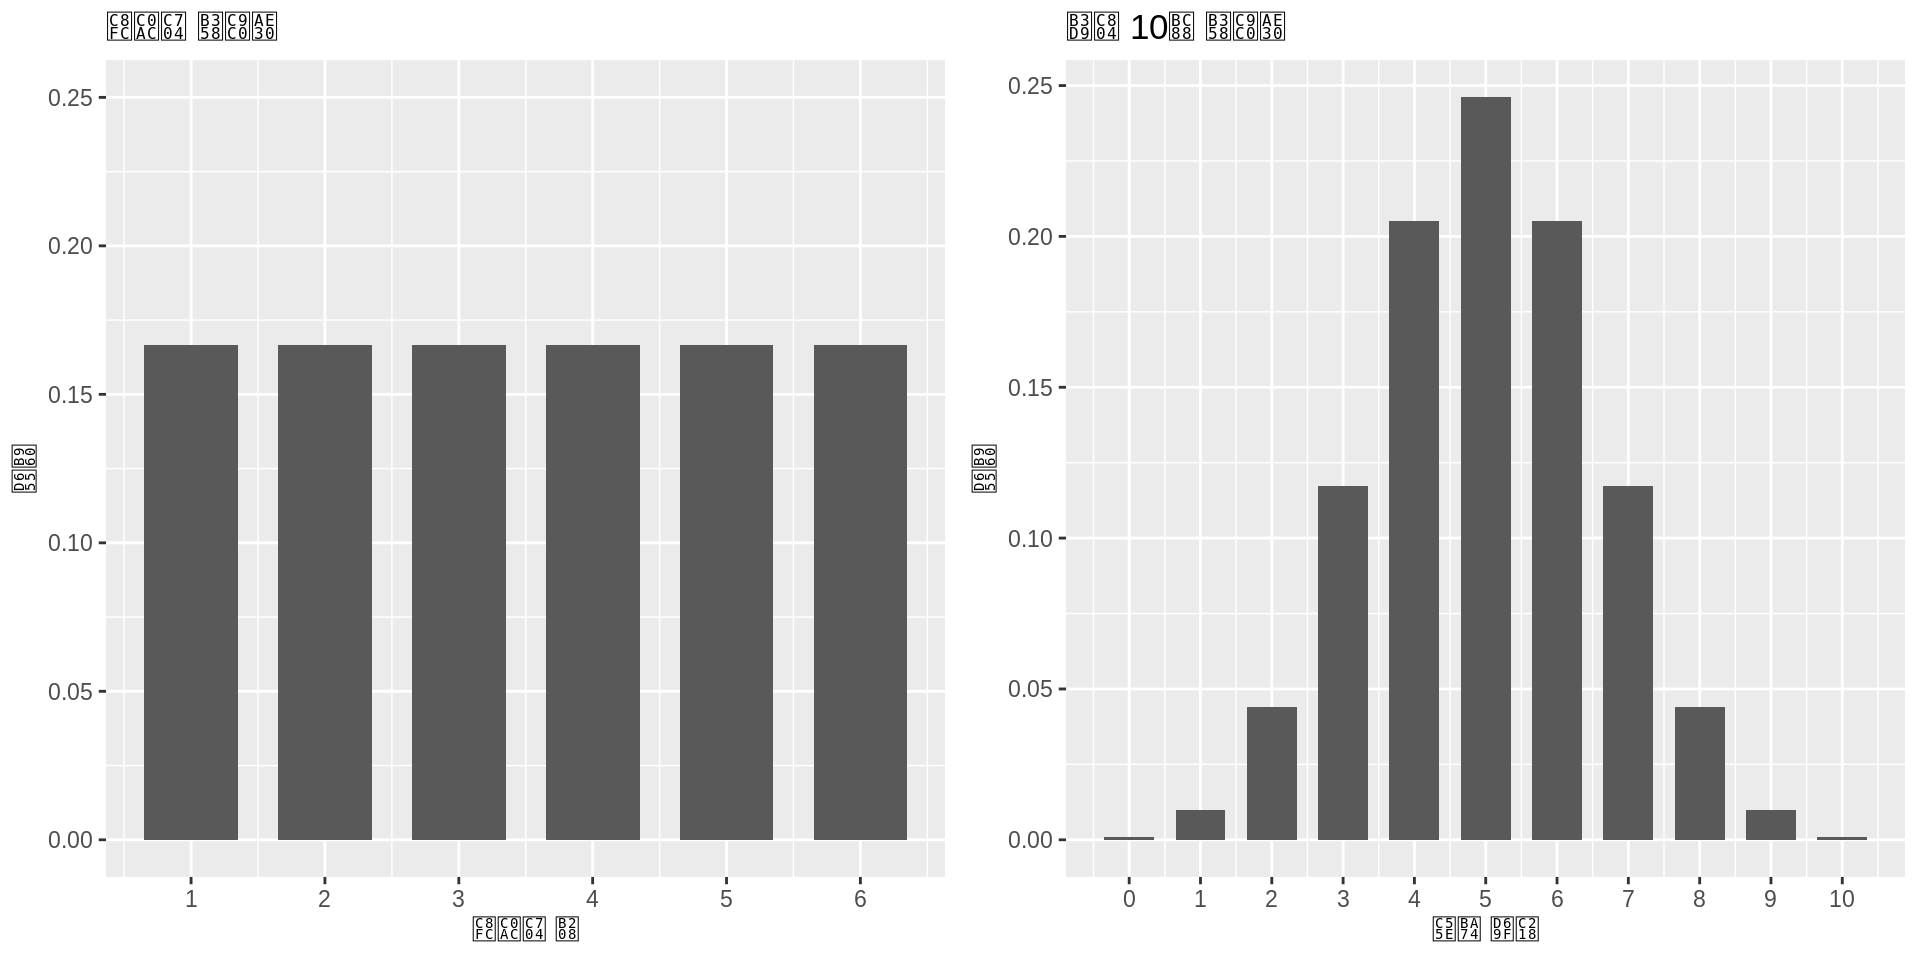
\includegraphics{Basic-stat_files/figure-latex/unnamed-chunk-3-1} 

}

\caption{확률 예시}\label{fig:unnamed-chunk-3}
\end{figure}

\hypertarget{uxc5f0uxc18duxc0acuxac74uxc758-uxd655uxb960}{%
\section{연속사건의 확률}\label{uxc5f0uxc18duxc0acuxac74uxc758-uxd655uxb960}}

\hypertarget{uxd2b9uxc815-uxc0acuxac74uxc758-uxd655uxb960uxc740-uxbaa8uxb450-0}{%
\subsection{특정 사건의 확률은 모두 0}\label{uxd2b9uxc815-uxc0acuxac74uxc758-uxd655uxb960uxc740-uxbaa8uxb450-0}}

이번에는 1에서 6 사이의 숫자 중 랜덤으로 아무 숫자나 뽑는다고 하자. 이 때 정확히 5가 뽑힐 확률은 얼마일까? 1과 6사이에는 무한개의 숫자가 있으니 정확히 5가 뽑힐 확률은 \(\frac{1}{\infty}=0\)이다. 2가 뽑힐 확률, \(\pi\)가 뽑힐 확률도 마찬가지로 0일 뿐만 아니라, 어떤 특정 숫자가 뽑힐 확률은 전부 0이다. 이는 연속된 숫자 사이에서 뽑을 수 있는 숫자의 갯수가 무한하기 때문이다(1과 6사이에는 무한히 많은 숫자가 있다). 따라서 이런 연속사건인 경우 특정 숫자가 나올 확률을 말하는 것은 의미가 없어 다른 방법을 생각해야 하는데, 숫자가 \textbf{특정 구간에 속할 확률}을 말하는 것이 그 대안이다.

\hypertarget{uxd2b9uxc815-uxad6cuxac04uxc5d0-uxc18duxd560-uxd655uxb960-uxd655uxb960uxbc00uxb3c4uxd568uxc218probability-density-function-pdf}{%
\subsection{특정 구간에 속할 확률: 확률밀도함수(Probability Density Function, PDF)}\label{uxd2b9uxc815-uxad6cuxac04uxc5d0-uxc18duxd560-uxd655uxb960-uxd655uxb960uxbc00uxb3c4uxd568uxc218probability-density-function-pdf}}

아까의 1에서 6사이의 숫자를 뽑는 상황을 다시 생각해 보자. 1에서 6사이의 숫자 중 정확히 5가 뽑힐 확률은 0지만 4에서 5사이의 숫자가 뽑힐 확률은 20\%이다. 전체 구간의 길이는 6-1=5이고 4에서 5사이 구간의 길이는 1이기 때문이다. 마찬가지의 논리로 2에서 4사이의 숫자가 뽑힐 확률은 \(\frac{2}{5}=40%\)가 된다. 이처럼 우리는 특정 사건에 대한 확률 대신 특정 구간에 속할 확률을 구함으로서 간접적으로 특정 사건의 확률에 대한 감을 잡을 수 있다. 이것을 설명하는 곡선이 바로 고등학교 때 배운 \textbf{확률밀도함수(Probability Density Function: PDF)}이다. PDF는 특정 구간에 속할 확률을 계산하기 위한 함수이며 함수를 나타내는 \textbf{}이 되게끔 정한 함수이다. 아래 그림을 예를 들어 살펴 보자. 왼쪽의 그림에서 PDF의 값은 1에서 6사이에서는 전부 0.2이고 나머지 구간에서는 전부 0인데, 이는 1에서 6사이의 숫자를 뽑는 상황을 그림으로 나타낸 것이다. 1보다 작거나 6보다 큰 숫자를 뽑을 수는 없으므로 이에 해당하는 확률밀도함수의 함수의 \(y\)값은 전부 0이고, 1\textasciitilde{}6사이에서는 무작위로 숫자를 뽑으므로 \(y\)값은 전부 같다. 전체 확률은 1이므로 그림의 직사각형의 넓이는 1이되고 \(y\)값은 전부 0.2가 되며, 이를 바탕으로 2에서 4사이의 숫자가 뽑힐 확률을 계산하면 \(2\times 0.2=0.4\)로 40\%가 된다. 오른쪽의 그림은 정확한 의미는 잘 몰랐더라도 모양은 많이 봤을 \textbf{정규분포(Normal distribution)}이며, 그 중에서도 가장 흔히 쓰이는 평균 0, 분산 1인 \textbf{표준정규분포(Standard normal distribution)}를 나타내고 있다. 표준정규분포의 PDF는 다들 알고 있는대로(?) \(\frac{1}{\sqrt{2\pi}}e^{-z^2/2}\)로 표현되며 그림에서 보듯이 \(z\)가 -1.96\textasciitilde{}1.96에 안에 있을 확률이 95\%임이 잘 알 려져 있다.

\begin{verbatim}
## Warning in grid.Call(C_textBounds, as.graphicsAnnot(x$label), x$x, x$y, :
## conversion failure on '1~6 중 랜덤으로 숫자 고르기' in 'mbcsToSbcs': dot
## substituted for <ec>
\end{verbatim}

\begin{verbatim}
## Warning in grid.Call(C_textBounds, as.graphicsAnnot(x$label), x$x, x$y, :
## conversion failure on '1~6 중 랜덤으로 숫자 고르기' in 'mbcsToSbcs': dot
## substituted for <a4>
\end{verbatim}

\begin{verbatim}
## Warning in grid.Call(C_textBounds, as.graphicsAnnot(x$label), x$x, x$y, :
## conversion failure on '1~6 중 랜덤으로 숫자 고르기' in 'mbcsToSbcs': dot
## substituted for <91>
\end{verbatim}

\begin{verbatim}
## Warning in grid.Call(C_textBounds, as.graphicsAnnot(x$label), x$x, x$y, :
## conversion failure on '1~6 중 랜덤으로 숫자 고르기' in 'mbcsToSbcs': dot
## substituted for <eb>
\end{verbatim}

\begin{verbatim}
## Warning in grid.Call(C_textBounds, as.graphicsAnnot(x$label), x$x, x$y, :
## conversion failure on '1~6 중 랜덤으로 숫자 고르기' in 'mbcsToSbcs': dot
## substituted for <9e>
\end{verbatim}

\begin{verbatim}
## Warning in grid.Call(C_textBounds, as.graphicsAnnot(x$label), x$x, x$y, :
## conversion failure on '1~6 중 랜덤으로 숫자 고르기' in 'mbcsToSbcs': dot
## substituted for <9c>
\end{verbatim}

\begin{verbatim}
## Warning in grid.Call(C_textBounds, as.graphicsAnnot(x$label), x$x, x$y, :
## conversion failure on '1~6 중 랜덤으로 숫자 고르기' in 'mbcsToSbcs': dot
## substituted for <eb>
\end{verbatim}

\begin{verbatim}
## Warning in grid.Call(C_textBounds, as.graphicsAnnot(x$label), x$x, x$y, :
## conversion failure on '1~6 중 랜덤으로 숫자 고르기' in 'mbcsToSbcs': dot
## substituted for <8d>
\end{verbatim}

\begin{verbatim}
## Warning in grid.Call(C_textBounds, as.graphicsAnnot(x$label), x$x, x$y, :
## conversion failure on '1~6 중 랜덤으로 숫자 고르기' in 'mbcsToSbcs': dot
## substituted for <a4>
\end{verbatim}

\begin{verbatim}
## Warning in grid.Call(C_textBounds, as.graphicsAnnot(x$label), x$x, x$y, :
## conversion failure on '1~6 중 랜덤으로 숫자 고르기' in 'mbcsToSbcs': dot
## substituted for <ec>
\end{verbatim}

\begin{verbatim}
## Warning in grid.Call(C_textBounds, as.graphicsAnnot(x$label), x$x, x$y, :
## conversion failure on '1~6 중 랜덤으로 숫자 고르기' in 'mbcsToSbcs': dot
## substituted for <9c>
\end{verbatim}

\begin{verbatim}
## Warning in grid.Call(C_textBounds, as.graphicsAnnot(x$label), x$x, x$y, :
## conversion failure on '1~6 중 랜덤으로 숫자 고르기' in 'mbcsToSbcs': dot
## substituted for <bc>
\end{verbatim}

\begin{verbatim}
## Warning in grid.Call(C_textBounds, as.graphicsAnnot(x$label), x$x, x$y, :
## conversion failure on '1~6 중 랜덤으로 숫자 고르기' in 'mbcsToSbcs': dot
## substituted for <eb>
\end{verbatim}

\begin{verbatim}
## Warning in grid.Call(C_textBounds, as.graphicsAnnot(x$label), x$x, x$y, :
## conversion failure on '1~6 중 랜덤으로 숫자 고르기' in 'mbcsToSbcs': dot
## substituted for <a1>
\end{verbatim}

\begin{verbatim}
## Warning in grid.Call(C_textBounds, as.graphicsAnnot(x$label), x$x, x$y, :
## conversion failure on '1~6 중 랜덤으로 숫자 고르기' in 'mbcsToSbcs': dot
## substituted for <9c>
\end{verbatim}

\begin{verbatim}
## Warning in grid.Call(C_textBounds, as.graphicsAnnot(x$label), x$x, x$y, :
## conversion failure on '1~6 중 랜덤으로 숫자 고르기' in 'mbcsToSbcs': dot
## substituted for <ec>
\end{verbatim}

\begin{verbatim}
## Warning in grid.Call(C_textBounds, as.graphicsAnnot(x$label), x$x, x$y, :
## conversion failure on '1~6 중 랜덤으로 숫자 고르기' in 'mbcsToSbcs': dot
## substituted for <88>
\end{verbatim}

\begin{verbatim}
## Warning in grid.Call(C_textBounds, as.graphicsAnnot(x$label), x$x, x$y, :
## conversion failure on '1~6 중 랜덤으로 숫자 고르기' in 'mbcsToSbcs': dot
## substituted for <ab>
\end{verbatim}

\begin{verbatim}
## Warning in grid.Call(C_textBounds, as.graphicsAnnot(x$label), x$x, x$y, :
## conversion failure on '1~6 중 랜덤으로 숫자 고르기' in 'mbcsToSbcs': dot
## substituted for <ec>
\end{verbatim}

\begin{verbatim}
## Warning in grid.Call(C_textBounds, as.graphicsAnnot(x$label), x$x, x$y, :
## conversion failure on '1~6 중 랜덤으로 숫자 고르기' in 'mbcsToSbcs': dot
## substituted for <9e>
\end{verbatim}

\begin{verbatim}
## Warning in grid.Call(C_textBounds, as.graphicsAnnot(x$label), x$x, x$y, :
## conversion failure on '1~6 중 랜덤으로 숫자 고르기' in 'mbcsToSbcs': dot
## substituted for <90>
\end{verbatim}

\begin{verbatim}
## Warning in grid.Call(C_textBounds, as.graphicsAnnot(x$label), x$x, x$y, :
## conversion failure on '1~6 중 랜덤으로 숫자 고르기' in 'mbcsToSbcs': dot
## substituted for <ea>
\end{verbatim}

\begin{verbatim}
## Warning in grid.Call(C_textBounds, as.graphicsAnnot(x$label), x$x, x$y, :
## conversion failure on '1~6 중 랜덤으로 숫자 고르기' in 'mbcsToSbcs': dot
## substituted for <b3>
\end{verbatim}

\begin{verbatim}
## Warning in grid.Call(C_textBounds, as.graphicsAnnot(x$label), x$x, x$y, :
## conversion failure on '1~6 중 랜덤으로 숫자 고르기' in 'mbcsToSbcs': dot
## substituted for <a0>
\end{verbatim}

\begin{verbatim}
## Warning in grid.Call(C_textBounds, as.graphicsAnnot(x$label), x$x, x$y, :
## conversion failure on '1~6 중 랜덤으로 숫자 고르기' in 'mbcsToSbcs': dot
## substituted for <eb>
\end{verbatim}

\begin{verbatim}
## Warning in grid.Call(C_textBounds, as.graphicsAnnot(x$label), x$x, x$y, :
## conversion failure on '1~6 중 랜덤으로 숫자 고르기' in 'mbcsToSbcs': dot
## substituted for <a5>
\end{verbatim}

\begin{verbatim}
## Warning in grid.Call(C_textBounds, as.graphicsAnnot(x$label), x$x, x$y, :
## conversion failure on '1~6 중 랜덤으로 숫자 고르기' in 'mbcsToSbcs': dot
## substituted for <b4>
\end{verbatim}

\begin{verbatim}
## Warning in grid.Call(C_textBounds, as.graphicsAnnot(x$label), x$x, x$y, :
## conversion failure on '1~6 중 랜덤으로 숫자 고르기' in 'mbcsToSbcs': dot
## substituted for <ea>
\end{verbatim}

\begin{verbatim}
## Warning in grid.Call(C_textBounds, as.graphicsAnnot(x$label), x$x, x$y, :
## conversion failure on '1~6 중 랜덤으로 숫자 고르기' in 'mbcsToSbcs': dot
## substituted for <b8>
\end{verbatim}

\begin{verbatim}
## Warning in grid.Call(C_textBounds, as.graphicsAnnot(x$label), x$x, x$y, :
## conversion failure on '1~6 중 랜덤으로 숫자 고르기' in 'mbcsToSbcs': dot
## substituted for <b0>
\end{verbatim}

\begin{verbatim}
## Warning in grid.Call(C_textBounds, as.graphicsAnnot(x$label), x$x, x$y, :
## conversion failure on '1~6 중 랜덤으로 숫자 고르기' in 'mbcsToSbcs': dot
## substituted for <ec>
\end{verbatim}

\begin{verbatim}
## Warning in grid.Call(C_textBounds, as.graphicsAnnot(x$label), x$x, x$y, :
## conversion failure on '1~6 중 랜덤으로 숫자 고르기' in 'mbcsToSbcs': dot
## substituted for <a4>
\end{verbatim}

\begin{verbatim}
## Warning in grid.Call(C_textBounds, as.graphicsAnnot(x$label), x$x, x$y, :
## conversion failure on '1~6 중 랜덤으로 숫자 고르기' in 'mbcsToSbcs': dot
## substituted for <91>
\end{verbatim}

\begin{verbatim}
## Warning in grid.Call(C_textBounds, as.graphicsAnnot(x$label), x$x, x$y, :
## conversion failure on '1~6 중 랜덤으로 숫자 고르기' in 'mbcsToSbcs': dot
## substituted for <eb>
\end{verbatim}

\begin{verbatim}
## Warning in grid.Call(C_textBounds, as.graphicsAnnot(x$label), x$x, x$y, :
## conversion failure on '1~6 중 랜덤으로 숫자 고르기' in 'mbcsToSbcs': dot
## substituted for <9e>
\end{verbatim}

\begin{verbatim}
## Warning in grid.Call(C_textBounds, as.graphicsAnnot(x$label), x$x, x$y, :
## conversion failure on '1~6 중 랜덤으로 숫자 고르기' in 'mbcsToSbcs': dot
## substituted for <9c>
\end{verbatim}

\begin{verbatim}
## Warning in grid.Call(C_textBounds, as.graphicsAnnot(x$label), x$x, x$y, :
## conversion failure on '1~6 중 랜덤으로 숫자 고르기' in 'mbcsToSbcs': dot
## substituted for <eb>
\end{verbatim}

\begin{verbatim}
## Warning in grid.Call(C_textBounds, as.graphicsAnnot(x$label), x$x, x$y, :
## conversion failure on '1~6 중 랜덤으로 숫자 고르기' in 'mbcsToSbcs': dot
## substituted for <8d>
\end{verbatim}

\begin{verbatim}
## Warning in grid.Call(C_textBounds, as.graphicsAnnot(x$label), x$x, x$y, :
## conversion failure on '1~6 중 랜덤으로 숫자 고르기' in 'mbcsToSbcs': dot
## substituted for <a4>
\end{verbatim}

\begin{verbatim}
## Warning in grid.Call(C_textBounds, as.graphicsAnnot(x$label), x$x, x$y, :
## conversion failure on '1~6 중 랜덤으로 숫자 고르기' in 'mbcsToSbcs': dot
## substituted for <ec>
\end{verbatim}

\begin{verbatim}
## Warning in grid.Call(C_textBounds, as.graphicsAnnot(x$label), x$x, x$y, :
## conversion failure on '1~6 중 랜덤으로 숫자 고르기' in 'mbcsToSbcs': dot
## substituted for <9c>
\end{verbatim}

\begin{verbatim}
## Warning in grid.Call(C_textBounds, as.graphicsAnnot(x$label), x$x, x$y, :
## conversion failure on '1~6 중 랜덤으로 숫자 고르기' in 'mbcsToSbcs': dot
## substituted for <bc>
\end{verbatim}

\begin{verbatim}
## Warning in grid.Call(C_textBounds, as.graphicsAnnot(x$label), x$x, x$y, :
## conversion failure on '1~6 중 랜덤으로 숫자 고르기' in 'mbcsToSbcs': dot
## substituted for <eb>
\end{verbatim}

\begin{verbatim}
## Warning in grid.Call(C_textBounds, as.graphicsAnnot(x$label), x$x, x$y, :
## conversion failure on '1~6 중 랜덤으로 숫자 고르기' in 'mbcsToSbcs': dot
## substituted for <a1>
\end{verbatim}

\begin{verbatim}
## Warning in grid.Call(C_textBounds, as.graphicsAnnot(x$label), x$x, x$y, :
## conversion failure on '1~6 중 랜덤으로 숫자 고르기' in 'mbcsToSbcs': dot
## substituted for <9c>
\end{verbatim}

\begin{verbatim}
## Warning in grid.Call(C_textBounds, as.graphicsAnnot(x$label), x$x, x$y, :
## conversion failure on '1~6 중 랜덤으로 숫자 고르기' in 'mbcsToSbcs': dot
## substituted for <ec>
\end{verbatim}

\begin{verbatim}
## Warning in grid.Call(C_textBounds, as.graphicsAnnot(x$label), x$x, x$y, :
## conversion failure on '1~6 중 랜덤으로 숫자 고르기' in 'mbcsToSbcs': dot
## substituted for <88>
\end{verbatim}

\begin{verbatim}
## Warning in grid.Call(C_textBounds, as.graphicsAnnot(x$label), x$x, x$y, :
## conversion failure on '1~6 중 랜덤으로 숫자 고르기' in 'mbcsToSbcs': dot
## substituted for <ab>
\end{verbatim}

\begin{verbatim}
## Warning in grid.Call(C_textBounds, as.graphicsAnnot(x$label), x$x, x$y, :
## conversion failure on '1~6 중 랜덤으로 숫자 고르기' in 'mbcsToSbcs': dot
## substituted for <ec>
\end{verbatim}

\begin{verbatim}
## Warning in grid.Call(C_textBounds, as.graphicsAnnot(x$label), x$x, x$y, :
## conversion failure on '1~6 중 랜덤으로 숫자 고르기' in 'mbcsToSbcs': dot
## substituted for <9e>
\end{verbatim}

\begin{verbatim}
## Warning in grid.Call(C_textBounds, as.graphicsAnnot(x$label), x$x, x$y, :
## conversion failure on '1~6 중 랜덤으로 숫자 고르기' in 'mbcsToSbcs': dot
## substituted for <90>
\end{verbatim}

\begin{verbatim}
## Warning in grid.Call(C_textBounds, as.graphicsAnnot(x$label), x$x, x$y, :
## conversion failure on '1~6 중 랜덤으로 숫자 고르기' in 'mbcsToSbcs': dot
## substituted for <ea>
\end{verbatim}

\begin{verbatim}
## Warning in grid.Call(C_textBounds, as.graphicsAnnot(x$label), x$x, x$y, :
## conversion failure on '1~6 중 랜덤으로 숫자 고르기' in 'mbcsToSbcs': dot
## substituted for <b3>
\end{verbatim}

\begin{verbatim}
## Warning in grid.Call(C_textBounds, as.graphicsAnnot(x$label), x$x, x$y, :
## conversion failure on '1~6 중 랜덤으로 숫자 고르기' in 'mbcsToSbcs': dot
## substituted for <a0>
\end{verbatim}

\begin{verbatim}
## Warning in grid.Call(C_textBounds, as.graphicsAnnot(x$label), x$x, x$y, :
## conversion failure on '1~6 중 랜덤으로 숫자 고르기' in 'mbcsToSbcs': dot
## substituted for <eb>
\end{verbatim}

\begin{verbatim}
## Warning in grid.Call(C_textBounds, as.graphicsAnnot(x$label), x$x, x$y, :
## conversion failure on '1~6 중 랜덤으로 숫자 고르기' in 'mbcsToSbcs': dot
## substituted for <a5>
\end{verbatim}

\begin{verbatim}
## Warning in grid.Call(C_textBounds, as.graphicsAnnot(x$label), x$x, x$y, :
## conversion failure on '1~6 중 랜덤으로 숫자 고르기' in 'mbcsToSbcs': dot
## substituted for <b4>
\end{verbatim}

\begin{verbatim}
## Warning in grid.Call(C_textBounds, as.graphicsAnnot(x$label), x$x, x$y, :
## conversion failure on '1~6 중 랜덤으로 숫자 고르기' in 'mbcsToSbcs': dot
## substituted for <ea>
\end{verbatim}

\begin{verbatim}
## Warning in grid.Call(C_textBounds, as.graphicsAnnot(x$label), x$x, x$y, :
## conversion failure on '1~6 중 랜덤으로 숫자 고르기' in 'mbcsToSbcs': dot
## substituted for <b8>
\end{verbatim}

\begin{verbatim}
## Warning in grid.Call(C_textBounds, as.graphicsAnnot(x$label), x$x, x$y, :
## conversion failure on '1~6 중 랜덤으로 숫자 고르기' in 'mbcsToSbcs': dot
## substituted for <b0>
\end{verbatim}

\begin{verbatim}
## Warning in grid.Call(C_textBounds, as.graphicsAnnot(x$label), x$x, x$y, :
## conversion failure on '1~6 중 랜덤으로 숫자 고르기' in 'mbcsToSbcs': dot
## substituted for <ec>
\end{verbatim}

\begin{verbatim}
## Warning in grid.Call(C_textBounds, as.graphicsAnnot(x$label), x$x, x$y, :
## conversion failure on '1~6 중 랜덤으로 숫자 고르기' in 'mbcsToSbcs': dot
## substituted for <a4>
\end{verbatim}

\begin{verbatim}
## Warning in grid.Call(C_textBounds, as.graphicsAnnot(x$label), x$x, x$y, :
## conversion failure on '1~6 중 랜덤으로 숫자 고르기' in 'mbcsToSbcs': dot
## substituted for <91>
\end{verbatim}

\begin{verbatim}
## Warning in grid.Call(C_textBounds, as.graphicsAnnot(x$label), x$x, x$y, :
## conversion failure on '1~6 중 랜덤으로 숫자 고르기' in 'mbcsToSbcs': dot
## substituted for <eb>
\end{verbatim}

\begin{verbatim}
## Warning in grid.Call(C_textBounds, as.graphicsAnnot(x$label), x$x, x$y, :
## conversion failure on '1~6 중 랜덤으로 숫자 고르기' in 'mbcsToSbcs': dot
## substituted for <9e>
\end{verbatim}

\begin{verbatim}
## Warning in grid.Call(C_textBounds, as.graphicsAnnot(x$label), x$x, x$y, :
## conversion failure on '1~6 중 랜덤으로 숫자 고르기' in 'mbcsToSbcs': dot
## substituted for <9c>
\end{verbatim}

\begin{verbatim}
## Warning in grid.Call(C_textBounds, as.graphicsAnnot(x$label), x$x, x$y, :
## conversion failure on '1~6 중 랜덤으로 숫자 고르기' in 'mbcsToSbcs': dot
## substituted for <eb>
\end{verbatim}

\begin{verbatim}
## Warning in grid.Call(C_textBounds, as.graphicsAnnot(x$label), x$x, x$y, :
## conversion failure on '1~6 중 랜덤으로 숫자 고르기' in 'mbcsToSbcs': dot
## substituted for <8d>
\end{verbatim}

\begin{verbatim}
## Warning in grid.Call(C_textBounds, as.graphicsAnnot(x$label), x$x, x$y, :
## conversion failure on '1~6 중 랜덤으로 숫자 고르기' in 'mbcsToSbcs': dot
## substituted for <a4>
\end{verbatim}

\begin{verbatim}
## Warning in grid.Call(C_textBounds, as.graphicsAnnot(x$label), x$x, x$y, :
## conversion failure on '1~6 중 랜덤으로 숫자 고르기' in 'mbcsToSbcs': dot
## substituted for <ec>
\end{verbatim}

\begin{verbatim}
## Warning in grid.Call(C_textBounds, as.graphicsAnnot(x$label), x$x, x$y, :
## conversion failure on '1~6 중 랜덤으로 숫자 고르기' in 'mbcsToSbcs': dot
## substituted for <9c>
\end{verbatim}

\begin{verbatim}
## Warning in grid.Call(C_textBounds, as.graphicsAnnot(x$label), x$x, x$y, :
## conversion failure on '1~6 중 랜덤으로 숫자 고르기' in 'mbcsToSbcs': dot
## substituted for <bc>
\end{verbatim}

\begin{verbatim}
## Warning in grid.Call(C_textBounds, as.graphicsAnnot(x$label), x$x, x$y, :
## conversion failure on '1~6 중 랜덤으로 숫자 고르기' in 'mbcsToSbcs': dot
## substituted for <eb>
\end{verbatim}

\begin{verbatim}
## Warning in grid.Call(C_textBounds, as.graphicsAnnot(x$label), x$x, x$y, :
## conversion failure on '1~6 중 랜덤으로 숫자 고르기' in 'mbcsToSbcs': dot
## substituted for <a1>
\end{verbatim}

\begin{verbatim}
## Warning in grid.Call(C_textBounds, as.graphicsAnnot(x$label), x$x, x$y, :
## conversion failure on '1~6 중 랜덤으로 숫자 고르기' in 'mbcsToSbcs': dot
## substituted for <9c>
\end{verbatim}

\begin{verbatim}
## Warning in grid.Call(C_textBounds, as.graphicsAnnot(x$label), x$x, x$y, :
## conversion failure on '1~6 중 랜덤으로 숫자 고르기' in 'mbcsToSbcs': dot
## substituted for <ec>
\end{verbatim}

\begin{verbatim}
## Warning in grid.Call(C_textBounds, as.graphicsAnnot(x$label), x$x, x$y, :
## conversion failure on '1~6 중 랜덤으로 숫자 고르기' in 'mbcsToSbcs': dot
## substituted for <88>
\end{verbatim}

\begin{verbatim}
## Warning in grid.Call(C_textBounds, as.graphicsAnnot(x$label), x$x, x$y, :
## conversion failure on '1~6 중 랜덤으로 숫자 고르기' in 'mbcsToSbcs': dot
## substituted for <ab>
\end{verbatim}

\begin{verbatim}
## Warning in grid.Call(C_textBounds, as.graphicsAnnot(x$label), x$x, x$y, :
## conversion failure on '1~6 중 랜덤으로 숫자 고르기' in 'mbcsToSbcs': dot
## substituted for <ec>
\end{verbatim}

\begin{verbatim}
## Warning in grid.Call(C_textBounds, as.graphicsAnnot(x$label), x$x, x$y, :
## conversion failure on '1~6 중 랜덤으로 숫자 고르기' in 'mbcsToSbcs': dot
## substituted for <9e>
\end{verbatim}

\begin{verbatim}
## Warning in grid.Call(C_textBounds, as.graphicsAnnot(x$label), x$x, x$y, :
## conversion failure on '1~6 중 랜덤으로 숫자 고르기' in 'mbcsToSbcs': dot
## substituted for <90>
\end{verbatim}

\begin{verbatim}
## Warning in grid.Call(C_textBounds, as.graphicsAnnot(x$label), x$x, x$y, :
## conversion failure on '1~6 중 랜덤으로 숫자 고르기' in 'mbcsToSbcs': dot
## substituted for <ea>
\end{verbatim}

\begin{verbatim}
## Warning in grid.Call(C_textBounds, as.graphicsAnnot(x$label), x$x, x$y, :
## conversion failure on '1~6 중 랜덤으로 숫자 고르기' in 'mbcsToSbcs': dot
## substituted for <b3>
\end{verbatim}

\begin{verbatim}
## Warning in grid.Call(C_textBounds, as.graphicsAnnot(x$label), x$x, x$y, :
## conversion failure on '1~6 중 랜덤으로 숫자 고르기' in 'mbcsToSbcs': dot
## substituted for <a0>
\end{verbatim}

\begin{verbatim}
## Warning in grid.Call(C_textBounds, as.graphicsAnnot(x$label), x$x, x$y, :
## conversion failure on '1~6 중 랜덤으로 숫자 고르기' in 'mbcsToSbcs': dot
## substituted for <eb>
\end{verbatim}

\begin{verbatim}
## Warning in grid.Call(C_textBounds, as.graphicsAnnot(x$label), x$x, x$y, :
## conversion failure on '1~6 중 랜덤으로 숫자 고르기' in 'mbcsToSbcs': dot
## substituted for <a5>
\end{verbatim}

\begin{verbatim}
## Warning in grid.Call(C_textBounds, as.graphicsAnnot(x$label), x$x, x$y, :
## conversion failure on '1~6 중 랜덤으로 숫자 고르기' in 'mbcsToSbcs': dot
## substituted for <b4>
\end{verbatim}

\begin{verbatim}
## Warning in grid.Call(C_textBounds, as.graphicsAnnot(x$label), x$x, x$y, :
## conversion failure on '1~6 중 랜덤으로 숫자 고르기' in 'mbcsToSbcs': dot
## substituted for <ea>
\end{verbatim}

\begin{verbatim}
## Warning in grid.Call(C_textBounds, as.graphicsAnnot(x$label), x$x, x$y, :
## conversion failure on '1~6 중 랜덤으로 숫자 고르기' in 'mbcsToSbcs': dot
## substituted for <b8>
\end{verbatim}

\begin{verbatim}
## Warning in grid.Call(C_textBounds, as.graphicsAnnot(x$label), x$x, x$y, :
## conversion failure on '1~6 중 랜덤으로 숫자 고르기' in 'mbcsToSbcs': dot
## substituted for <b0>
\end{verbatim}

\begin{verbatim}
## Warning in grid.Call(C_textBounds, as.graphicsAnnot(x$label), x$x, x$y, :
## conversion failure on '1~6 중 랜덤으로 숫자 고르기' in 'mbcsToSbcs': dot
## substituted for <ec>
\end{verbatim}

\begin{verbatim}
## Warning in grid.Call(C_textBounds, as.graphicsAnnot(x$label), x$x, x$y, :
## conversion failure on '1~6 중 랜덤으로 숫자 고르기' in 'mbcsToSbcs': dot
## substituted for <a4>
\end{verbatim}

\begin{verbatim}
## Warning in grid.Call(C_textBounds, as.graphicsAnnot(x$label), x$x, x$y, :
## conversion failure on '1~6 중 랜덤으로 숫자 고르기' in 'mbcsToSbcs': dot
## substituted for <91>
\end{verbatim}

\begin{verbatim}
## Warning in grid.Call(C_textBounds, as.graphicsAnnot(x$label), x$x, x$y, :
## conversion failure on '1~6 중 랜덤으로 숫자 고르기' in 'mbcsToSbcs': dot
## substituted for <eb>
\end{verbatim}

\begin{verbatim}
## Warning in grid.Call(C_textBounds, as.graphicsAnnot(x$label), x$x, x$y, :
## conversion failure on '1~6 중 랜덤으로 숫자 고르기' in 'mbcsToSbcs': dot
## substituted for <9e>
\end{verbatim}

\begin{verbatim}
## Warning in grid.Call(C_textBounds, as.graphicsAnnot(x$label), x$x, x$y, :
## conversion failure on '1~6 중 랜덤으로 숫자 고르기' in 'mbcsToSbcs': dot
## substituted for <9c>
\end{verbatim}

\begin{verbatim}
## Warning in grid.Call(C_textBounds, as.graphicsAnnot(x$label), x$x, x$y, :
## conversion failure on '1~6 중 랜덤으로 숫자 고르기' in 'mbcsToSbcs': dot
## substituted for <eb>
\end{verbatim}

\begin{verbatim}
## Warning in grid.Call(C_textBounds, as.graphicsAnnot(x$label), x$x, x$y, :
## conversion failure on '1~6 중 랜덤으로 숫자 고르기' in 'mbcsToSbcs': dot
## substituted for <8d>
\end{verbatim}

\begin{verbatim}
## Warning in grid.Call(C_textBounds, as.graphicsAnnot(x$label), x$x, x$y, :
## conversion failure on '1~6 중 랜덤으로 숫자 고르기' in 'mbcsToSbcs': dot
## substituted for <a4>
\end{verbatim}

\begin{verbatim}
## Warning in grid.Call(C_textBounds, as.graphicsAnnot(x$label), x$x, x$y, :
## conversion failure on '1~6 중 랜덤으로 숫자 고르기' in 'mbcsToSbcs': dot
## substituted for <ec>
\end{verbatim}

\begin{verbatim}
## Warning in grid.Call(C_textBounds, as.graphicsAnnot(x$label), x$x, x$y, :
## conversion failure on '1~6 중 랜덤으로 숫자 고르기' in 'mbcsToSbcs': dot
## substituted for <9c>
\end{verbatim}

\begin{verbatim}
## Warning in grid.Call(C_textBounds, as.graphicsAnnot(x$label), x$x, x$y, :
## conversion failure on '1~6 중 랜덤으로 숫자 고르기' in 'mbcsToSbcs': dot
## substituted for <bc>
\end{verbatim}

\begin{verbatim}
## Warning in grid.Call(C_textBounds, as.graphicsAnnot(x$label), x$x, x$y, :
## conversion failure on '1~6 중 랜덤으로 숫자 고르기' in 'mbcsToSbcs': dot
## substituted for <eb>
\end{verbatim}

\begin{verbatim}
## Warning in grid.Call(C_textBounds, as.graphicsAnnot(x$label), x$x, x$y, :
## conversion failure on '1~6 중 랜덤으로 숫자 고르기' in 'mbcsToSbcs': dot
## substituted for <a1>
\end{verbatim}

\begin{verbatim}
## Warning in grid.Call(C_textBounds, as.graphicsAnnot(x$label), x$x, x$y, :
## conversion failure on '1~6 중 랜덤으로 숫자 고르기' in 'mbcsToSbcs': dot
## substituted for <9c>
\end{verbatim}

\begin{verbatim}
## Warning in grid.Call(C_textBounds, as.graphicsAnnot(x$label), x$x, x$y, :
## conversion failure on '1~6 중 랜덤으로 숫자 고르기' in 'mbcsToSbcs': dot
## substituted for <ec>
\end{verbatim}

\begin{verbatim}
## Warning in grid.Call(C_textBounds, as.graphicsAnnot(x$label), x$x, x$y, :
## conversion failure on '1~6 중 랜덤으로 숫자 고르기' in 'mbcsToSbcs': dot
## substituted for <88>
\end{verbatim}

\begin{verbatim}
## Warning in grid.Call(C_textBounds, as.graphicsAnnot(x$label), x$x, x$y, :
## conversion failure on '1~6 중 랜덤으로 숫자 고르기' in 'mbcsToSbcs': dot
## substituted for <ab>
\end{verbatim}

\begin{verbatim}
## Warning in grid.Call(C_textBounds, as.graphicsAnnot(x$label), x$x, x$y, :
## conversion failure on '1~6 중 랜덤으로 숫자 고르기' in 'mbcsToSbcs': dot
## substituted for <ec>
\end{verbatim}

\begin{verbatim}
## Warning in grid.Call(C_textBounds, as.graphicsAnnot(x$label), x$x, x$y, :
## conversion failure on '1~6 중 랜덤으로 숫자 고르기' in 'mbcsToSbcs': dot
## substituted for <9e>
\end{verbatim}

\begin{verbatim}
## Warning in grid.Call(C_textBounds, as.graphicsAnnot(x$label), x$x, x$y, :
## conversion failure on '1~6 중 랜덤으로 숫자 고르기' in 'mbcsToSbcs': dot
## substituted for <90>
\end{verbatim}

\begin{verbatim}
## Warning in grid.Call(C_textBounds, as.graphicsAnnot(x$label), x$x, x$y, :
## conversion failure on '1~6 중 랜덤으로 숫자 고르기' in 'mbcsToSbcs': dot
## substituted for <ea>
\end{verbatim}

\begin{verbatim}
## Warning in grid.Call(C_textBounds, as.graphicsAnnot(x$label), x$x, x$y, :
## conversion failure on '1~6 중 랜덤으로 숫자 고르기' in 'mbcsToSbcs': dot
## substituted for <b3>
\end{verbatim}

\begin{verbatim}
## Warning in grid.Call(C_textBounds, as.graphicsAnnot(x$label), x$x, x$y, :
## conversion failure on '1~6 중 랜덤으로 숫자 고르기' in 'mbcsToSbcs': dot
## substituted for <a0>
\end{verbatim}

\begin{verbatim}
## Warning in grid.Call(C_textBounds, as.graphicsAnnot(x$label), x$x, x$y, :
## conversion failure on '1~6 중 랜덤으로 숫자 고르기' in 'mbcsToSbcs': dot
## substituted for <eb>
\end{verbatim}

\begin{verbatim}
## Warning in grid.Call(C_textBounds, as.graphicsAnnot(x$label), x$x, x$y, :
## conversion failure on '1~6 중 랜덤으로 숫자 고르기' in 'mbcsToSbcs': dot
## substituted for <a5>
\end{verbatim}

\begin{verbatim}
## Warning in grid.Call(C_textBounds, as.graphicsAnnot(x$label), x$x, x$y, :
## conversion failure on '1~6 중 랜덤으로 숫자 고르기' in 'mbcsToSbcs': dot
## substituted for <b4>
\end{verbatim}

\begin{verbatim}
## Warning in grid.Call(C_textBounds, as.graphicsAnnot(x$label), x$x, x$y, :
## conversion failure on '1~6 중 랜덤으로 숫자 고르기' in 'mbcsToSbcs': dot
## substituted for <ea>
\end{verbatim}

\begin{verbatim}
## Warning in grid.Call(C_textBounds, as.graphicsAnnot(x$label), x$x, x$y, :
## conversion failure on '1~6 중 랜덤으로 숫자 고르기' in 'mbcsToSbcs': dot
## substituted for <b8>
\end{verbatim}

\begin{verbatim}
## Warning in grid.Call(C_textBounds, as.graphicsAnnot(x$label), x$x, x$y, :
## conversion failure on '1~6 중 랜덤으로 숫자 고르기' in 'mbcsToSbcs': dot
## substituted for <b0>
\end{verbatim}

\begin{verbatim}
## Warning in grid.Call(C_textBounds, as.graphicsAnnot(x$label), x$x, x$y, :
## conversion failure on '1~6 중 랜덤으로 숫자 고르기' in 'mbcsToSbcs': dot
## substituted for <ec>
\end{verbatim}

\begin{verbatim}
## Warning in grid.Call(C_textBounds, as.graphicsAnnot(x$label), x$x, x$y, :
## conversion failure on '1~6 중 랜덤으로 숫자 고르기' in 'mbcsToSbcs': dot
## substituted for <a4>
\end{verbatim}

\begin{verbatim}
## Warning in grid.Call(C_textBounds, as.graphicsAnnot(x$label), x$x, x$y, :
## conversion failure on '1~6 중 랜덤으로 숫자 고르기' in 'mbcsToSbcs': dot
## substituted for <91>
\end{verbatim}

\begin{verbatim}
## Warning in grid.Call(C_textBounds, as.graphicsAnnot(x$label), x$x, x$y, :
## conversion failure on '1~6 중 랜덤으로 숫자 고르기' in 'mbcsToSbcs': dot
## substituted for <eb>
\end{verbatim}

\begin{verbatim}
## Warning in grid.Call(C_textBounds, as.graphicsAnnot(x$label), x$x, x$y, :
## conversion failure on '1~6 중 랜덤으로 숫자 고르기' in 'mbcsToSbcs': dot
## substituted for <9e>
\end{verbatim}

\begin{verbatim}
## Warning in grid.Call(C_textBounds, as.graphicsAnnot(x$label), x$x, x$y, :
## conversion failure on '1~6 중 랜덤으로 숫자 고르기' in 'mbcsToSbcs': dot
## substituted for <9c>
\end{verbatim}

\begin{verbatim}
## Warning in grid.Call(C_textBounds, as.graphicsAnnot(x$label), x$x, x$y, :
## conversion failure on '1~6 중 랜덤으로 숫자 고르기' in 'mbcsToSbcs': dot
## substituted for <eb>
\end{verbatim}

\begin{verbatim}
## Warning in grid.Call(C_textBounds, as.graphicsAnnot(x$label), x$x, x$y, :
## conversion failure on '1~6 중 랜덤으로 숫자 고르기' in 'mbcsToSbcs': dot
## substituted for <8d>
\end{verbatim}

\begin{verbatim}
## Warning in grid.Call(C_textBounds, as.graphicsAnnot(x$label), x$x, x$y, :
## conversion failure on '1~6 중 랜덤으로 숫자 고르기' in 'mbcsToSbcs': dot
## substituted for <a4>
\end{verbatim}

\begin{verbatim}
## Warning in grid.Call(C_textBounds, as.graphicsAnnot(x$label), x$x, x$y, :
## conversion failure on '1~6 중 랜덤으로 숫자 고르기' in 'mbcsToSbcs': dot
## substituted for <ec>
\end{verbatim}

\begin{verbatim}
## Warning in grid.Call(C_textBounds, as.graphicsAnnot(x$label), x$x, x$y, :
## conversion failure on '1~6 중 랜덤으로 숫자 고르기' in 'mbcsToSbcs': dot
## substituted for <9c>
\end{verbatim}

\begin{verbatim}
## Warning in grid.Call(C_textBounds, as.graphicsAnnot(x$label), x$x, x$y, :
## conversion failure on '1~6 중 랜덤으로 숫자 고르기' in 'mbcsToSbcs': dot
## substituted for <bc>
\end{verbatim}

\begin{verbatim}
## Warning in grid.Call(C_textBounds, as.graphicsAnnot(x$label), x$x, x$y, :
## conversion failure on '1~6 중 랜덤으로 숫자 고르기' in 'mbcsToSbcs': dot
## substituted for <eb>
\end{verbatim}

\begin{verbatim}
## Warning in grid.Call(C_textBounds, as.graphicsAnnot(x$label), x$x, x$y, :
## conversion failure on '1~6 중 랜덤으로 숫자 고르기' in 'mbcsToSbcs': dot
## substituted for <a1>
\end{verbatim}

\begin{verbatim}
## Warning in grid.Call(C_textBounds, as.graphicsAnnot(x$label), x$x, x$y, :
## conversion failure on '1~6 중 랜덤으로 숫자 고르기' in 'mbcsToSbcs': dot
## substituted for <9c>
\end{verbatim}

\begin{verbatim}
## Warning in grid.Call(C_textBounds, as.graphicsAnnot(x$label), x$x, x$y, :
## conversion failure on '1~6 중 랜덤으로 숫자 고르기' in 'mbcsToSbcs': dot
## substituted for <ec>
\end{verbatim}

\begin{verbatim}
## Warning in grid.Call(C_textBounds, as.graphicsAnnot(x$label), x$x, x$y, :
## conversion failure on '1~6 중 랜덤으로 숫자 고르기' in 'mbcsToSbcs': dot
## substituted for <88>
\end{verbatim}

\begin{verbatim}
## Warning in grid.Call(C_textBounds, as.graphicsAnnot(x$label), x$x, x$y, :
## conversion failure on '1~6 중 랜덤으로 숫자 고르기' in 'mbcsToSbcs': dot
## substituted for <ab>
\end{verbatim}

\begin{verbatim}
## Warning in grid.Call(C_textBounds, as.graphicsAnnot(x$label), x$x, x$y, :
## conversion failure on '1~6 중 랜덤으로 숫자 고르기' in 'mbcsToSbcs': dot
## substituted for <ec>
\end{verbatim}

\begin{verbatim}
## Warning in grid.Call(C_textBounds, as.graphicsAnnot(x$label), x$x, x$y, :
## conversion failure on '1~6 중 랜덤으로 숫자 고르기' in 'mbcsToSbcs': dot
## substituted for <9e>
\end{verbatim}

\begin{verbatim}
## Warning in grid.Call(C_textBounds, as.graphicsAnnot(x$label), x$x, x$y, :
## conversion failure on '1~6 중 랜덤으로 숫자 고르기' in 'mbcsToSbcs': dot
## substituted for <90>
\end{verbatim}

\begin{verbatim}
## Warning in grid.Call(C_textBounds, as.graphicsAnnot(x$label), x$x, x$y, :
## conversion failure on '1~6 중 랜덤으로 숫자 고르기' in 'mbcsToSbcs': dot
## substituted for <ea>
\end{verbatim}

\begin{verbatim}
## Warning in grid.Call(C_textBounds, as.graphicsAnnot(x$label), x$x, x$y, :
## conversion failure on '1~6 중 랜덤으로 숫자 고르기' in 'mbcsToSbcs': dot
## substituted for <b3>
\end{verbatim}

\begin{verbatim}
## Warning in grid.Call(C_textBounds, as.graphicsAnnot(x$label), x$x, x$y, :
## conversion failure on '1~6 중 랜덤으로 숫자 고르기' in 'mbcsToSbcs': dot
## substituted for <a0>
\end{verbatim}

\begin{verbatim}
## Warning in grid.Call(C_textBounds, as.graphicsAnnot(x$label), x$x, x$y, :
## conversion failure on '1~6 중 랜덤으로 숫자 고르기' in 'mbcsToSbcs': dot
## substituted for <eb>
\end{verbatim}

\begin{verbatim}
## Warning in grid.Call(C_textBounds, as.graphicsAnnot(x$label), x$x, x$y, :
## conversion failure on '1~6 중 랜덤으로 숫자 고르기' in 'mbcsToSbcs': dot
## substituted for <a5>
\end{verbatim}

\begin{verbatim}
## Warning in grid.Call(C_textBounds, as.graphicsAnnot(x$label), x$x, x$y, :
## conversion failure on '1~6 중 랜덤으로 숫자 고르기' in 'mbcsToSbcs': dot
## substituted for <b4>
\end{verbatim}

\begin{verbatim}
## Warning in grid.Call(C_textBounds, as.graphicsAnnot(x$label), x$x, x$y, :
## conversion failure on '1~6 중 랜덤으로 숫자 고르기' in 'mbcsToSbcs': dot
## substituted for <ea>
\end{verbatim}

\begin{verbatim}
## Warning in grid.Call(C_textBounds, as.graphicsAnnot(x$label), x$x, x$y, :
## conversion failure on '1~6 중 랜덤으로 숫자 고르기' in 'mbcsToSbcs': dot
## substituted for <b8>
\end{verbatim}

\begin{verbatim}
## Warning in grid.Call(C_textBounds, as.graphicsAnnot(x$label), x$x, x$y, :
## conversion failure on '1~6 중 랜덤으로 숫자 고르기' in 'mbcsToSbcs': dot
## substituted for <b0>
\end{verbatim}

\begin{verbatim}
## Warning in grid.Call(C_textBounds, as.graphicsAnnot(x$label), x$x, x$y, :
## conversion failure on '1~6 중 랜덤으로 숫자 고르기' in 'mbcsToSbcs': dot
## substituted for <ec>
\end{verbatim}

\begin{verbatim}
## Warning in grid.Call(C_textBounds, as.graphicsAnnot(x$label), x$x, x$y, :
## conversion failure on '1~6 중 랜덤으로 숫자 고르기' in 'mbcsToSbcs': dot
## substituted for <a4>
\end{verbatim}

\begin{verbatim}
## Warning in grid.Call(C_textBounds, as.graphicsAnnot(x$label), x$x, x$y, :
## conversion failure on '1~6 중 랜덤으로 숫자 고르기' in 'mbcsToSbcs': dot
## substituted for <91>
\end{verbatim}

\begin{verbatim}
## Warning in grid.Call(C_textBounds, as.graphicsAnnot(x$label), x$x, x$y, :
## conversion failure on '1~6 중 랜덤으로 숫자 고르기' in 'mbcsToSbcs': dot
## substituted for <eb>
\end{verbatim}

\begin{verbatim}
## Warning in grid.Call(C_textBounds, as.graphicsAnnot(x$label), x$x, x$y, :
## conversion failure on '1~6 중 랜덤으로 숫자 고르기' in 'mbcsToSbcs': dot
## substituted for <9e>
\end{verbatim}

\begin{verbatim}
## Warning in grid.Call(C_textBounds, as.graphicsAnnot(x$label), x$x, x$y, :
## conversion failure on '1~6 중 랜덤으로 숫자 고르기' in 'mbcsToSbcs': dot
## substituted for <9c>
\end{verbatim}

\begin{verbatim}
## Warning in grid.Call(C_textBounds, as.graphicsAnnot(x$label), x$x, x$y, :
## conversion failure on '1~6 중 랜덤으로 숫자 고르기' in 'mbcsToSbcs': dot
## substituted for <eb>
\end{verbatim}

\begin{verbatim}
## Warning in grid.Call(C_textBounds, as.graphicsAnnot(x$label), x$x, x$y, :
## conversion failure on '1~6 중 랜덤으로 숫자 고르기' in 'mbcsToSbcs': dot
## substituted for <8d>
\end{verbatim}

\begin{verbatim}
## Warning in grid.Call(C_textBounds, as.graphicsAnnot(x$label), x$x, x$y, :
## conversion failure on '1~6 중 랜덤으로 숫자 고르기' in 'mbcsToSbcs': dot
## substituted for <a4>
\end{verbatim}

\begin{verbatim}
## Warning in grid.Call(C_textBounds, as.graphicsAnnot(x$label), x$x, x$y, :
## conversion failure on '1~6 중 랜덤으로 숫자 고르기' in 'mbcsToSbcs': dot
## substituted for <ec>
\end{verbatim}

\begin{verbatim}
## Warning in grid.Call(C_textBounds, as.graphicsAnnot(x$label), x$x, x$y, :
## conversion failure on '1~6 중 랜덤으로 숫자 고르기' in 'mbcsToSbcs': dot
## substituted for <9c>
\end{verbatim}

\begin{verbatim}
## Warning in grid.Call(C_textBounds, as.graphicsAnnot(x$label), x$x, x$y, :
## conversion failure on '1~6 중 랜덤으로 숫자 고르기' in 'mbcsToSbcs': dot
## substituted for <bc>
\end{verbatim}

\begin{verbatim}
## Warning in grid.Call(C_textBounds, as.graphicsAnnot(x$label), x$x, x$y, :
## conversion failure on '1~6 중 랜덤으로 숫자 고르기' in 'mbcsToSbcs': dot
## substituted for <eb>
\end{verbatim}

\begin{verbatim}
## Warning in grid.Call(C_textBounds, as.graphicsAnnot(x$label), x$x, x$y, :
## conversion failure on '1~6 중 랜덤으로 숫자 고르기' in 'mbcsToSbcs': dot
## substituted for <a1>
\end{verbatim}

\begin{verbatim}
## Warning in grid.Call(C_textBounds, as.graphicsAnnot(x$label), x$x, x$y, :
## conversion failure on '1~6 중 랜덤으로 숫자 고르기' in 'mbcsToSbcs': dot
## substituted for <9c>
\end{verbatim}

\begin{verbatim}
## Warning in grid.Call(C_textBounds, as.graphicsAnnot(x$label), x$x, x$y, :
## conversion failure on '1~6 중 랜덤으로 숫자 고르기' in 'mbcsToSbcs': dot
## substituted for <ec>
\end{verbatim}

\begin{verbatim}
## Warning in grid.Call(C_textBounds, as.graphicsAnnot(x$label), x$x, x$y, :
## conversion failure on '1~6 중 랜덤으로 숫자 고르기' in 'mbcsToSbcs': dot
## substituted for <88>
\end{verbatim}

\begin{verbatim}
## Warning in grid.Call(C_textBounds, as.graphicsAnnot(x$label), x$x, x$y, :
## conversion failure on '1~6 중 랜덤으로 숫자 고르기' in 'mbcsToSbcs': dot
## substituted for <ab>
\end{verbatim}

\begin{verbatim}
## Warning in grid.Call(C_textBounds, as.graphicsAnnot(x$label), x$x, x$y, :
## conversion failure on '1~6 중 랜덤으로 숫자 고르기' in 'mbcsToSbcs': dot
## substituted for <ec>
\end{verbatim}

\begin{verbatim}
## Warning in grid.Call(C_textBounds, as.graphicsAnnot(x$label), x$x, x$y, :
## conversion failure on '1~6 중 랜덤으로 숫자 고르기' in 'mbcsToSbcs': dot
## substituted for <9e>
\end{verbatim}

\begin{verbatim}
## Warning in grid.Call(C_textBounds, as.graphicsAnnot(x$label), x$x, x$y, :
## conversion failure on '1~6 중 랜덤으로 숫자 고르기' in 'mbcsToSbcs': dot
## substituted for <90>
\end{verbatim}

\begin{verbatim}
## Warning in grid.Call(C_textBounds, as.graphicsAnnot(x$label), x$x, x$y, :
## conversion failure on '1~6 중 랜덤으로 숫자 고르기' in 'mbcsToSbcs': dot
## substituted for <ea>
\end{verbatim}

\begin{verbatim}
## Warning in grid.Call(C_textBounds, as.graphicsAnnot(x$label), x$x, x$y, :
## conversion failure on '1~6 중 랜덤으로 숫자 고르기' in 'mbcsToSbcs': dot
## substituted for <b3>
\end{verbatim}

\begin{verbatim}
## Warning in grid.Call(C_textBounds, as.graphicsAnnot(x$label), x$x, x$y, :
## conversion failure on '1~6 중 랜덤으로 숫자 고르기' in 'mbcsToSbcs': dot
## substituted for <a0>
\end{verbatim}

\begin{verbatim}
## Warning in grid.Call(C_textBounds, as.graphicsAnnot(x$label), x$x, x$y, :
## conversion failure on '1~6 중 랜덤으로 숫자 고르기' in 'mbcsToSbcs': dot
## substituted for <eb>
\end{verbatim}

\begin{verbatim}
## Warning in grid.Call(C_textBounds, as.graphicsAnnot(x$label), x$x, x$y, :
## conversion failure on '1~6 중 랜덤으로 숫자 고르기' in 'mbcsToSbcs': dot
## substituted for <a5>
\end{verbatim}

\begin{verbatim}
## Warning in grid.Call(C_textBounds, as.graphicsAnnot(x$label), x$x, x$y, :
## conversion failure on '1~6 중 랜덤으로 숫자 고르기' in 'mbcsToSbcs': dot
## substituted for <b4>
\end{verbatim}

\begin{verbatim}
## Warning in grid.Call(C_textBounds, as.graphicsAnnot(x$label), x$x, x$y, :
## conversion failure on '1~6 중 랜덤으로 숫자 고르기' in 'mbcsToSbcs': dot
## substituted for <ea>
\end{verbatim}

\begin{verbatim}
## Warning in grid.Call(C_textBounds, as.graphicsAnnot(x$label), x$x, x$y, :
## conversion failure on '1~6 중 랜덤으로 숫자 고르기' in 'mbcsToSbcs': dot
## substituted for <b8>
\end{verbatim}

\begin{verbatim}
## Warning in grid.Call(C_textBounds, as.graphicsAnnot(x$label), x$x, x$y, :
## conversion failure on '1~6 중 랜덤으로 숫자 고르기' in 'mbcsToSbcs': dot
## substituted for <b0>
\end{verbatim}

\begin{verbatim}
## Warning in grid.Call(C_textBounds, as.graphicsAnnot(x$label), x$x, x$y, :
## conversion failure on '1~6 중 랜덤으로 숫자 고르기' in 'mbcsToSbcs': dot
## substituted for <ec>
\end{verbatim}

\begin{verbatim}
## Warning in grid.Call(C_textBounds, as.graphicsAnnot(x$label), x$x, x$y, :
## conversion failure on '1~6 중 랜덤으로 숫자 고르기' in 'mbcsToSbcs': dot
## substituted for <a4>
\end{verbatim}

\begin{verbatim}
## Warning in grid.Call(C_textBounds, as.graphicsAnnot(x$label), x$x, x$y, :
## conversion failure on '1~6 중 랜덤으로 숫자 고르기' in 'mbcsToSbcs': dot
## substituted for <91>
\end{verbatim}

\begin{verbatim}
## Warning in grid.Call(C_textBounds, as.graphicsAnnot(x$label), x$x, x$y, :
## conversion failure on '1~6 중 랜덤으로 숫자 고르기' in 'mbcsToSbcs': dot
## substituted for <eb>
\end{verbatim}

\begin{verbatim}
## Warning in grid.Call(C_textBounds, as.graphicsAnnot(x$label), x$x, x$y, :
## conversion failure on '1~6 중 랜덤으로 숫자 고르기' in 'mbcsToSbcs': dot
## substituted for <9e>
\end{verbatim}

\begin{verbatim}
## Warning in grid.Call(C_textBounds, as.graphicsAnnot(x$label), x$x, x$y, :
## conversion failure on '1~6 중 랜덤으로 숫자 고르기' in 'mbcsToSbcs': dot
## substituted for <9c>
\end{verbatim}

\begin{verbatim}
## Warning in grid.Call(C_textBounds, as.graphicsAnnot(x$label), x$x, x$y, :
## conversion failure on '1~6 중 랜덤으로 숫자 고르기' in 'mbcsToSbcs': dot
## substituted for <eb>
\end{verbatim}

\begin{verbatim}
## Warning in grid.Call(C_textBounds, as.graphicsAnnot(x$label), x$x, x$y, :
## conversion failure on '1~6 중 랜덤으로 숫자 고르기' in 'mbcsToSbcs': dot
## substituted for <8d>
\end{verbatim}

\begin{verbatim}
## Warning in grid.Call(C_textBounds, as.graphicsAnnot(x$label), x$x, x$y, :
## conversion failure on '1~6 중 랜덤으로 숫자 고르기' in 'mbcsToSbcs': dot
## substituted for <a4>
\end{verbatim}

\begin{verbatim}
## Warning in grid.Call(C_textBounds, as.graphicsAnnot(x$label), x$x, x$y, :
## conversion failure on '1~6 중 랜덤으로 숫자 고르기' in 'mbcsToSbcs': dot
## substituted for <ec>
\end{verbatim}

\begin{verbatim}
## Warning in grid.Call(C_textBounds, as.graphicsAnnot(x$label), x$x, x$y, :
## conversion failure on '1~6 중 랜덤으로 숫자 고르기' in 'mbcsToSbcs': dot
## substituted for <9c>
\end{verbatim}

\begin{verbatim}
## Warning in grid.Call(C_textBounds, as.graphicsAnnot(x$label), x$x, x$y, :
## conversion failure on '1~6 중 랜덤으로 숫자 고르기' in 'mbcsToSbcs': dot
## substituted for <bc>
\end{verbatim}

\begin{verbatim}
## Warning in grid.Call(C_textBounds, as.graphicsAnnot(x$label), x$x, x$y, :
## conversion failure on '1~6 중 랜덤으로 숫자 고르기' in 'mbcsToSbcs': dot
## substituted for <eb>
\end{verbatim}

\begin{verbatim}
## Warning in grid.Call(C_textBounds, as.graphicsAnnot(x$label), x$x, x$y, :
## conversion failure on '1~6 중 랜덤으로 숫자 고르기' in 'mbcsToSbcs': dot
## substituted for <a1>
\end{verbatim}

\begin{verbatim}
## Warning in grid.Call(C_textBounds, as.graphicsAnnot(x$label), x$x, x$y, :
## conversion failure on '1~6 중 랜덤으로 숫자 고르기' in 'mbcsToSbcs': dot
## substituted for <9c>
\end{verbatim}

\begin{verbatim}
## Warning in grid.Call(C_textBounds, as.graphicsAnnot(x$label), x$x, x$y, :
## conversion failure on '1~6 중 랜덤으로 숫자 고르기' in 'mbcsToSbcs': dot
## substituted for <ec>
\end{verbatim}

\begin{verbatim}
## Warning in grid.Call(C_textBounds, as.graphicsAnnot(x$label), x$x, x$y, :
## conversion failure on '1~6 중 랜덤으로 숫자 고르기' in 'mbcsToSbcs': dot
## substituted for <88>
\end{verbatim}

\begin{verbatim}
## Warning in grid.Call(C_textBounds, as.graphicsAnnot(x$label), x$x, x$y, :
## conversion failure on '1~6 중 랜덤으로 숫자 고르기' in 'mbcsToSbcs': dot
## substituted for <ab>
\end{verbatim}

\begin{verbatim}
## Warning in grid.Call(C_textBounds, as.graphicsAnnot(x$label), x$x, x$y, :
## conversion failure on '1~6 중 랜덤으로 숫자 고르기' in 'mbcsToSbcs': dot
## substituted for <ec>
\end{verbatim}

\begin{verbatim}
## Warning in grid.Call(C_textBounds, as.graphicsAnnot(x$label), x$x, x$y, :
## conversion failure on '1~6 중 랜덤으로 숫자 고르기' in 'mbcsToSbcs': dot
## substituted for <9e>
\end{verbatim}

\begin{verbatim}
## Warning in grid.Call(C_textBounds, as.graphicsAnnot(x$label), x$x, x$y, :
## conversion failure on '1~6 중 랜덤으로 숫자 고르기' in 'mbcsToSbcs': dot
## substituted for <90>
\end{verbatim}

\begin{verbatim}
## Warning in grid.Call(C_textBounds, as.graphicsAnnot(x$label), x$x, x$y, :
## conversion failure on '1~6 중 랜덤으로 숫자 고르기' in 'mbcsToSbcs': dot
## substituted for <ea>
\end{verbatim}

\begin{verbatim}
## Warning in grid.Call(C_textBounds, as.graphicsAnnot(x$label), x$x, x$y, :
## conversion failure on '1~6 중 랜덤으로 숫자 고르기' in 'mbcsToSbcs': dot
## substituted for <b3>
\end{verbatim}

\begin{verbatim}
## Warning in grid.Call(C_textBounds, as.graphicsAnnot(x$label), x$x, x$y, :
## conversion failure on '1~6 중 랜덤으로 숫자 고르기' in 'mbcsToSbcs': dot
## substituted for <a0>
\end{verbatim}

\begin{verbatim}
## Warning in grid.Call(C_textBounds, as.graphicsAnnot(x$label), x$x, x$y, :
## conversion failure on '1~6 중 랜덤으로 숫자 고르기' in 'mbcsToSbcs': dot
## substituted for <eb>
\end{verbatim}

\begin{verbatim}
## Warning in grid.Call(C_textBounds, as.graphicsAnnot(x$label), x$x, x$y, :
## conversion failure on '1~6 중 랜덤으로 숫자 고르기' in 'mbcsToSbcs': dot
## substituted for <a5>
\end{verbatim}

\begin{verbatim}
## Warning in grid.Call(C_textBounds, as.graphicsAnnot(x$label), x$x, x$y, :
## conversion failure on '1~6 중 랜덤으로 숫자 고르기' in 'mbcsToSbcs': dot
## substituted for <b4>
\end{verbatim}

\begin{verbatim}
## Warning in grid.Call(C_textBounds, as.graphicsAnnot(x$label), x$x, x$y, :
## conversion failure on '1~6 중 랜덤으로 숫자 고르기' in 'mbcsToSbcs': dot
## substituted for <ea>
\end{verbatim}

\begin{verbatim}
## Warning in grid.Call(C_textBounds, as.graphicsAnnot(x$label), x$x, x$y, :
## conversion failure on '1~6 중 랜덤으로 숫자 고르기' in 'mbcsToSbcs': dot
## substituted for <b8>
\end{verbatim}

\begin{verbatim}
## Warning in grid.Call(C_textBounds, as.graphicsAnnot(x$label), x$x, x$y, :
## conversion failure on '1~6 중 랜덤으로 숫자 고르기' in 'mbcsToSbcs': dot
## substituted for <b0>
\end{verbatim}

\begin{verbatim}
## Warning in grid.Call.graphics(C_text, as.graphicsAnnot(x$label), x$x,
## x$y, : conversion failure on '1~6 중 랜덤으로 숫자 고르기' in 'mbcsToSbcs':
## dot substituted for <ec>
\end{verbatim}

\begin{verbatim}
## Warning in grid.Call.graphics(C_text, as.graphicsAnnot(x$label), x$x,
## x$y, : conversion failure on '1~6 중 랜덤으로 숫자 고르기' in 'mbcsToSbcs':
## dot substituted for <a4>
\end{verbatim}

\begin{verbatim}
## Warning in grid.Call.graphics(C_text, as.graphicsAnnot(x$label), x$x,
## x$y, : conversion failure on '1~6 중 랜덤으로 숫자 고르기' in 'mbcsToSbcs':
## dot substituted for <91>
\end{verbatim}

\begin{verbatim}
## Warning in grid.Call.graphics(C_text, as.graphicsAnnot(x$label), x$x,
## x$y, : conversion failure on '1~6 중 랜덤으로 숫자 고르기' in 'mbcsToSbcs':
## dot substituted for <eb>
\end{verbatim}

\begin{verbatim}
## Warning in grid.Call.graphics(C_text, as.graphicsAnnot(x$label), x$x,
## x$y, : conversion failure on '1~6 중 랜덤으로 숫자 고르기' in 'mbcsToSbcs':
## dot substituted for <9e>
\end{verbatim}

\begin{verbatim}
## Warning in grid.Call.graphics(C_text, as.graphicsAnnot(x$label), x$x,
## x$y, : conversion failure on '1~6 중 랜덤으로 숫자 고르기' in 'mbcsToSbcs':
## dot substituted for <9c>
\end{verbatim}

\begin{verbatim}
## Warning in grid.Call.graphics(C_text, as.graphicsAnnot(x$label), x$x,
## x$y, : conversion failure on '1~6 중 랜덤으로 숫자 고르기' in 'mbcsToSbcs':
## dot substituted for <eb>
\end{verbatim}

\begin{verbatim}
## Warning in grid.Call.graphics(C_text, as.graphicsAnnot(x$label), x$x,
## x$y, : conversion failure on '1~6 중 랜덤으로 숫자 고르기' in 'mbcsToSbcs':
## dot substituted for <8d>
\end{verbatim}

\begin{verbatim}
## Warning in grid.Call.graphics(C_text, as.graphicsAnnot(x$label), x$x,
## x$y, : conversion failure on '1~6 중 랜덤으로 숫자 고르기' in 'mbcsToSbcs':
## dot substituted for <a4>
\end{verbatim}

\begin{verbatim}
## Warning in grid.Call.graphics(C_text, as.graphicsAnnot(x$label), x$x,
## x$y, : conversion failure on '1~6 중 랜덤으로 숫자 고르기' in 'mbcsToSbcs':
## dot substituted for <ec>
\end{verbatim}

\begin{verbatim}
## Warning in grid.Call.graphics(C_text, as.graphicsAnnot(x$label), x$x,
## x$y, : conversion failure on '1~6 중 랜덤으로 숫자 고르기' in 'mbcsToSbcs':
## dot substituted for <9c>
\end{verbatim}

\begin{verbatim}
## Warning in grid.Call.graphics(C_text, as.graphicsAnnot(x$label), x$x,
## x$y, : conversion failure on '1~6 중 랜덤으로 숫자 고르기' in 'mbcsToSbcs':
## dot substituted for <bc>
\end{verbatim}

\begin{verbatim}
## Warning in grid.Call.graphics(C_text, as.graphicsAnnot(x$label), x$x,
## x$y, : conversion failure on '1~6 중 랜덤으로 숫자 고르기' in 'mbcsToSbcs':
## dot substituted for <eb>
\end{verbatim}

\begin{verbatim}
## Warning in grid.Call.graphics(C_text, as.graphicsAnnot(x$label), x$x,
## x$y, : conversion failure on '1~6 중 랜덤으로 숫자 고르기' in 'mbcsToSbcs':
## dot substituted for <a1>
\end{verbatim}

\begin{verbatim}
## Warning in grid.Call.graphics(C_text, as.graphicsAnnot(x$label), x$x,
## x$y, : conversion failure on '1~6 중 랜덤으로 숫자 고르기' in 'mbcsToSbcs':
## dot substituted for <9c>
\end{verbatim}

\begin{verbatim}
## Warning in grid.Call.graphics(C_text, as.graphicsAnnot(x$label), x$x,
## x$y, : conversion failure on '1~6 중 랜덤으로 숫자 고르기' in 'mbcsToSbcs':
## dot substituted for <ec>
\end{verbatim}

\begin{verbatim}
## Warning in grid.Call.graphics(C_text, as.graphicsAnnot(x$label), x$x,
## x$y, : conversion failure on '1~6 중 랜덤으로 숫자 고르기' in 'mbcsToSbcs':
## dot substituted for <88>
\end{verbatim}

\begin{verbatim}
## Warning in grid.Call.graphics(C_text, as.graphicsAnnot(x$label), x$x,
## x$y, : conversion failure on '1~6 중 랜덤으로 숫자 고르기' in 'mbcsToSbcs':
## dot substituted for <ab>
\end{verbatim}

\begin{verbatim}
## Warning in grid.Call.graphics(C_text, as.graphicsAnnot(x$label), x$x,
## x$y, : conversion failure on '1~6 중 랜덤으로 숫자 고르기' in 'mbcsToSbcs':
## dot substituted for <ec>
\end{verbatim}

\begin{verbatim}
## Warning in grid.Call.graphics(C_text, as.graphicsAnnot(x$label), x$x,
## x$y, : conversion failure on '1~6 중 랜덤으로 숫자 고르기' in 'mbcsToSbcs':
## dot substituted for <9e>
\end{verbatim}

\begin{verbatim}
## Warning in grid.Call.graphics(C_text, as.graphicsAnnot(x$label), x$x,
## x$y, : conversion failure on '1~6 중 랜덤으로 숫자 고르기' in 'mbcsToSbcs':
## dot substituted for <90>
\end{verbatim}

\begin{verbatim}
## Warning in grid.Call.graphics(C_text, as.graphicsAnnot(x$label), x$x,
## x$y, : conversion failure on '1~6 중 랜덤으로 숫자 고르기' in 'mbcsToSbcs':
## dot substituted for <ea>
\end{verbatim}

\begin{verbatim}
## Warning in grid.Call.graphics(C_text, as.graphicsAnnot(x$label), x$x,
## x$y, : conversion failure on '1~6 중 랜덤으로 숫자 고르기' in 'mbcsToSbcs':
## dot substituted for <b3>
\end{verbatim}

\begin{verbatim}
## Warning in grid.Call.graphics(C_text, as.graphicsAnnot(x$label), x$x,
## x$y, : conversion failure on '1~6 중 랜덤으로 숫자 고르기' in 'mbcsToSbcs':
## dot substituted for <a0>
\end{verbatim}

\begin{verbatim}
## Warning in grid.Call.graphics(C_text, as.graphicsAnnot(x$label), x$x,
## x$y, : conversion failure on '1~6 중 랜덤으로 숫자 고르기' in 'mbcsToSbcs':
## dot substituted for <eb>
\end{verbatim}

\begin{verbatim}
## Warning in grid.Call.graphics(C_text, as.graphicsAnnot(x$label), x$x,
## x$y, : conversion failure on '1~6 중 랜덤으로 숫자 고르기' in 'mbcsToSbcs':
## dot substituted for <a5>
\end{verbatim}

\begin{verbatim}
## Warning in grid.Call.graphics(C_text, as.graphicsAnnot(x$label), x$x,
## x$y, : conversion failure on '1~6 중 랜덤으로 숫자 고르기' in 'mbcsToSbcs':
## dot substituted for <b4>
\end{verbatim}

\begin{verbatim}
## Warning in grid.Call.graphics(C_text, as.graphicsAnnot(x$label), x$x,
## x$y, : conversion failure on '1~6 중 랜덤으로 숫자 고르기' in 'mbcsToSbcs':
## dot substituted for <ea>
\end{verbatim}

\begin{verbatim}
## Warning in grid.Call.graphics(C_text, as.graphicsAnnot(x$label), x$x,
## x$y, : conversion failure on '1~6 중 랜덤으로 숫자 고르기' in 'mbcsToSbcs':
## dot substituted for <b8>
\end{verbatim}

\begin{verbatim}
## Warning in grid.Call.graphics(C_text, as.graphicsAnnot(x$label), x$x,
## x$y, : conversion failure on '1~6 중 랜덤으로 숫자 고르기' in 'mbcsToSbcs':
## dot substituted for <b0>
\end{verbatim}

\begin{verbatim}
## Warning in grid.Call(C_textBounds, as.graphicsAnnot(x$label), x$x, x$y, :
## conversion failure on '정규분포' in 'mbcsToSbcs': dot substituted for <ec>
\end{verbatim}

\begin{verbatim}
## Warning in grid.Call(C_textBounds, as.graphicsAnnot(x$label), x$x, x$y, :
## conversion failure on '정규분포' in 'mbcsToSbcs': dot substituted for <a0>
\end{verbatim}

\begin{verbatim}
## Warning in grid.Call(C_textBounds, as.graphicsAnnot(x$label), x$x, x$y, :
## conversion failure on '정규분포' in 'mbcsToSbcs': dot substituted for <95>
\end{verbatim}

\begin{verbatim}
## Warning in grid.Call(C_textBounds, as.graphicsAnnot(x$label), x$x, x$y, :
## conversion failure on '정규분포' in 'mbcsToSbcs': dot substituted for <ea>
\end{verbatim}

\begin{verbatim}
## Warning in grid.Call(C_textBounds, as.graphicsAnnot(x$label), x$x, x$y, :
## conversion failure on '정규분포' in 'mbcsToSbcs': dot substituted for <b7>
\end{verbatim}

\begin{verbatim}
## Warning in grid.Call(C_textBounds, as.graphicsAnnot(x$label), x$x, x$y, :
## conversion failure on '정규분포' in 'mbcsToSbcs': dot substituted for <9c>
\end{verbatim}

\begin{verbatim}
## Warning in grid.Call(C_textBounds, as.graphicsAnnot(x$label), x$x, x$y, :
## conversion failure on '정규분포' in 'mbcsToSbcs': dot substituted for <eb>
\end{verbatim}

\begin{verbatim}
## Warning in grid.Call(C_textBounds, as.graphicsAnnot(x$label), x$x, x$y, :
## conversion failure on '정규분포' in 'mbcsToSbcs': dot substituted for <b6>
\end{verbatim}

\begin{verbatim}
## Warning in grid.Call(C_textBounds, as.graphicsAnnot(x$label), x$x, x$y, :
## conversion failure on '정규분포' in 'mbcsToSbcs': dot substituted for <84>
\end{verbatim}

\begin{verbatim}
## Warning in grid.Call(C_textBounds, as.graphicsAnnot(x$label), x$x, x$y, :
## conversion failure on '정규분포' in 'mbcsToSbcs': dot substituted for <ed>
\end{verbatim}

\begin{verbatim}
## Warning in grid.Call(C_textBounds, as.graphicsAnnot(x$label), x$x, x$y, :
## conversion failure on '정규분포' in 'mbcsToSbcs': dot substituted for <8f>
\end{verbatim}

\begin{verbatim}
## Warning in grid.Call(C_textBounds, as.graphicsAnnot(x$label), x$x, x$y, :
## conversion failure on '정규분포' in 'mbcsToSbcs': dot substituted for <ac>
\end{verbatim}

\begin{verbatim}
## Warning in grid.Call(C_textBounds, as.graphicsAnnot(x$label), x$x, x$y, :
## conversion failure on '정규분포' in 'mbcsToSbcs': dot substituted for <ec>
\end{verbatim}

\begin{verbatim}
## Warning in grid.Call(C_textBounds, as.graphicsAnnot(x$label), x$x, x$y, :
## conversion failure on '정규분포' in 'mbcsToSbcs': dot substituted for <a0>
\end{verbatim}

\begin{verbatim}
## Warning in grid.Call(C_textBounds, as.graphicsAnnot(x$label), x$x, x$y, :
## conversion failure on '정규분포' in 'mbcsToSbcs': dot substituted for <95>
\end{verbatim}

\begin{verbatim}
## Warning in grid.Call(C_textBounds, as.graphicsAnnot(x$label), x$x, x$y, :
## conversion failure on '정규분포' in 'mbcsToSbcs': dot substituted for <ea>
\end{verbatim}

\begin{verbatim}
## Warning in grid.Call(C_textBounds, as.graphicsAnnot(x$label), x$x, x$y, :
## conversion failure on '정규분포' in 'mbcsToSbcs': dot substituted for <b7>
\end{verbatim}

\begin{verbatim}
## Warning in grid.Call(C_textBounds, as.graphicsAnnot(x$label), x$x, x$y, :
## conversion failure on '정규분포' in 'mbcsToSbcs': dot substituted for <9c>
\end{verbatim}

\begin{verbatim}
## Warning in grid.Call(C_textBounds, as.graphicsAnnot(x$label), x$x, x$y, :
## conversion failure on '정규분포' in 'mbcsToSbcs': dot substituted for <eb>
\end{verbatim}

\begin{verbatim}
## Warning in grid.Call(C_textBounds, as.graphicsAnnot(x$label), x$x, x$y, :
## conversion failure on '정규분포' in 'mbcsToSbcs': dot substituted for <b6>
\end{verbatim}

\begin{verbatim}
## Warning in grid.Call(C_textBounds, as.graphicsAnnot(x$label), x$x, x$y, :
## conversion failure on '정규분포' in 'mbcsToSbcs': dot substituted for <84>
\end{verbatim}

\begin{verbatim}
## Warning in grid.Call(C_textBounds, as.graphicsAnnot(x$label), x$x, x$y, :
## conversion failure on '정규분포' in 'mbcsToSbcs': dot substituted for <ed>
\end{verbatim}

\begin{verbatim}
## Warning in grid.Call(C_textBounds, as.graphicsAnnot(x$label), x$x, x$y, :
## conversion failure on '정규분포' in 'mbcsToSbcs': dot substituted for <8f>
\end{verbatim}

\begin{verbatim}
## Warning in grid.Call(C_textBounds, as.graphicsAnnot(x$label), x$x, x$y, :
## conversion failure on '정규분포' in 'mbcsToSbcs': dot substituted for <ac>
\end{verbatim}

\begin{verbatim}
## Warning in grid.Call(C_textBounds, as.graphicsAnnot(x$label), x$x, x$y, :
## conversion failure on '정규분포' in 'mbcsToSbcs': dot substituted for <ec>
\end{verbatim}

\begin{verbatim}
## Warning in grid.Call(C_textBounds, as.graphicsAnnot(x$label), x$x, x$y, :
## conversion failure on '정규분포' in 'mbcsToSbcs': dot substituted for <a0>
\end{verbatim}

\begin{verbatim}
## Warning in grid.Call(C_textBounds, as.graphicsAnnot(x$label), x$x, x$y, :
## conversion failure on '정규분포' in 'mbcsToSbcs': dot substituted for <95>
\end{verbatim}

\begin{verbatim}
## Warning in grid.Call(C_textBounds, as.graphicsAnnot(x$label), x$x, x$y, :
## conversion failure on '정규분포' in 'mbcsToSbcs': dot substituted for <ea>
\end{verbatim}

\begin{verbatim}
## Warning in grid.Call(C_textBounds, as.graphicsAnnot(x$label), x$x, x$y, :
## conversion failure on '정규분포' in 'mbcsToSbcs': dot substituted for <b7>
\end{verbatim}

\begin{verbatim}
## Warning in grid.Call(C_textBounds, as.graphicsAnnot(x$label), x$x, x$y, :
## conversion failure on '정규분포' in 'mbcsToSbcs': dot substituted for <9c>
\end{verbatim}

\begin{verbatim}
## Warning in grid.Call(C_textBounds, as.graphicsAnnot(x$label), x$x, x$y, :
## conversion failure on '정규분포' in 'mbcsToSbcs': dot substituted for <eb>
\end{verbatim}

\begin{verbatim}
## Warning in grid.Call(C_textBounds, as.graphicsAnnot(x$label), x$x, x$y, :
## conversion failure on '정규분포' in 'mbcsToSbcs': dot substituted for <b6>
\end{verbatim}

\begin{verbatim}
## Warning in grid.Call(C_textBounds, as.graphicsAnnot(x$label), x$x, x$y, :
## conversion failure on '정규분포' in 'mbcsToSbcs': dot substituted for <84>
\end{verbatim}

\begin{verbatim}
## Warning in grid.Call(C_textBounds, as.graphicsAnnot(x$label), x$x, x$y, :
## conversion failure on '정규분포' in 'mbcsToSbcs': dot substituted for <ed>
\end{verbatim}

\begin{verbatim}
## Warning in grid.Call(C_textBounds, as.graphicsAnnot(x$label), x$x, x$y, :
## conversion failure on '정규분포' in 'mbcsToSbcs': dot substituted for <8f>
\end{verbatim}

\begin{verbatim}
## Warning in grid.Call(C_textBounds, as.graphicsAnnot(x$label), x$x, x$y, :
## conversion failure on '정규분포' in 'mbcsToSbcs': dot substituted for <ac>
\end{verbatim}

\begin{verbatim}
## Warning in grid.Call(C_textBounds, as.graphicsAnnot(x$label), x$x, x$y, :
## conversion failure on '정규분포' in 'mbcsToSbcs': dot substituted for <ec>
\end{verbatim}

\begin{verbatim}
## Warning in grid.Call(C_textBounds, as.graphicsAnnot(x$label), x$x, x$y, :
## conversion failure on '정규분포' in 'mbcsToSbcs': dot substituted for <a0>
\end{verbatim}

\begin{verbatim}
## Warning in grid.Call(C_textBounds, as.graphicsAnnot(x$label), x$x, x$y, :
## conversion failure on '정규분포' in 'mbcsToSbcs': dot substituted for <95>
\end{verbatim}

\begin{verbatim}
## Warning in grid.Call(C_textBounds, as.graphicsAnnot(x$label), x$x, x$y, :
## conversion failure on '정규분포' in 'mbcsToSbcs': dot substituted for <ea>
\end{verbatim}

\begin{verbatim}
## Warning in grid.Call(C_textBounds, as.graphicsAnnot(x$label), x$x, x$y, :
## conversion failure on '정규분포' in 'mbcsToSbcs': dot substituted for <b7>
\end{verbatim}

\begin{verbatim}
## Warning in grid.Call(C_textBounds, as.graphicsAnnot(x$label), x$x, x$y, :
## conversion failure on '정규분포' in 'mbcsToSbcs': dot substituted for <9c>
\end{verbatim}

\begin{verbatim}
## Warning in grid.Call(C_textBounds, as.graphicsAnnot(x$label), x$x, x$y, :
## conversion failure on '정규분포' in 'mbcsToSbcs': dot substituted for <eb>
\end{verbatim}

\begin{verbatim}
## Warning in grid.Call(C_textBounds, as.graphicsAnnot(x$label), x$x, x$y, :
## conversion failure on '정규분포' in 'mbcsToSbcs': dot substituted for <b6>
\end{verbatim}

\begin{verbatim}
## Warning in grid.Call(C_textBounds, as.graphicsAnnot(x$label), x$x, x$y, :
## conversion failure on '정규분포' in 'mbcsToSbcs': dot substituted for <84>
\end{verbatim}

\begin{verbatim}
## Warning in grid.Call(C_textBounds, as.graphicsAnnot(x$label), x$x, x$y, :
## conversion failure on '정규분포' in 'mbcsToSbcs': dot substituted for <ed>
\end{verbatim}

\begin{verbatim}
## Warning in grid.Call(C_textBounds, as.graphicsAnnot(x$label), x$x, x$y, :
## conversion failure on '정규분포' in 'mbcsToSbcs': dot substituted for <8f>
\end{verbatim}

\begin{verbatim}
## Warning in grid.Call(C_textBounds, as.graphicsAnnot(x$label), x$x, x$y, :
## conversion failure on '정규분포' in 'mbcsToSbcs': dot substituted for <ac>
\end{verbatim}

\begin{verbatim}
## Warning in grid.Call(C_textBounds, as.graphicsAnnot(x$label), x$x, x$y, :
## conversion failure on '정규분포' in 'mbcsToSbcs': dot substituted for <ec>
\end{verbatim}

\begin{verbatim}
## Warning in grid.Call(C_textBounds, as.graphicsAnnot(x$label), x$x, x$y, :
## conversion failure on '정규분포' in 'mbcsToSbcs': dot substituted for <a0>
\end{verbatim}

\begin{verbatim}
## Warning in grid.Call(C_textBounds, as.graphicsAnnot(x$label), x$x, x$y, :
## conversion failure on '정규분포' in 'mbcsToSbcs': dot substituted for <95>
\end{verbatim}

\begin{verbatim}
## Warning in grid.Call(C_textBounds, as.graphicsAnnot(x$label), x$x, x$y, :
## conversion failure on '정규분포' in 'mbcsToSbcs': dot substituted for <ea>
\end{verbatim}

\begin{verbatim}
## Warning in grid.Call(C_textBounds, as.graphicsAnnot(x$label), x$x, x$y, :
## conversion failure on '정규분포' in 'mbcsToSbcs': dot substituted for <b7>
\end{verbatim}

\begin{verbatim}
## Warning in grid.Call(C_textBounds, as.graphicsAnnot(x$label), x$x, x$y, :
## conversion failure on '정규분포' in 'mbcsToSbcs': dot substituted for <9c>
\end{verbatim}

\begin{verbatim}
## Warning in grid.Call(C_textBounds, as.graphicsAnnot(x$label), x$x, x$y, :
## conversion failure on '정규분포' in 'mbcsToSbcs': dot substituted for <eb>
\end{verbatim}

\begin{verbatim}
## Warning in grid.Call(C_textBounds, as.graphicsAnnot(x$label), x$x, x$y, :
## conversion failure on '정규분포' in 'mbcsToSbcs': dot substituted for <b6>
\end{verbatim}

\begin{verbatim}
## Warning in grid.Call(C_textBounds, as.graphicsAnnot(x$label), x$x, x$y, :
## conversion failure on '정규분포' in 'mbcsToSbcs': dot substituted for <84>
\end{verbatim}

\begin{verbatim}
## Warning in grid.Call(C_textBounds, as.graphicsAnnot(x$label), x$x, x$y, :
## conversion failure on '정규분포' in 'mbcsToSbcs': dot substituted for <ed>
\end{verbatim}

\begin{verbatim}
## Warning in grid.Call(C_textBounds, as.graphicsAnnot(x$label), x$x, x$y, :
## conversion failure on '정규분포' in 'mbcsToSbcs': dot substituted for <8f>
\end{verbatim}

\begin{verbatim}
## Warning in grid.Call(C_textBounds, as.graphicsAnnot(x$label), x$x, x$y, :
## conversion failure on '정규분포' in 'mbcsToSbcs': dot substituted for <ac>
\end{verbatim}

\begin{verbatim}
## Warning in grid.Call(C_textBounds, as.graphicsAnnot(x$label), x$x, x$y, :
## conversion failure on '정규분포' in 'mbcsToSbcs': dot substituted for <ec>
\end{verbatim}

\begin{verbatim}
## Warning in grid.Call(C_textBounds, as.graphicsAnnot(x$label), x$x, x$y, :
## conversion failure on '정규분포' in 'mbcsToSbcs': dot substituted for <a0>
\end{verbatim}

\begin{verbatim}
## Warning in grid.Call(C_textBounds, as.graphicsAnnot(x$label), x$x, x$y, :
## conversion failure on '정규분포' in 'mbcsToSbcs': dot substituted for <95>
\end{verbatim}

\begin{verbatim}
## Warning in grid.Call(C_textBounds, as.graphicsAnnot(x$label), x$x, x$y, :
## conversion failure on '정규분포' in 'mbcsToSbcs': dot substituted for <ea>
\end{verbatim}

\begin{verbatim}
## Warning in grid.Call(C_textBounds, as.graphicsAnnot(x$label), x$x, x$y, :
## conversion failure on '정규분포' in 'mbcsToSbcs': dot substituted for <b7>
\end{verbatim}

\begin{verbatim}
## Warning in grid.Call(C_textBounds, as.graphicsAnnot(x$label), x$x, x$y, :
## conversion failure on '정규분포' in 'mbcsToSbcs': dot substituted for <9c>
\end{verbatim}

\begin{verbatim}
## Warning in grid.Call(C_textBounds, as.graphicsAnnot(x$label), x$x, x$y, :
## conversion failure on '정규분포' in 'mbcsToSbcs': dot substituted for <eb>
\end{verbatim}

\begin{verbatim}
## Warning in grid.Call(C_textBounds, as.graphicsAnnot(x$label), x$x, x$y, :
## conversion failure on '정규분포' in 'mbcsToSbcs': dot substituted for <b6>
\end{verbatim}

\begin{verbatim}
## Warning in grid.Call(C_textBounds, as.graphicsAnnot(x$label), x$x, x$y, :
## conversion failure on '정규분포' in 'mbcsToSbcs': dot substituted for <84>
\end{verbatim}

\begin{verbatim}
## Warning in grid.Call(C_textBounds, as.graphicsAnnot(x$label), x$x, x$y, :
## conversion failure on '정규분포' in 'mbcsToSbcs': dot substituted for <ed>
\end{verbatim}

\begin{verbatim}
## Warning in grid.Call(C_textBounds, as.graphicsAnnot(x$label), x$x, x$y, :
## conversion failure on '정규분포' in 'mbcsToSbcs': dot substituted for <8f>
\end{verbatim}

\begin{verbatim}
## Warning in grid.Call(C_textBounds, as.graphicsAnnot(x$label), x$x, x$y, :
## conversion failure on '정규분포' in 'mbcsToSbcs': dot substituted for <ac>
\end{verbatim}

\begin{verbatim}
## Warning in grid.Call(C_textBounds, as.graphicsAnnot(x$label), x$x, x$y, :
## conversion failure on '정규분포' in 'mbcsToSbcs': dot substituted for <ec>
\end{verbatim}

\begin{verbatim}
## Warning in grid.Call(C_textBounds, as.graphicsAnnot(x$label), x$x, x$y, :
## conversion failure on '정규분포' in 'mbcsToSbcs': dot substituted for <a0>
\end{verbatim}

\begin{verbatim}
## Warning in grid.Call(C_textBounds, as.graphicsAnnot(x$label), x$x, x$y, :
## conversion failure on '정규분포' in 'mbcsToSbcs': dot substituted for <95>
\end{verbatim}

\begin{verbatim}
## Warning in grid.Call(C_textBounds, as.graphicsAnnot(x$label), x$x, x$y, :
## conversion failure on '정규분포' in 'mbcsToSbcs': dot substituted for <ea>
\end{verbatim}

\begin{verbatim}
## Warning in grid.Call(C_textBounds, as.graphicsAnnot(x$label), x$x, x$y, :
## conversion failure on '정규분포' in 'mbcsToSbcs': dot substituted for <b7>
\end{verbatim}

\begin{verbatim}
## Warning in grid.Call(C_textBounds, as.graphicsAnnot(x$label), x$x, x$y, :
## conversion failure on '정규분포' in 'mbcsToSbcs': dot substituted for <9c>
\end{verbatim}

\begin{verbatim}
## Warning in grid.Call(C_textBounds, as.graphicsAnnot(x$label), x$x, x$y, :
## conversion failure on '정규분포' in 'mbcsToSbcs': dot substituted for <eb>
\end{verbatim}

\begin{verbatim}
## Warning in grid.Call(C_textBounds, as.graphicsAnnot(x$label), x$x, x$y, :
## conversion failure on '정규분포' in 'mbcsToSbcs': dot substituted for <b6>
\end{verbatim}

\begin{verbatim}
## Warning in grid.Call(C_textBounds, as.graphicsAnnot(x$label), x$x, x$y, :
## conversion failure on '정규분포' in 'mbcsToSbcs': dot substituted for <84>
\end{verbatim}

\begin{verbatim}
## Warning in grid.Call(C_textBounds, as.graphicsAnnot(x$label), x$x, x$y, :
## conversion failure on '정규분포' in 'mbcsToSbcs': dot substituted for <ed>
\end{verbatim}

\begin{verbatim}
## Warning in grid.Call(C_textBounds, as.graphicsAnnot(x$label), x$x, x$y, :
## conversion failure on '정규분포' in 'mbcsToSbcs': dot substituted for <8f>
\end{verbatim}

\begin{verbatim}
## Warning in grid.Call(C_textBounds, as.graphicsAnnot(x$label), x$x, x$y, :
## conversion failure on '정규분포' in 'mbcsToSbcs': dot substituted for <ac>
\end{verbatim}

\begin{verbatim}
## Warning in grid.Call.graphics(C_text, as.graphicsAnnot(x$label), x$x,
## x$y, : conversion failure on '정규분포' in 'mbcsToSbcs': dot substituted
## for <ec>
\end{verbatim}

\begin{verbatim}
## Warning in grid.Call.graphics(C_text, as.graphicsAnnot(x$label), x$x,
## x$y, : conversion failure on '정규분포' in 'mbcsToSbcs': dot substituted
## for <a0>
\end{verbatim}

\begin{verbatim}
## Warning in grid.Call.graphics(C_text, as.graphicsAnnot(x$label), x$x,
## x$y, : conversion failure on '정규분포' in 'mbcsToSbcs': dot substituted
## for <95>
\end{verbatim}

\begin{verbatim}
## Warning in grid.Call.graphics(C_text, as.graphicsAnnot(x$label), x$x,
## x$y, : conversion failure on '정규분포' in 'mbcsToSbcs': dot substituted
## for <ea>
\end{verbatim}

\begin{verbatim}
## Warning in grid.Call.graphics(C_text, as.graphicsAnnot(x$label), x$x,
## x$y, : conversion failure on '정규분포' in 'mbcsToSbcs': dot substituted
## for <b7>
\end{verbatim}

\begin{verbatim}
## Warning in grid.Call.graphics(C_text, as.graphicsAnnot(x$label), x$x,
## x$y, : conversion failure on '정규분포' in 'mbcsToSbcs': dot substituted
## for <9c>
\end{verbatim}

\begin{verbatim}
## Warning in grid.Call.graphics(C_text, as.graphicsAnnot(x$label), x$x,
## x$y, : conversion failure on '정규분포' in 'mbcsToSbcs': dot substituted
## for <eb>
\end{verbatim}

\begin{verbatim}
## Warning in grid.Call.graphics(C_text, as.graphicsAnnot(x$label), x$x,
## x$y, : conversion failure on '정규분포' in 'mbcsToSbcs': dot substituted
## for <b6>
\end{verbatim}

\begin{verbatim}
## Warning in grid.Call.graphics(C_text, as.graphicsAnnot(x$label), x$x,
## x$y, : conversion failure on '정규분포' in 'mbcsToSbcs': dot substituted
## for <84>
\end{verbatim}

\begin{verbatim}
## Warning in grid.Call.graphics(C_text, as.graphicsAnnot(x$label), x$x,
## x$y, : conversion failure on '정규분포' in 'mbcsToSbcs': dot substituted
## for <ed>
\end{verbatim}

\begin{verbatim}
## Warning in grid.Call.graphics(C_text, as.graphicsAnnot(x$label), x$x,
## x$y, : conversion failure on '정규분포' in 'mbcsToSbcs': dot substituted
## for <8f>
\end{verbatim}

\begin{verbatim}
## Warning in grid.Call.graphics(C_text, as.graphicsAnnot(x$label), x$x,
## x$y, : conversion failure on '정규분포' in 'mbcsToSbcs': dot substituted
## for <ac>
\end{verbatim}

\begin{figure}

{\centering 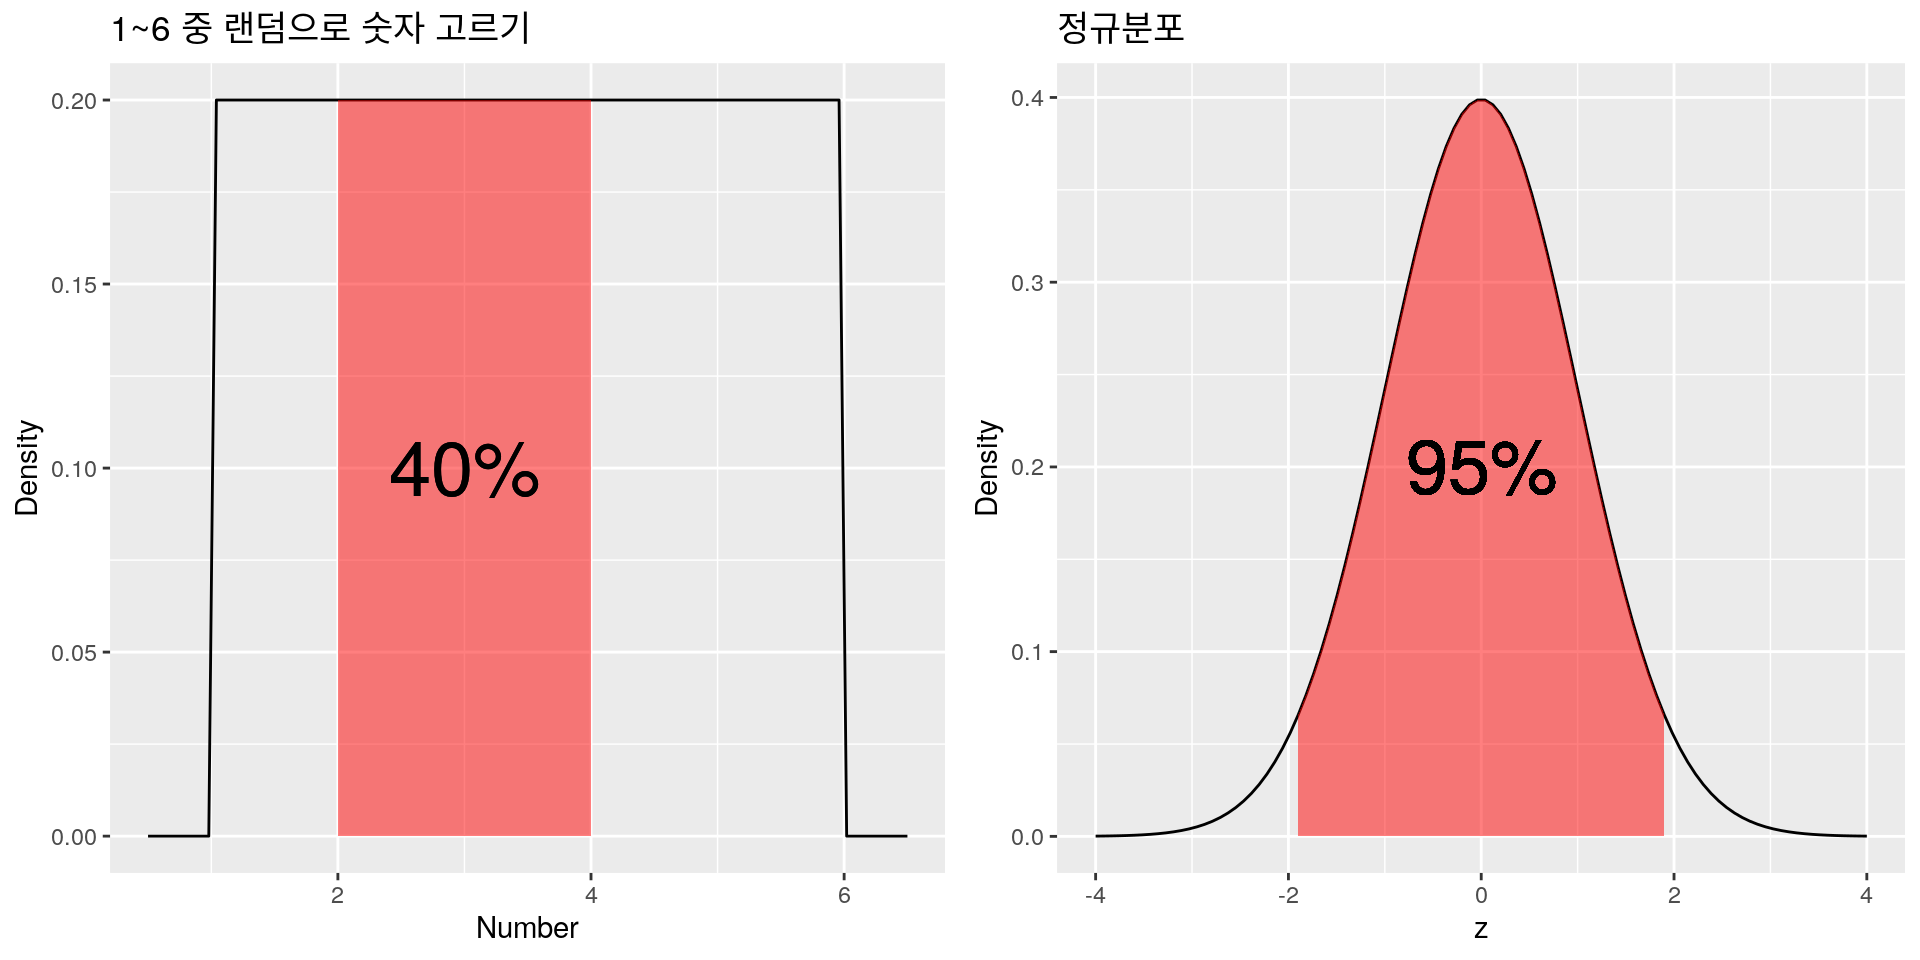
\includegraphics{Basic-stat_files/figure-latex/unnamed-chunk-4-1} 

}

\caption{연속 사건의 확률 예시}\label{fig:unnamed-chunk-4}
\end{figure}

정리하자면 \textbf{연속사건의 경우에는 특정 사건이 일어날 확률은 모두 0이며, 어떤 구간에 속할 확률은 PDF를 이용해서 구할 수 있다}고 할 수 있다. 그러면 특정 사건에 대한 해석은 할 수 없는 것인가? 순순히 할 수 없다고 말하기는 아쉽다. 위의 정규분포의 경우를 보면 0이 나올 확률도 0, 1이 나올 확률도 0, 999가 나올 확률도 0으로 모두 같으므로 0, 1, 999가 나올 가능성은 전혀 차이가 없다고 말해야 한다. 그러나 우리 모두는 정규분포의 그림을 보고 직관적으로 느끼고 있다. 가장 위로 솟아올라 있는 0 근처가 나올 가능성이 가장 높고, 1 근처가 나올 가능성은 그보다 낮으며, 999같이 큰 수가 나올 가능성은 거의 없다는 것을\ldots{} 그러나 확률이라는 지표로는 이런 연속사건간의 가능성 차이를 표시할 수가 없다는 문제가 있다.

\hypertarget{uxd2b9uxc815-uxc0acuxac74uxc774-uxc77cuxc5b4uxb0a0-uxac00uxb2a5uxc131uxc744-uxbe44uxad50uxd560-uxc218uxb294-uxc5c6uxc744uxae4c-uxac00uxb2a5uxb3c4likelihood}{%
\section{특정 사건이 일어날 가능성을 비교할 수는 없을까?: 가능도(Likelihood)}\label{uxd2b9uxc815-uxc0acuxac74uxc774-uxc77cuxc5b4uxb0a0-uxac00uxb2a5uxc131uxc744-uxbe44uxad50uxd560-uxc218uxb294-uxc5c6uxc744uxae4c-uxac00uxb2a5uxb3c4likelihood}}

방금 설명한 대로 연속사건에서는 특정 사건이 일어날 확률이 전부 0으로 계산되기 때문에 사건들이 일어날 가능성을 비교하는 것이 불가능하며, \textbf{가능도}라는 개념을 적용해야 이를 비교할 수 있다. 그러나 지금 가능도의 엄밀한 정의를 설명하는 것은 이해를 돕는데 도움이 안될 것이며, 직관적인 설명을 이용할 것인데, 쉽게 말하자면 \textbf{위에 있는 그래프들에서 \(y\)값}을 가능도로 생각하면 된다. 즉, \textbf{\(y\)값이 높을수록 일어날 가능성이 높은 사건}이라는 것이다. 주사위나 동전을 던지는 경우는 \(y\)값이 각 사건이 일어날 확률을 나타내었으므로 가능도=확률이 되어, 확률이 높을수록 일어날 가능성이 높은 사건이 된다. 한편 정규분포같이 연속사건인 경우는 PDF의 값이 바로 \(y\)가 되며 0에 해당하는 PDF값이 0.4로 1 에 해당하는 PDF값인 0.24보다 높아 0 근처의 숫자가 나올 가능성이 1 근처의 숫자가 나올 가능성보다 높다고 할 수 있으며, 0이 나올 확률과 1이 나올 확률이 모두 0인 것과는 대조적이다. 이를 정리하면 가능도의 직관적인 정의는 다음과 같다.

\begin{itemize}
\tightlist
\item
  가능도의 직관적인 정의 : 확률분포함수의 \(y\)값

  \begin{itemize}
  \tightlist
  \item
    셀 수 있는 사건: \textbf{가능도 = 확률}
  \item
    연속 사건: \textbf{가능도 \(\neq\) 확률, 가능도 = PDF값}
  \end{itemize}
\end{itemize}

\hypertarget{uxc0acuxac74uxc774-uxc5ecuxb7ec-uxbc88-uxc77cuxc5b4uxb0a0-uxacbduxc6b0uxc5d0uxc11cuxc758-uxac00uxb2a5uxb3c4}{%
\section{사건이 여러 번 일어날 경우에서의 가능도}\label{uxc0acuxac74uxc774-uxc5ecuxb7ec-uxbc88-uxc77cuxc5b4uxb0a0-uxacbduxc6b0uxc5d0uxc11cuxc758-uxac00uxb2a5uxb3c4}}

이번에는 사건이 여러 번 일어날 경우를 생각해 보자. 먼저 아래의 두 문제를 풀어보자.

\begin{enumerate}
\def\labelenumi{\arabic{enumi}.}
\tightlist
\item
  주사위를 3번 던져 각각 1,3,6이 나올 확률은 얼마일까?
\item
  동전을 10번 던지는 일을 3회 시행하여 앞면이 각각 2,5,7번 나올 확률은 얼마일까?
\end{enumerate}

1번의 경우 주사위를 던져 1,3,6이 나올 확률은 전부 \(\frac{1}{6}\)이므로 정답은 \(\frac{1}{6}\times\frac{1}{6}\times\frac{1}{6}=\frac{1}{216}\)이고, 2번의 경우 동전을 10번 던져 앞면이 2,5,7번 나올 확률은 앞에서와 같이 각각 0.044, 0.246, 0.117이므로 정답은 0.044 \(\times\) 0.246 \(\times\) 0.117\(=\) 0.001이다. 가능도도 마찬가지이다. 앞서 \textbf{셀 수 있는 사건에서는 확률과 가능도가 같다}고 했으므로 주사위를 3번 던져 각각 1,3,6 이 나올 가능성을 나타내는 가능도는 \(\frac{1}{216}\)이 되고, 동전을 던지는 경우의 가능도도 마찬가지로 확률과
같은 0.001이 된다. 이제 연속사건이 여러 번 일어날 경우를 살펴보자. 앞서 언급한 평균 0, 분산 1인 정규분포에서 숫자를 3번 뽑았을 때 차례대로 -1,0,1이 나올 확률은 각각의 사건이 일어날 확률이 모두 0이므로 결국 0이 된다. 그러나 가능도의 경우 -1,1이 나올 가능도는 0.24, 0이 나올 가능도는 0.4이므로 -1,0,1이 나올 가능도는 0.24 \(\times\) 0.4 \(\times\) 0.24 \(=\) 0.02가 되어 확률과는 다른 값으로 나타나게 된다.

\hypertarget{uxc9c4uxc2e4uxc744-uxcc3euxb294-uxbc29uxbc95-uxcd5cuxb300uxac00uxb2a5uxb3c4-uxcd94uxc815uxb7c9maximum-likelihood-estimator-mle}{%
\section{진실을 찾는 방법: 최대가능도 추정량(Maximum Likelihood Estimator, MLE)}\label{uxc9c4uxc2e4uxc744-uxcc3euxb294-uxbc29uxbc95-uxcd5cuxb300uxac00uxb2a5uxb3c4-uxcd94uxc815uxb7c9maximum-likelihood-estimator-mle}}

가능도 관련 마지막 주제로 최대 가능도 추정량(이하 MLE)에 대해 알아보겠다. MLE는 기초적인 통계분석에서 회귀분석에 이르기까지 거의 모든 통계분석에서 참값을 추정하는 원리이지만, 설명의 어려움 때문인지 거의 모든 기초통계 교과서에서 설명이 빠져 있다. 여기서는 두 가지 예를 가지고 MLE의 개념에 대해 설명할 것인데 먼저 모양이 변형된 동전을 생각해 보자.

\hypertarget{uxc6081-uxbaa8uxc591uxc774-uxc77cuxadf8uxb7ecuxc9c4-uxb3d9uxc804}{%
\subsection{예1: 모양이 일그러진 동전}\label{uxc6081-uxbaa8uxc591uxc774-uxc77cuxadf8uxb7ecuxc9c4-uxb3d9uxc804}}

지금까지와는 다르게 이 동전은 모양이 많이 일그러져서 앞이 나올 확률이 0.5라고 말할 수가 없고, 실제로 던져봐야 그 확률을 알 수 있을 것 같다. 실제로 1000번을 던져봤더니 앞이 400번, 뒤가 600번 나왔다면 우리는 동전을 던져 앞이 나올 확률 \(p\)가 대략 얼마 정도라고 생각할까? 아마 대부분은 0.4정도라고 생각할 것이며 이것은 \(p\)의 MLE값과 일치한다. 풀어서 설명하면 \textbf{동전을 1000번 던져서 앞이 400번 나올 가능성을 최대로 하는 \(p\)는 0.4}라는 뜻이며 수식을 이용한 엄밀한 증명은 다음과 같다.

\begin{enumerate}
\def\labelenumi{\arabic{enumi}.}
\tightlist
\item
  앞면이 나올 확률이 \(p\)라면 1000번을 던져 앞이 400번, 뒤가 600번 나올 가능도(=확률) \(L=_{1000} C_{400}p^{400}(1-p)^{600}\)이다. 수식이 싫으면 이 \(L\)이 최대값을 가지는 \(p\)를 계산해보면 0.4가 나온다는 것을 인정하고 그냥 넘어가자.
\item
  \(L\)이 언제 최대가 되는지 살펴보자. \(L\)이 최대가 되는 것은 \(p^{400}(1-p)^{600}\)가 최대가 될 때인데 산술-기하 평균 부등식에 의하여 \(600= \frac{3}{2}p\times 400 + (1-p)\times 600 \ge 1000\times \{(\frac{3}{2}p)^{400}(1-p)^{600}\}^{\frac{1}{1000}}\)이 된다.\\
\item
  따라서 \(p^{400}(1-p)^{600}\)의 최대값은 \((\frac{600}{1000})^{1000} \times (\frac{2}{3})^{400}\)이 되며,
\item
  \(L\)이 최대값이 될 때는 앞의 산술-기하평균 부등식의 등호조건이 성립할 때이므로 \(\frac{3}{2}p=1-p\) 즉, \(p=0.4\)가 된다.
\end{enumerate}

더 직관적으로 이해해보기 위해 앞면이 나올 확률 \(p\)에 따른 가능도 \(L\)의 값을 그래프로 그려보면 아래와 같다.

\begin{figure}

{\centering 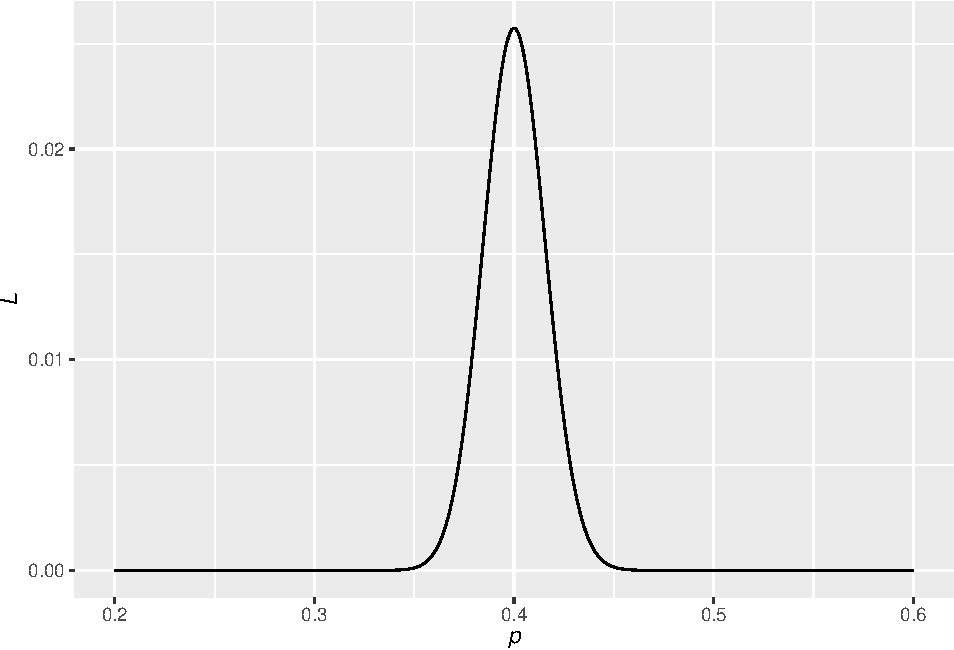
\includegraphics{Basic-stat_files/figure-latex/unnamed-chunk-5-1} 

}

\caption{앞면이 나올 확률 $p$에 따른 가능도 $L$의 값}\label{fig:unnamed-chunk-5}
\end{figure}

그림으로 살펴봐도 \(p\)가 0.4일 때 \(L\)의 값이 최대임을 알 수 있다. 지금까지 이야기를 다시 한 번 정리 해 보자. 동전을 1000번 던져 앞이 400번, 뒤가 600번 나왔다면 우리는 직관적으로 앞이 나올 확률 \(p\)는 0.4 정도라고 생각할 것이며, 실제 이런 일이 발생할 가능성을 최대로 하는 \(p\)를 계산하면 0.4가 된다. 이를 간략히 \textbf{\(p\)의 MLE는 0.4}라고 표현한다. 즉, MLE는 우리의 가능성과 확률에 대한 직관을 수리적으로 표현한 것에 불과하며 어렵게 생각할 필요가 없다고 말하고 싶다.

\hypertarget{uxc6082-uxb098uxc758-uxc2e4uxc81c-uxd0a4}{%
\subsection{예2: 나의 실제 키}\label{uxc6082-uxb098uxc758-uxc2e4uxc81c-uxd0a4}}

새로운 예시로 나의 키를 재는 상황을 생각해 보자. 키는 재는 시간, 방법에 따라서 실제 키와 조금씩 오차가 있을 수 밖에 없다. 만약 키를 5번 측정해서 178,179,180,181,182(cm)가 나왔다면 나의 실제 키는 얼마일까? 물론 많은 사람들이 가장 높게 나온 182cm을 자기 실제 키라고 생각할 수 있겠지만\ldots{} 합리적(?)인 사람이라면 아마 다섯 번의 평균인 180cm을 실제 자신의 키라고 생각할 것이다. 그렇다면 키의 MLE 값은 얼마일까? 즉, \textbf{키를 5번 측정했을 때 178,179,180,181,182cm이 나올 가능성이 최대가 되는 나의 키는 얼마일까?} 일그러진 동전 때와 마찬가지로 직관과 MLE는 일치할까? 이제부터 나의 키의 MLE값을 계산할 것인데 그 전에 한 가지 가정을 하려고 한다. 그것은 바로 \textbf{키의 측정값은 참값을 평균으로 하는 정규분포를 따른다}는 것이다. 키의 측정값은 어떤 값이든 갖을 수 있으며 오차가 적은 값이 오차가 큰 값보다 나올 가능성이 높다는 점으로 생각해 볼 때, 정규분포를 따른다는 가정은 큰 무리가 없을 것 같다. 이 가정 하에서 키의 MLE를 구하는 과정은 다음과 같다. 아까와 마찬가지로 수식이 싫은 사람은 바로 그림으로 내려가 직관적으로 이해하길 바란다.

\begin{enumerate}
\def\labelenumi{\arabic{enumi}.}
\tightlist
\item
  키의 참값이 \(\mu\)일 때 측정값은 평균 \(\mu\), 분산 \(\sigma^2\)인 정규분포를 따른다.
\item
  키의 측정값이 \(x\)일 때의 가능도, 즉 정규분포의 \(y\)값은 \(\frac{1}{\sqrt{2\pi}\sigma}e^{-\frac{(x-\mu)^2}{2\sigma^2}}\)이다.
\item
  5번 측정한 키가 178,179,180,181,182가 나올 가능도 \(L\)은 각각의 가능도의 곱인 \(\frac{1}{\sqrt{2\pi}\sigma^2}e^{-\frac{(178-\mu)^2}{2\sigma^2}}\times\frac{1}{\sqrt{2\pi}\sigma^2}e^{-\frac{(179-\mu)^2}{2\sigma^2}}\times\frac{1}{\sqrt{2\pi}\sigma^2}e^{-\frac{(180-\mu)^2}{2\sigma^2}}\times\frac{1}{\sqrt{2\pi}\sigma^2}e^{-\frac{(181-\mu)^2}{2\sigma^2}}\times\frac{1}{\sqrt{2\pi}\sigma^2}e^{-\frac{(182-\mu)^2}{2\sigma^2}}\)이다.
\item
  \(L\)이 최대가 된다는 것은 \(e^{-\frac{(178-\mu)^2}{2\sigma^2}}\times e^{-\frac{(179-\mu)^2}{2\sigma^2}}\times e^{-\frac{(180-\mu)^2}{2\sigma^2}}\times e^{-\frac{(181-\mu)^2}{2\sigma^2}}\times e^{-\frac{(182-\mu)^2}{2\sigma^2}}\) \(=\) \(e^{-(\frac{(178-\mu)^2+(179-\mu)^2+(180-\mu)^2+(181-\mu)^2+(182-\mu)^2}{2\sigma^2})}\)가 최대가 된다는 뜻이고, 이는 다시 \((178-\mu)^2+(179-\mu)^2+(180-\mu)^2+(181-\mu)^2+(182-\mu)^2\)가 최소가 되는 것으로 해석할 수 있다.
\item
  \((178-\mu)^2+(179-\mu)^2+(180-\mu)^2+(181-\mu)^2+(182-\mu)^2\)은 \(\mu=180\)에서 최소값을 가짐을 쉽게 알 수 있고, 따라서 \(\mu\)의 MLE는 180이다.
\end{enumerate}

이번에도 직관적인 이해를 위해 \(\sigma^2=1\)로 가정한 후, 실제 키인 \(\mu\)와 그에 해당하는 가능도 \(L\)의 그래프를 살펴보자.

\begin{verbatim}
## Warning in grid.Call(C_textBounds, as.graphicsAnnot(x$label), x$x, x$y, :
## font metrics unknown for Unicode character U+c2e4
\end{verbatim}

\begin{verbatim}
## Warning in grid.Call(C_textBounds, as.graphicsAnnot(x$label), x$x, x$y, :
## font metrics unknown for Unicode character U+c81c
\end{verbatim}

\begin{verbatim}
## Warning in grid.Call(C_textBounds, as.graphicsAnnot(x$label), x$x, x$y, :
## font metrics unknown for Unicode character U+d0a4
\end{verbatim}

\begin{verbatim}
## Warning in grid.Call(C_textBounds, as.graphicsAnnot(x$label), x$x, x$y, :
## conversion failure on '실제 키(' in 'mbcsToSbcs': dot substituted for <ec>
\end{verbatim}

\begin{verbatim}
## Warning in grid.Call(C_textBounds, as.graphicsAnnot(x$label), x$x, x$y, :
## conversion failure on '실제 키(' in 'mbcsToSbcs': dot substituted for <8b>
\end{verbatim}

\begin{verbatim}
## Warning in grid.Call(C_textBounds, as.graphicsAnnot(x$label), x$x, x$y, :
## conversion failure on '실제 키(' in 'mbcsToSbcs': dot substituted for <a4>
\end{verbatim}

\begin{verbatim}
## Warning in grid.Call(C_textBounds, as.graphicsAnnot(x$label), x$x, x$y, :
## conversion failure on '실제 키(' in 'mbcsToSbcs': dot substituted for <ec>
\end{verbatim}

\begin{verbatim}
## Warning in grid.Call(C_textBounds, as.graphicsAnnot(x$label), x$x, x$y, :
## conversion failure on '실제 키(' in 'mbcsToSbcs': dot substituted for <a0>
\end{verbatim}

\begin{verbatim}
## Warning in grid.Call(C_textBounds, as.graphicsAnnot(x$label), x$x, x$y, :
## conversion failure on '실제 키(' in 'mbcsToSbcs': dot substituted for <9c>
\end{verbatim}

\begin{verbatim}
## Warning in grid.Call(C_textBounds, as.graphicsAnnot(x$label), x$x, x$y, :
## conversion failure on '실제 키(' in 'mbcsToSbcs': dot substituted for <ed>
\end{verbatim}

\begin{verbatim}
## Warning in grid.Call(C_textBounds, as.graphicsAnnot(x$label), x$x, x$y, :
## conversion failure on '실제 키(' in 'mbcsToSbcs': dot substituted for <82>
\end{verbatim}

\begin{verbatim}
## Warning in grid.Call(C_textBounds, as.graphicsAnnot(x$label), x$x, x$y, :
## conversion failure on '실제 키(' in 'mbcsToSbcs': dot substituted for <a4>
\end{verbatim}

\begin{verbatim}
## Warning in grid.Call(C_textBounds, as.graphicsAnnot(x$label), x$x, x$y, :
## font metrics unknown for Unicode character U+c2e4
\end{verbatim}

\begin{verbatim}
## Warning in grid.Call(C_textBounds, as.graphicsAnnot(x$label), x$x, x$y, :
## font metrics unknown for Unicode character U+c81c
\end{verbatim}

\begin{verbatim}
## Warning in grid.Call(C_textBounds, as.graphicsAnnot(x$label), x$x, x$y, :
## font metrics unknown for Unicode character U+d0a4
\end{verbatim}

\begin{verbatim}
## Warning in grid.Call(C_textBounds, as.graphicsAnnot(x$label), x$x, x$y, :
## conversion failure on '실제 키(' in 'mbcsToSbcs': dot substituted for <ec>
\end{verbatim}

\begin{verbatim}
## Warning in grid.Call(C_textBounds, as.graphicsAnnot(x$label), x$x, x$y, :
## conversion failure on '실제 키(' in 'mbcsToSbcs': dot substituted for <8b>
\end{verbatim}

\begin{verbatim}
## Warning in grid.Call(C_textBounds, as.graphicsAnnot(x$label), x$x, x$y, :
## conversion failure on '실제 키(' in 'mbcsToSbcs': dot substituted for <a4>
\end{verbatim}

\begin{verbatim}
## Warning in grid.Call(C_textBounds, as.graphicsAnnot(x$label), x$x, x$y, :
## conversion failure on '실제 키(' in 'mbcsToSbcs': dot substituted for <ec>
\end{verbatim}

\begin{verbatim}
## Warning in grid.Call(C_textBounds, as.graphicsAnnot(x$label), x$x, x$y, :
## conversion failure on '실제 키(' in 'mbcsToSbcs': dot substituted for <a0>
\end{verbatim}

\begin{verbatim}
## Warning in grid.Call(C_textBounds, as.graphicsAnnot(x$label), x$x, x$y, :
## conversion failure on '실제 키(' in 'mbcsToSbcs': dot substituted for <9c>
\end{verbatim}

\begin{verbatim}
## Warning in grid.Call(C_textBounds, as.graphicsAnnot(x$label), x$x, x$y, :
## conversion failure on '실제 키(' in 'mbcsToSbcs': dot substituted for <ed>
\end{verbatim}

\begin{verbatim}
## Warning in grid.Call(C_textBounds, as.graphicsAnnot(x$label), x$x, x$y, :
## conversion failure on '실제 키(' in 'mbcsToSbcs': dot substituted for <82>
\end{verbatim}

\begin{verbatim}
## Warning in grid.Call(C_textBounds, as.graphicsAnnot(x$label), x$x, x$y, :
## conversion failure on '실제 키(' in 'mbcsToSbcs': dot substituted for <a4>
\end{verbatim}

\begin{verbatim}
## Warning in grid.Call(C_textBounds, as.graphicsAnnot(x$label), x$x, x$y, :
## font metrics unknown for Unicode character U+c2e4
\end{verbatim}

\begin{verbatim}
## Warning in grid.Call(C_textBounds, as.graphicsAnnot(x$label), x$x, x$y, :
## font metrics unknown for Unicode character U+c81c
\end{verbatim}

\begin{verbatim}
## Warning in grid.Call(C_textBounds, as.graphicsAnnot(x$label), x$x, x$y, :
## font metrics unknown for Unicode character U+d0a4
\end{verbatim}

\begin{verbatim}
## Warning in grid.Call(C_textBounds, as.graphicsAnnot(x$label), x$x, x$y, :
## conversion failure on '실제 키(' in 'mbcsToSbcs': dot substituted for <ec>
\end{verbatim}

\begin{verbatim}
## Warning in grid.Call(C_textBounds, as.graphicsAnnot(x$label), x$x, x$y, :
## conversion failure on '실제 키(' in 'mbcsToSbcs': dot substituted for <8b>
\end{verbatim}

\begin{verbatim}
## Warning in grid.Call(C_textBounds, as.graphicsAnnot(x$label), x$x, x$y, :
## conversion failure on '실제 키(' in 'mbcsToSbcs': dot substituted for <a4>
\end{verbatim}

\begin{verbatim}
## Warning in grid.Call(C_textBounds, as.graphicsAnnot(x$label), x$x, x$y, :
## conversion failure on '실제 키(' in 'mbcsToSbcs': dot substituted for <ec>
\end{verbatim}

\begin{verbatim}
## Warning in grid.Call(C_textBounds, as.graphicsAnnot(x$label), x$x, x$y, :
## conversion failure on '실제 키(' in 'mbcsToSbcs': dot substituted for <a0>
\end{verbatim}

\begin{verbatim}
## Warning in grid.Call(C_textBounds, as.graphicsAnnot(x$label), x$x, x$y, :
## conversion failure on '실제 키(' in 'mbcsToSbcs': dot substituted for <9c>
\end{verbatim}

\begin{verbatim}
## Warning in grid.Call(C_textBounds, as.graphicsAnnot(x$label), x$x, x$y, :
## conversion failure on '실제 키(' in 'mbcsToSbcs': dot substituted for <ed>
\end{verbatim}

\begin{verbatim}
## Warning in grid.Call(C_textBounds, as.graphicsAnnot(x$label), x$x, x$y, :
## conversion failure on '실제 키(' in 'mbcsToSbcs': dot substituted for <82>
\end{verbatim}

\begin{verbatim}
## Warning in grid.Call(C_textBounds, as.graphicsAnnot(x$label), x$x, x$y, :
## conversion failure on '실제 키(' in 'mbcsToSbcs': dot substituted for <a4>
\end{verbatim}

\begin{verbatim}
## Warning in grid.Call(C_textBounds, as.graphicsAnnot(x$label), x$x, x$y, :
## font metrics unknown for Unicode character U+c2e4
\end{verbatim}

\begin{verbatim}
## Warning in grid.Call(C_textBounds, as.graphicsAnnot(x$label), x$x, x$y, :
## font metrics unknown for Unicode character U+c81c
\end{verbatim}

\begin{verbatim}
## Warning in grid.Call(C_textBounds, as.graphicsAnnot(x$label), x$x, x$y, :
## font metrics unknown for Unicode character U+d0a4
\end{verbatim}

\begin{verbatim}
## Warning in grid.Call(C_textBounds, as.graphicsAnnot(x$label), x$x, x$y, :
## conversion failure on '실제 키(' in 'mbcsToSbcs': dot substituted for <ec>
\end{verbatim}

\begin{verbatim}
## Warning in grid.Call(C_textBounds, as.graphicsAnnot(x$label), x$x, x$y, :
## conversion failure on '실제 키(' in 'mbcsToSbcs': dot substituted for <8b>
\end{verbatim}

\begin{verbatim}
## Warning in grid.Call(C_textBounds, as.graphicsAnnot(x$label), x$x, x$y, :
## conversion failure on '실제 키(' in 'mbcsToSbcs': dot substituted for <a4>
\end{verbatim}

\begin{verbatim}
## Warning in grid.Call(C_textBounds, as.graphicsAnnot(x$label), x$x, x$y, :
## conversion failure on '실제 키(' in 'mbcsToSbcs': dot substituted for <ec>
\end{verbatim}

\begin{verbatim}
## Warning in grid.Call(C_textBounds, as.graphicsAnnot(x$label), x$x, x$y, :
## conversion failure on '실제 키(' in 'mbcsToSbcs': dot substituted for <a0>
\end{verbatim}

\begin{verbatim}
## Warning in grid.Call(C_textBounds, as.graphicsAnnot(x$label), x$x, x$y, :
## conversion failure on '실제 키(' in 'mbcsToSbcs': dot substituted for <9c>
\end{verbatim}

\begin{verbatim}
## Warning in grid.Call(C_textBounds, as.graphicsAnnot(x$label), x$x, x$y, :
## conversion failure on '실제 키(' in 'mbcsToSbcs': dot substituted for <ed>
\end{verbatim}

\begin{verbatim}
## Warning in grid.Call(C_textBounds, as.graphicsAnnot(x$label), x$x, x$y, :
## conversion failure on '실제 키(' in 'mbcsToSbcs': dot substituted for <82>
\end{verbatim}

\begin{verbatim}
## Warning in grid.Call(C_textBounds, as.graphicsAnnot(x$label), x$x, x$y, :
## conversion failure on '실제 키(' in 'mbcsToSbcs': dot substituted for <a4>
\end{verbatim}

\begin{verbatim}
## Warning in grid.Call(C_textBounds, as.graphicsAnnot(x$label), x$x, x$y, :
## font metrics unknown for Unicode character U+c2e4
\end{verbatim}

\begin{verbatim}
## Warning in grid.Call(C_textBounds, as.graphicsAnnot(x$label), x$x, x$y, :
## font metrics unknown for Unicode character U+c81c
\end{verbatim}

\begin{verbatim}
## Warning in grid.Call(C_textBounds, as.graphicsAnnot(x$label), x$x, x$y, :
## font metrics unknown for Unicode character U+d0a4
\end{verbatim}

\begin{verbatim}
## Warning in grid.Call(C_textBounds, as.graphicsAnnot(x$label), x$x, x$y, :
## conversion failure on '실제 키(' in 'mbcsToSbcs': dot substituted for <ec>
\end{verbatim}

\begin{verbatim}
## Warning in grid.Call(C_textBounds, as.graphicsAnnot(x$label), x$x, x$y, :
## conversion failure on '실제 키(' in 'mbcsToSbcs': dot substituted for <8b>
\end{verbatim}

\begin{verbatim}
## Warning in grid.Call(C_textBounds, as.graphicsAnnot(x$label), x$x, x$y, :
## conversion failure on '실제 키(' in 'mbcsToSbcs': dot substituted for <a4>
\end{verbatim}

\begin{verbatim}
## Warning in grid.Call(C_textBounds, as.graphicsAnnot(x$label), x$x, x$y, :
## conversion failure on '실제 키(' in 'mbcsToSbcs': dot substituted for <ec>
\end{verbatim}

\begin{verbatim}
## Warning in grid.Call(C_textBounds, as.graphicsAnnot(x$label), x$x, x$y, :
## conversion failure on '실제 키(' in 'mbcsToSbcs': dot substituted for <a0>
\end{verbatim}

\begin{verbatim}
## Warning in grid.Call(C_textBounds, as.graphicsAnnot(x$label), x$x, x$y, :
## conversion failure on '실제 키(' in 'mbcsToSbcs': dot substituted for <9c>
\end{verbatim}

\begin{verbatim}
## Warning in grid.Call(C_textBounds, as.graphicsAnnot(x$label), x$x, x$y, :
## conversion failure on '실제 키(' in 'mbcsToSbcs': dot substituted for <ed>
\end{verbatim}

\begin{verbatim}
## Warning in grid.Call(C_textBounds, as.graphicsAnnot(x$label), x$x, x$y, :
## conversion failure on '실제 키(' in 'mbcsToSbcs': dot substituted for <82>
\end{verbatim}

\begin{verbatim}
## Warning in grid.Call(C_textBounds, as.graphicsAnnot(x$label), x$x, x$y, :
## conversion failure on '실제 키(' in 'mbcsToSbcs': dot substituted for <a4>
\end{verbatim}

\begin{verbatim}
## Warning in grid.Call(C_textBounds, as.graphicsAnnot(x$label), x$x, x$y, :
## font metrics unknown for Unicode character U+c2e4
\end{verbatim}

\begin{verbatim}
## Warning in grid.Call(C_textBounds, as.graphicsAnnot(x$label), x$x, x$y, :
## font metrics unknown for Unicode character U+c81c
\end{verbatim}

\begin{verbatim}
## Warning in grid.Call(C_textBounds, as.graphicsAnnot(x$label), x$x, x$y, :
## font metrics unknown for Unicode character U+d0a4
\end{verbatim}

\begin{verbatim}
## Warning in grid.Call(C_textBounds, as.graphicsAnnot(x$label), x$x, x$y, :
## conversion failure on '실제 키(' in 'mbcsToSbcs': dot substituted for <ec>
\end{verbatim}

\begin{verbatim}
## Warning in grid.Call(C_textBounds, as.graphicsAnnot(x$label), x$x, x$y, :
## conversion failure on '실제 키(' in 'mbcsToSbcs': dot substituted for <8b>
\end{verbatim}

\begin{verbatim}
## Warning in grid.Call(C_textBounds, as.graphicsAnnot(x$label), x$x, x$y, :
## conversion failure on '실제 키(' in 'mbcsToSbcs': dot substituted for <a4>
\end{verbatim}

\begin{verbatim}
## Warning in grid.Call(C_textBounds, as.graphicsAnnot(x$label), x$x, x$y, :
## conversion failure on '실제 키(' in 'mbcsToSbcs': dot substituted for <ec>
\end{verbatim}

\begin{verbatim}
## Warning in grid.Call(C_textBounds, as.graphicsAnnot(x$label), x$x, x$y, :
## conversion failure on '실제 키(' in 'mbcsToSbcs': dot substituted for <a0>
\end{verbatim}

\begin{verbatim}
## Warning in grid.Call(C_textBounds, as.graphicsAnnot(x$label), x$x, x$y, :
## conversion failure on '실제 키(' in 'mbcsToSbcs': dot substituted for <9c>
\end{verbatim}

\begin{verbatim}
## Warning in grid.Call(C_textBounds, as.graphicsAnnot(x$label), x$x, x$y, :
## conversion failure on '실제 키(' in 'mbcsToSbcs': dot substituted for <ed>
\end{verbatim}

\begin{verbatim}
## Warning in grid.Call(C_textBounds, as.graphicsAnnot(x$label), x$x, x$y, :
## conversion failure on '실제 키(' in 'mbcsToSbcs': dot substituted for <82>
\end{verbatim}

\begin{verbatim}
## Warning in grid.Call(C_textBounds, as.graphicsAnnot(x$label), x$x, x$y, :
## conversion failure on '실제 키(' in 'mbcsToSbcs': dot substituted for <a4>
\end{verbatim}

\begin{verbatim}
## Warning in grid.Call(C_textBounds, as.graphicsAnnot(x$label), x$x, x$y, :
## font metrics unknown for Unicode character U+c2e4
\end{verbatim}

\begin{verbatim}
## Warning in grid.Call(C_textBounds, as.graphicsAnnot(x$label), x$x, x$y, :
## font metrics unknown for Unicode character U+c81c
\end{verbatim}

\begin{verbatim}
## Warning in grid.Call(C_textBounds, as.graphicsAnnot(x$label), x$x, x$y, :
## font metrics unknown for Unicode character U+d0a4
\end{verbatim}

\begin{verbatim}
## Warning in grid.Call(C_textBounds, as.graphicsAnnot(x$label), x$x, x$y, :
## conversion failure on '실제 키(' in 'mbcsToSbcs': dot substituted for <ec>
\end{verbatim}

\begin{verbatim}
## Warning in grid.Call(C_textBounds, as.graphicsAnnot(x$label), x$x, x$y, :
## conversion failure on '실제 키(' in 'mbcsToSbcs': dot substituted for <8b>
\end{verbatim}

\begin{verbatim}
## Warning in grid.Call(C_textBounds, as.graphicsAnnot(x$label), x$x, x$y, :
## conversion failure on '실제 키(' in 'mbcsToSbcs': dot substituted for <a4>
\end{verbatim}

\begin{verbatim}
## Warning in grid.Call(C_textBounds, as.graphicsAnnot(x$label), x$x, x$y, :
## conversion failure on '실제 키(' in 'mbcsToSbcs': dot substituted for <ec>
\end{verbatim}

\begin{verbatim}
## Warning in grid.Call(C_textBounds, as.graphicsAnnot(x$label), x$x, x$y, :
## conversion failure on '실제 키(' in 'mbcsToSbcs': dot substituted for <a0>
\end{verbatim}

\begin{verbatim}
## Warning in grid.Call(C_textBounds, as.graphicsAnnot(x$label), x$x, x$y, :
## conversion failure on '실제 키(' in 'mbcsToSbcs': dot substituted for <9c>
\end{verbatim}

\begin{verbatim}
## Warning in grid.Call(C_textBounds, as.graphicsAnnot(x$label), x$x, x$y, :
## conversion failure on '실제 키(' in 'mbcsToSbcs': dot substituted for <ed>
\end{verbatim}

\begin{verbatim}
## Warning in grid.Call(C_textBounds, as.graphicsAnnot(x$label), x$x, x$y, :
## conversion failure on '실제 키(' in 'mbcsToSbcs': dot substituted for <82>
\end{verbatim}

\begin{verbatim}
## Warning in grid.Call(C_textBounds, as.graphicsAnnot(x$label), x$x, x$y, :
## conversion failure on '실제 키(' in 'mbcsToSbcs': dot substituted for <a4>
\end{verbatim}

\begin{verbatim}
## Warning in grid.Call(C_textBounds, as.graphicsAnnot(x$label), x$x, x$y, :
## font metrics unknown for Unicode character U+c2e4
\end{verbatim}

\begin{verbatim}
## Warning in grid.Call(C_textBounds, as.graphicsAnnot(x$label), x$x, x$y, :
## font metrics unknown for Unicode character U+c81c
\end{verbatim}

\begin{verbatim}
## Warning in grid.Call(C_textBounds, as.graphicsAnnot(x$label), x$x, x$y, :
## font metrics unknown for Unicode character U+d0a4
\end{verbatim}

\begin{verbatim}
## Warning in grid.Call(C_textBounds, as.graphicsAnnot(x$label), x$x, x$y, :
## conversion failure on '실제 키(' in 'mbcsToSbcs': dot substituted for <ec>
\end{verbatim}

\begin{verbatim}
## Warning in grid.Call(C_textBounds, as.graphicsAnnot(x$label), x$x, x$y, :
## conversion failure on '실제 키(' in 'mbcsToSbcs': dot substituted for <8b>
\end{verbatim}

\begin{verbatim}
## Warning in grid.Call(C_textBounds, as.graphicsAnnot(x$label), x$x, x$y, :
## conversion failure on '실제 키(' in 'mbcsToSbcs': dot substituted for <a4>
\end{verbatim}

\begin{verbatim}
## Warning in grid.Call(C_textBounds, as.graphicsAnnot(x$label), x$x, x$y, :
## conversion failure on '실제 키(' in 'mbcsToSbcs': dot substituted for <ec>
\end{verbatim}

\begin{verbatim}
## Warning in grid.Call(C_textBounds, as.graphicsAnnot(x$label), x$x, x$y, :
## conversion failure on '실제 키(' in 'mbcsToSbcs': dot substituted for <a0>
\end{verbatim}

\begin{verbatim}
## Warning in grid.Call(C_textBounds, as.graphicsAnnot(x$label), x$x, x$y, :
## conversion failure on '실제 키(' in 'mbcsToSbcs': dot substituted for <9c>
\end{verbatim}

\begin{verbatim}
## Warning in grid.Call(C_textBounds, as.graphicsAnnot(x$label), x$x, x$y, :
## conversion failure on '실제 키(' in 'mbcsToSbcs': dot substituted for <ed>
\end{verbatim}

\begin{verbatim}
## Warning in grid.Call(C_textBounds, as.graphicsAnnot(x$label), x$x, x$y, :
## conversion failure on '실제 키(' in 'mbcsToSbcs': dot substituted for <82>
\end{verbatim}

\begin{verbatim}
## Warning in grid.Call(C_textBounds, as.graphicsAnnot(x$label), x$x, x$y, :
## conversion failure on '실제 키(' in 'mbcsToSbcs': dot substituted for <a4>
\end{verbatim}

\begin{verbatim}
## Warning in grid.Call(C_textBounds, as.graphicsAnnot(x$label), x$x, x$y, :
## font metrics unknown for Unicode character U+c2e4
\end{verbatim}

\begin{verbatim}
## Warning in grid.Call(C_textBounds, as.graphicsAnnot(x$label), x$x, x$y, :
## font metrics unknown for Unicode character U+c81c
\end{verbatim}

\begin{verbatim}
## Warning in grid.Call(C_textBounds, as.graphicsAnnot(x$label), x$x, x$y, :
## font metrics unknown for Unicode character U+d0a4
\end{verbatim}

\begin{verbatim}
## Warning in grid.Call(C_textBounds, as.graphicsAnnot(x$label), x$x, x$y, :
## conversion failure on '실제 키(' in 'mbcsToSbcs': dot substituted for <ec>
\end{verbatim}

\begin{verbatim}
## Warning in grid.Call(C_textBounds, as.graphicsAnnot(x$label), x$x, x$y, :
## conversion failure on '실제 키(' in 'mbcsToSbcs': dot substituted for <8b>
\end{verbatim}

\begin{verbatim}
## Warning in grid.Call(C_textBounds, as.graphicsAnnot(x$label), x$x, x$y, :
## conversion failure on '실제 키(' in 'mbcsToSbcs': dot substituted for <a4>
\end{verbatim}

\begin{verbatim}
## Warning in grid.Call(C_textBounds, as.graphicsAnnot(x$label), x$x, x$y, :
## conversion failure on '실제 키(' in 'mbcsToSbcs': dot substituted for <ec>
\end{verbatim}

\begin{verbatim}
## Warning in grid.Call(C_textBounds, as.graphicsAnnot(x$label), x$x, x$y, :
## conversion failure on '실제 키(' in 'mbcsToSbcs': dot substituted for <a0>
\end{verbatim}

\begin{verbatim}
## Warning in grid.Call(C_textBounds, as.graphicsAnnot(x$label), x$x, x$y, :
## conversion failure on '실제 키(' in 'mbcsToSbcs': dot substituted for <9c>
\end{verbatim}

\begin{verbatim}
## Warning in grid.Call(C_textBounds, as.graphicsAnnot(x$label), x$x, x$y, :
## conversion failure on '실제 키(' in 'mbcsToSbcs': dot substituted for <ed>
\end{verbatim}

\begin{verbatim}
## Warning in grid.Call(C_textBounds, as.graphicsAnnot(x$label), x$x, x$y, :
## conversion failure on '실제 키(' in 'mbcsToSbcs': dot substituted for <82>
\end{verbatim}

\begin{verbatim}
## Warning in grid.Call(C_textBounds, as.graphicsAnnot(x$label), x$x, x$y, :
## conversion failure on '실제 키(' in 'mbcsToSbcs': dot substituted for <a4>
\end{verbatim}

\begin{verbatim}
## Warning in grid.Call(C_textBounds, as.graphicsAnnot(x$label), x$x, x$y, :
## font metrics unknown for Unicode character U+c2e4
\end{verbatim}

\begin{verbatim}
## Warning in grid.Call(C_textBounds, as.graphicsAnnot(x$label), x$x, x$y, :
## font metrics unknown for Unicode character U+c81c
\end{verbatim}

\begin{verbatim}
## Warning in grid.Call(C_textBounds, as.graphicsAnnot(x$label), x$x, x$y, :
## font metrics unknown for Unicode character U+d0a4
\end{verbatim}

\begin{verbatim}
## Warning in grid.Call(C_textBounds, as.graphicsAnnot(x$label), x$x, x$y, :
## conversion failure on '실제 키(' in 'mbcsToSbcs': dot substituted for <ec>
\end{verbatim}

\begin{verbatim}
## Warning in grid.Call(C_textBounds, as.graphicsAnnot(x$label), x$x, x$y, :
## conversion failure on '실제 키(' in 'mbcsToSbcs': dot substituted for <8b>
\end{verbatim}

\begin{verbatim}
## Warning in grid.Call(C_textBounds, as.graphicsAnnot(x$label), x$x, x$y, :
## conversion failure on '실제 키(' in 'mbcsToSbcs': dot substituted for <a4>
\end{verbatim}

\begin{verbatim}
## Warning in grid.Call(C_textBounds, as.graphicsAnnot(x$label), x$x, x$y, :
## conversion failure on '실제 키(' in 'mbcsToSbcs': dot substituted for <ec>
\end{verbatim}

\begin{verbatim}
## Warning in grid.Call(C_textBounds, as.graphicsAnnot(x$label), x$x, x$y, :
## conversion failure on '실제 키(' in 'mbcsToSbcs': dot substituted for <a0>
\end{verbatim}

\begin{verbatim}
## Warning in grid.Call(C_textBounds, as.graphicsAnnot(x$label), x$x, x$y, :
## conversion failure on '실제 키(' in 'mbcsToSbcs': dot substituted for <9c>
\end{verbatim}

\begin{verbatim}
## Warning in grid.Call(C_textBounds, as.graphicsAnnot(x$label), x$x, x$y, :
## conversion failure on '실제 키(' in 'mbcsToSbcs': dot substituted for <ed>
\end{verbatim}

\begin{verbatim}
## Warning in grid.Call(C_textBounds, as.graphicsAnnot(x$label), x$x, x$y, :
## conversion failure on '실제 키(' in 'mbcsToSbcs': dot substituted for <82>
\end{verbatim}

\begin{verbatim}
## Warning in grid.Call(C_textBounds, as.graphicsAnnot(x$label), x$x, x$y, :
## conversion failure on '실제 키(' in 'mbcsToSbcs': dot substituted for <a4>
\end{verbatim}

\begin{verbatim}
## Warning in grid.Call(C_textBounds, as.graphicsAnnot(x$label), x$x, x$y, :
## font metrics unknown for Unicode character U+c2e4
\end{verbatim}

\begin{verbatim}
## Warning in grid.Call(C_textBounds, as.graphicsAnnot(x$label), x$x, x$y, :
## font metrics unknown for Unicode character U+c81c
\end{verbatim}

\begin{verbatim}
## Warning in grid.Call(C_textBounds, as.graphicsAnnot(x$label), x$x, x$y, :
## font metrics unknown for Unicode character U+d0a4
\end{verbatim}

\begin{verbatim}
## Warning in grid.Call(C_textBounds, as.graphicsAnnot(x$label), x$x, x$y, :
## conversion failure on '실제 키(' in 'mbcsToSbcs': dot substituted for <ec>
\end{verbatim}

\begin{verbatim}
## Warning in grid.Call(C_textBounds, as.graphicsAnnot(x$label), x$x, x$y, :
## conversion failure on '실제 키(' in 'mbcsToSbcs': dot substituted for <8b>
\end{verbatim}

\begin{verbatim}
## Warning in grid.Call(C_textBounds, as.graphicsAnnot(x$label), x$x, x$y, :
## conversion failure on '실제 키(' in 'mbcsToSbcs': dot substituted for <a4>
\end{verbatim}

\begin{verbatim}
## Warning in grid.Call(C_textBounds, as.graphicsAnnot(x$label), x$x, x$y, :
## conversion failure on '실제 키(' in 'mbcsToSbcs': dot substituted for <ec>
\end{verbatim}

\begin{verbatim}
## Warning in grid.Call(C_textBounds, as.graphicsAnnot(x$label), x$x, x$y, :
## conversion failure on '실제 키(' in 'mbcsToSbcs': dot substituted for <a0>
\end{verbatim}

\begin{verbatim}
## Warning in grid.Call(C_textBounds, as.graphicsAnnot(x$label), x$x, x$y, :
## conversion failure on '실제 키(' in 'mbcsToSbcs': dot substituted for <9c>
\end{verbatim}

\begin{verbatim}
## Warning in grid.Call(C_textBounds, as.graphicsAnnot(x$label), x$x, x$y, :
## conversion failure on '실제 키(' in 'mbcsToSbcs': dot substituted for <ed>
\end{verbatim}

\begin{verbatim}
## Warning in grid.Call(C_textBounds, as.graphicsAnnot(x$label), x$x, x$y, :
## conversion failure on '실제 키(' in 'mbcsToSbcs': dot substituted for <82>
\end{verbatim}

\begin{verbatim}
## Warning in grid.Call(C_textBounds, as.graphicsAnnot(x$label), x$x, x$y, :
## conversion failure on '실제 키(' in 'mbcsToSbcs': dot substituted for <a4>
\end{verbatim}

\begin{verbatim}
## Warning in grid.Call(C_textBounds, as.graphicsAnnot(x$label), x$x, x$y, :
## font metrics unknown for Unicode character U+c2e4
\end{verbatim}

\begin{verbatim}
## Warning in grid.Call(C_textBounds, as.graphicsAnnot(x$label), x$x, x$y, :
## font metrics unknown for Unicode character U+c81c
\end{verbatim}

\begin{verbatim}
## Warning in grid.Call(C_textBounds, as.graphicsAnnot(x$label), x$x, x$y, :
## font metrics unknown for Unicode character U+d0a4
\end{verbatim}

\begin{verbatim}
## Warning in grid.Call(C_textBounds, as.graphicsAnnot(x$label), x$x, x$y, :
## conversion failure on '실제 키(' in 'mbcsToSbcs': dot substituted for <ec>
\end{verbatim}

\begin{verbatim}
## Warning in grid.Call(C_textBounds, as.graphicsAnnot(x$label), x$x, x$y, :
## conversion failure on '실제 키(' in 'mbcsToSbcs': dot substituted for <8b>
\end{verbatim}

\begin{verbatim}
## Warning in grid.Call(C_textBounds, as.graphicsAnnot(x$label), x$x, x$y, :
## conversion failure on '실제 키(' in 'mbcsToSbcs': dot substituted for <a4>
\end{verbatim}

\begin{verbatim}
## Warning in grid.Call(C_textBounds, as.graphicsAnnot(x$label), x$x, x$y, :
## conversion failure on '실제 키(' in 'mbcsToSbcs': dot substituted for <ec>
\end{verbatim}

\begin{verbatim}
## Warning in grid.Call(C_textBounds, as.graphicsAnnot(x$label), x$x, x$y, :
## conversion failure on '실제 키(' in 'mbcsToSbcs': dot substituted for <a0>
\end{verbatim}

\begin{verbatim}
## Warning in grid.Call(C_textBounds, as.graphicsAnnot(x$label), x$x, x$y, :
## conversion failure on '실제 키(' in 'mbcsToSbcs': dot substituted for <9c>
\end{verbatim}

\begin{verbatim}
## Warning in grid.Call(C_textBounds, as.graphicsAnnot(x$label), x$x, x$y, :
## conversion failure on '실제 키(' in 'mbcsToSbcs': dot substituted for <ed>
\end{verbatim}

\begin{verbatim}
## Warning in grid.Call(C_textBounds, as.graphicsAnnot(x$label), x$x, x$y, :
## conversion failure on '실제 키(' in 'mbcsToSbcs': dot substituted for <82>
\end{verbatim}

\begin{verbatim}
## Warning in grid.Call(C_textBounds, as.graphicsAnnot(x$label), x$x, x$y, :
## conversion failure on '실제 키(' in 'mbcsToSbcs': dot substituted for <a4>
\end{verbatim}

\begin{verbatim}
## Warning in grid.Call(C_textBounds, as.graphicsAnnot(x$label), x$x, x$y, :
## font metrics unknown for Unicode character U+c2e4
\end{verbatim}

\begin{verbatim}
## Warning in grid.Call(C_textBounds, as.graphicsAnnot(x$label), x$x, x$y, :
## font metrics unknown for Unicode character U+c81c
\end{verbatim}

\begin{verbatim}
## Warning in grid.Call(C_textBounds, as.graphicsAnnot(x$label), x$x, x$y, :
## font metrics unknown for Unicode character U+d0a4
\end{verbatim}

\begin{verbatim}
## Warning in grid.Call(C_textBounds, as.graphicsAnnot(x$label), x$x, x$y, :
## conversion failure on '실제 키(' in 'mbcsToSbcs': dot substituted for <ec>
\end{verbatim}

\begin{verbatim}
## Warning in grid.Call(C_textBounds, as.graphicsAnnot(x$label), x$x, x$y, :
## conversion failure on '실제 키(' in 'mbcsToSbcs': dot substituted for <8b>
\end{verbatim}

\begin{verbatim}
## Warning in grid.Call(C_textBounds, as.graphicsAnnot(x$label), x$x, x$y, :
## conversion failure on '실제 키(' in 'mbcsToSbcs': dot substituted for <a4>
\end{verbatim}

\begin{verbatim}
## Warning in grid.Call(C_textBounds, as.graphicsAnnot(x$label), x$x, x$y, :
## conversion failure on '실제 키(' in 'mbcsToSbcs': dot substituted for <ec>
\end{verbatim}

\begin{verbatim}
## Warning in grid.Call(C_textBounds, as.graphicsAnnot(x$label), x$x, x$y, :
## conversion failure on '실제 키(' in 'mbcsToSbcs': dot substituted for <a0>
\end{verbatim}

\begin{verbatim}
## Warning in grid.Call(C_textBounds, as.graphicsAnnot(x$label), x$x, x$y, :
## conversion failure on '실제 키(' in 'mbcsToSbcs': dot substituted for <9c>
\end{verbatim}

\begin{verbatim}
## Warning in grid.Call(C_textBounds, as.graphicsAnnot(x$label), x$x, x$y, :
## conversion failure on '실제 키(' in 'mbcsToSbcs': dot substituted for <ed>
\end{verbatim}

\begin{verbatim}
## Warning in grid.Call(C_textBounds, as.graphicsAnnot(x$label), x$x, x$y, :
## conversion failure on '실제 키(' in 'mbcsToSbcs': dot substituted for <82>
\end{verbatim}

\begin{verbatim}
## Warning in grid.Call(C_textBounds, as.graphicsAnnot(x$label), x$x, x$y, :
## conversion failure on '실제 키(' in 'mbcsToSbcs': dot substituted for <a4>
\end{verbatim}

\begin{verbatim}
## Warning in grid.Call(C_textBounds, as.graphicsAnnot(x$label), x$x, x$y, :
## font metrics unknown for Unicode character U+c2e4
\end{verbatim}

\begin{verbatim}
## Warning in grid.Call(C_textBounds, as.graphicsAnnot(x$label), x$x, x$y, :
## font metrics unknown for Unicode character U+c81c
\end{verbatim}

\begin{verbatim}
## Warning in grid.Call(C_textBounds, as.graphicsAnnot(x$label), x$x, x$y, :
## font metrics unknown for Unicode character U+d0a4
\end{verbatim}

\begin{verbatim}
## Warning in grid.Call(C_textBounds, as.graphicsAnnot(x$label), x$x, x$y, :
## conversion failure on '실제 키(' in 'mbcsToSbcs': dot substituted for <ec>
\end{verbatim}

\begin{verbatim}
## Warning in grid.Call(C_textBounds, as.graphicsAnnot(x$label), x$x, x$y, :
## conversion failure on '실제 키(' in 'mbcsToSbcs': dot substituted for <8b>
\end{verbatim}

\begin{verbatim}
## Warning in grid.Call(C_textBounds, as.graphicsAnnot(x$label), x$x, x$y, :
## conversion failure on '실제 키(' in 'mbcsToSbcs': dot substituted for <a4>
\end{verbatim}

\begin{verbatim}
## Warning in grid.Call(C_textBounds, as.graphicsAnnot(x$label), x$x, x$y, :
## conversion failure on '실제 키(' in 'mbcsToSbcs': dot substituted for <ec>
\end{verbatim}

\begin{verbatim}
## Warning in grid.Call(C_textBounds, as.graphicsAnnot(x$label), x$x, x$y, :
## conversion failure on '실제 키(' in 'mbcsToSbcs': dot substituted for <a0>
\end{verbatim}

\begin{verbatim}
## Warning in grid.Call(C_textBounds, as.graphicsAnnot(x$label), x$x, x$y, :
## conversion failure on '실제 키(' in 'mbcsToSbcs': dot substituted for <9c>
\end{verbatim}

\begin{verbatim}
## Warning in grid.Call(C_textBounds, as.graphicsAnnot(x$label), x$x, x$y, :
## conversion failure on '실제 키(' in 'mbcsToSbcs': dot substituted for <ed>
\end{verbatim}

\begin{verbatim}
## Warning in grid.Call(C_textBounds, as.graphicsAnnot(x$label), x$x, x$y, :
## conversion failure on '실제 키(' in 'mbcsToSbcs': dot substituted for <82>
\end{verbatim}

\begin{verbatim}
## Warning in grid.Call(C_textBounds, as.graphicsAnnot(x$label), x$x, x$y, :
## conversion failure on '실제 키(' in 'mbcsToSbcs': dot substituted for <a4>
\end{verbatim}

\begin{verbatim}
## Warning in grid.Call.graphics(C_text, as.graphicsAnnot(x$label), x$x,
## x$y, : font metrics unknown for Unicode character U+c2e4
\end{verbatim}

\begin{verbatim}
## Warning in grid.Call.graphics(C_text, as.graphicsAnnot(x$label), x$x,
## x$y, : font metrics unknown for Unicode character U+c81c
\end{verbatim}

\begin{verbatim}
## Warning in grid.Call.graphics(C_text, as.graphicsAnnot(x$label), x$x,
## x$y, : font metrics unknown for Unicode character U+d0a4
\end{verbatim}

\begin{verbatim}
## Warning in grid.Call.graphics(C_text, as.graphicsAnnot(x$label), x$x,
## x$y, : conversion failure on '실제 키(' in 'mbcsToSbcs': dot substituted
## for <ec>
\end{verbatim}

\begin{verbatim}
## Warning in grid.Call.graphics(C_text, as.graphicsAnnot(x$label), x$x,
## x$y, : conversion failure on '실제 키(' in 'mbcsToSbcs': dot substituted
## for <8b>
\end{verbatim}

\begin{verbatim}
## Warning in grid.Call.graphics(C_text, as.graphicsAnnot(x$label), x$x,
## x$y, : conversion failure on '실제 키(' in 'mbcsToSbcs': dot substituted
## for <a4>
\end{verbatim}

\begin{verbatim}
## Warning in grid.Call.graphics(C_text, as.graphicsAnnot(x$label), x$x,
## x$y, : conversion failure on '실제 키(' in 'mbcsToSbcs': dot substituted
## for <ec>
\end{verbatim}

\begin{verbatim}
## Warning in grid.Call.graphics(C_text, as.graphicsAnnot(x$label), x$x,
## x$y, : conversion failure on '실제 키(' in 'mbcsToSbcs': dot substituted
## for <a0>
\end{verbatim}

\begin{verbatim}
## Warning in grid.Call.graphics(C_text, as.graphicsAnnot(x$label), x$x,
## x$y, : conversion failure on '실제 키(' in 'mbcsToSbcs': dot substituted
## for <9c>
\end{verbatim}

\begin{verbatim}
## Warning in grid.Call.graphics(C_text, as.graphicsAnnot(x$label), x$x,
## x$y, : conversion failure on '실제 키(' in 'mbcsToSbcs': dot substituted
## for <ed>
\end{verbatim}

\begin{verbatim}
## Warning in grid.Call.graphics(C_text, as.graphicsAnnot(x$label), x$x,
## x$y, : conversion failure on '실제 키(' in 'mbcsToSbcs': dot substituted
## for <82>
\end{verbatim}

\begin{verbatim}
## Warning in grid.Call.graphics(C_text, as.graphicsAnnot(x$label), x$x,
## x$y, : conversion failure on '실제 키(' in 'mbcsToSbcs': dot substituted
## for <a4>
\end{verbatim}

\begin{verbatim}
## Warning in grid.Call.graphics(C_text, as.graphicsAnnot(x$label), x$x,
## x$y, : font metrics unknown for Unicode character U+c2e4
\end{verbatim}

\begin{verbatim}
## Warning in grid.Call.graphics(C_text, as.graphicsAnnot(x$label), x$x,
## x$y, : font metrics unknown for Unicode character U+c81c
\end{verbatim}

\begin{verbatim}
## Warning in grid.Call.graphics(C_text, as.graphicsAnnot(x$label), x$x,
## x$y, : font metrics unknown for Unicode character U+d0a4
\end{verbatim}

\begin{verbatim}
## Warning in grid.Call.graphics(C_text, as.graphicsAnnot(x$label), x$x,
## x$y, : conversion failure on '실제 키(' in 'mbcsToSbcs': dot substituted
## for <ec>
\end{verbatim}

\begin{verbatim}
## Warning in grid.Call.graphics(C_text, as.graphicsAnnot(x$label), x$x,
## x$y, : conversion failure on '실제 키(' in 'mbcsToSbcs': dot substituted
## for <8b>
\end{verbatim}

\begin{verbatim}
## Warning in grid.Call.graphics(C_text, as.graphicsAnnot(x$label), x$x,
## x$y, : conversion failure on '실제 키(' in 'mbcsToSbcs': dot substituted
## for <a4>
\end{verbatim}

\begin{verbatim}
## Warning in grid.Call.graphics(C_text, as.graphicsAnnot(x$label), x$x,
## x$y, : conversion failure on '실제 키(' in 'mbcsToSbcs': dot substituted
## for <ec>
\end{verbatim}

\begin{verbatim}
## Warning in grid.Call.graphics(C_text, as.graphicsAnnot(x$label), x$x,
## x$y, : conversion failure on '실제 키(' in 'mbcsToSbcs': dot substituted
## for <a0>
\end{verbatim}

\begin{verbatim}
## Warning in grid.Call.graphics(C_text, as.graphicsAnnot(x$label), x$x,
## x$y, : conversion failure on '실제 키(' in 'mbcsToSbcs': dot substituted
## for <9c>
\end{verbatim}

\begin{verbatim}
## Warning in grid.Call.graphics(C_text, as.graphicsAnnot(x$label), x$x,
## x$y, : conversion failure on '실제 키(' in 'mbcsToSbcs': dot substituted
## for <ed>
\end{verbatim}

\begin{verbatim}
## Warning in grid.Call.graphics(C_text, as.graphicsAnnot(x$label), x$x,
## x$y, : conversion failure on '실제 키(' in 'mbcsToSbcs': dot substituted
## for <82>
\end{verbatim}

\begin{verbatim}
## Warning in grid.Call.graphics(C_text, as.graphicsAnnot(x$label), x$x,
## x$y, : conversion failure on '실제 키(' in 'mbcsToSbcs': dot substituted
## for <a4>
\end{verbatim}

\begin{verbatim}
## Warning in grid.Call.graphics(C_text, as.graphicsAnnot(x$label), x$x,
## x$y, : conversion failure on '실제 키(' in 'mbcsToSbcs': dot substituted
## for <ec>
\end{verbatim}

\begin{verbatim}
## Warning in grid.Call.graphics(C_text, as.graphicsAnnot(x$label), x$x,
## x$y, : conversion failure on '실제 키(' in 'mbcsToSbcs': dot substituted
## for <8b>
\end{verbatim}

\begin{verbatim}
## Warning in grid.Call.graphics(C_text, as.graphicsAnnot(x$label), x$x,
## x$y, : conversion failure on '실제 키(' in 'mbcsToSbcs': dot substituted
## for <a4>
\end{verbatim}

\begin{verbatim}
## Warning in grid.Call.graphics(C_text, as.graphicsAnnot(x$label), x$x,
## x$y, : conversion failure on '실제 키(' in 'mbcsToSbcs': dot substituted
## for <ec>
\end{verbatim}

\begin{verbatim}
## Warning in grid.Call.graphics(C_text, as.graphicsAnnot(x$label), x$x,
## x$y, : conversion failure on '실제 키(' in 'mbcsToSbcs': dot substituted
## for <a0>
\end{verbatim}

\begin{verbatim}
## Warning in grid.Call.graphics(C_text, as.graphicsAnnot(x$label), x$x,
## x$y, : conversion failure on '실제 키(' in 'mbcsToSbcs': dot substituted
## for <9c>
\end{verbatim}

\begin{verbatim}
## Warning in grid.Call.graphics(C_text, as.graphicsAnnot(x$label), x$x,
## x$y, : conversion failure on '실제 키(' in 'mbcsToSbcs': dot substituted
## for <ed>
\end{verbatim}

\begin{verbatim}
## Warning in grid.Call.graphics(C_text, as.graphicsAnnot(x$label), x$x,
## x$y, : conversion failure on '실제 키(' in 'mbcsToSbcs': dot substituted
## for <82>
\end{verbatim}

\begin{verbatim}
## Warning in grid.Call.graphics(C_text, as.graphicsAnnot(x$label), x$x,
## x$y, : conversion failure on '실제 키(' in 'mbcsToSbcs': dot substituted
## for <a4>
\end{verbatim}

\begin{figure}

{\centering 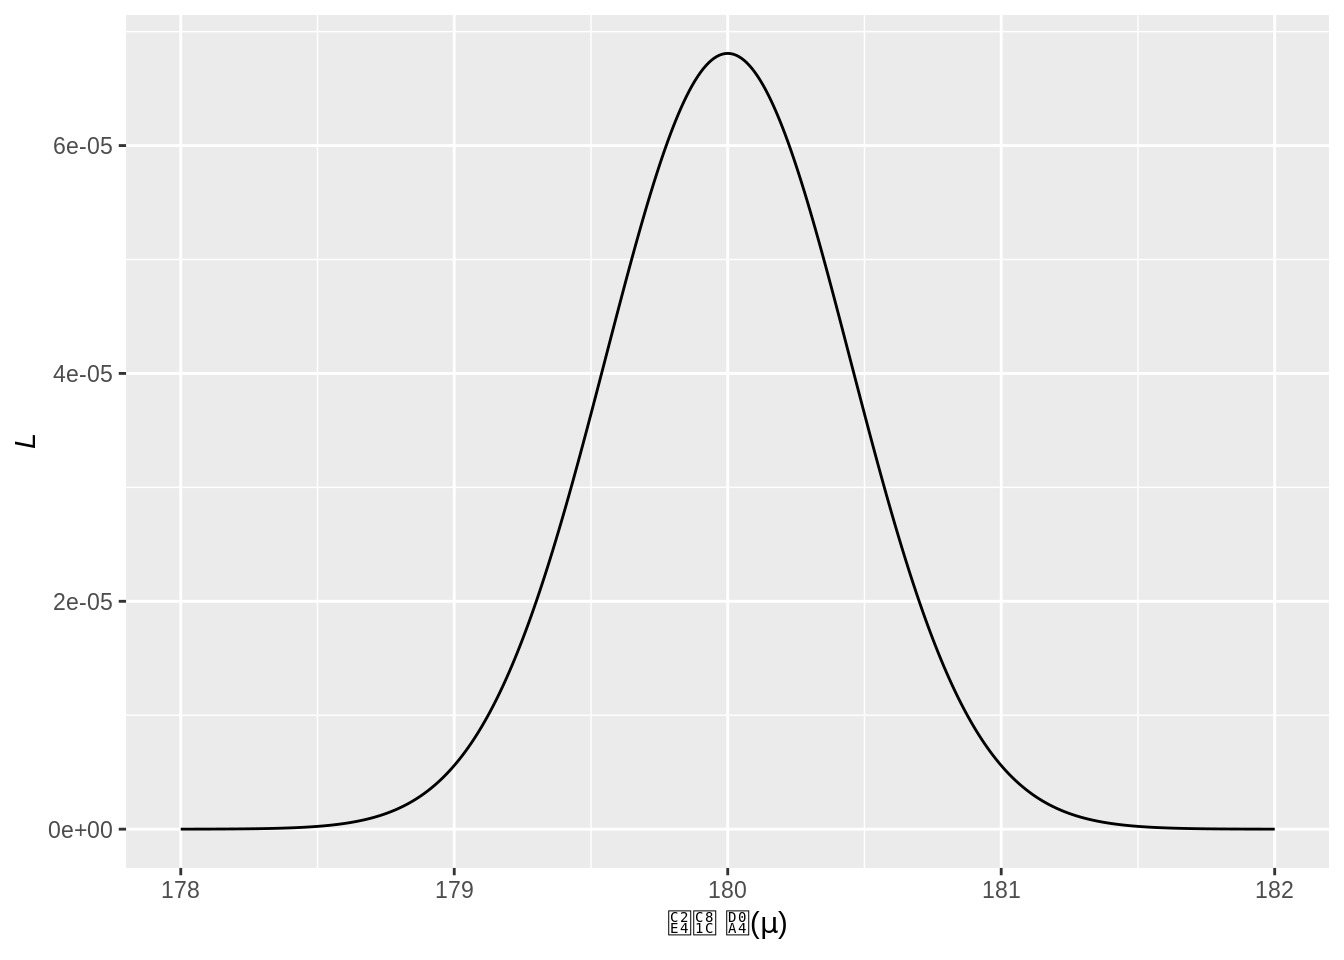
\includegraphics{Basic-stat_files/figure-latex/unnamed-chunk-6-1} 

}

\caption{실제 키에 따른 가능도 $L$의 값}\label{fig:unnamed-chunk-6}
\end{figure}

그림에서도 \(\mu\)가 180일 때 \(L\)의 값이 가장 큰 것을 쉽게 확인할 수 있으며, 앞서 일그러진 동전 때와 마찬가지로 실제 값은 측정값의 평균 정도일 것이라는 우리의 직관과 실제로 계산한 MLE값이 일치하는 것으로 나타났다.

\hypertarget{uxb9c8uxce58uxba70}{%
\section{마치며}\label{uxb9c8uxce58uxba70}}

본 챕터에서는 통계학에서 필수적인 개념인 가능도와 MLE를 이해하기 위해 확률과의 비료를 통해 가능도와 MLE의 개념을 순서대로 설명하였으며, 각 순서마다 이산사건(셀 수 있는 사건)과 연속사건의 2가지 예를 제시하였다. 다음 챕터에서는 정규분포부터 시작해서 최소한으로 꼭 알아야 할 분포를 이야기 할 예정이며, 실제 키의 MLE를 구하는 과정이 거꾸로 적용될 것이니 잘 기억하도록 하자.

\hypertarget{uxc815uxaddcuxbd84uxd3ecnormal-distribution}{%
\chapter{정규분포(Normal distribution)}\label{uxc815uxaddcuxbd84uxd3ecnormal-distribution}}

\hypertarget{uxc2dcuxc791uxd558uxba74uxc11c-1}{%
\section{시작하면서}\label{uxc2dcuxc791uxd558uxba74uxc11c-1}}

이번 단원부터는 통계학에서 중요한 몇 가지 분포를 다루려고 하며, 가장 기본이 되는 \textbf{정규분포}부터 시작하겠다. 앞 단원에서 우리는 키의 측정값이 정규분포를 따른다고 가정했었는데 이렇게 마음대로 가정해도 되는 것인지 의문이 들지 않는가? 그런데 앞으로 통계 분석을 직접 하다 보면 대부분의 연속된 값을 갖는 수치에 대해 정규분포를 가정하는 모습을 보게 될 것이며 실제로 키, 몸무게, 시험 점수 등 대다수의 측정값은 정규분포를 따른다. 실전에서는 심지어 일단 정규분포라고 가정한 다음 도저히 말이 안될 때만 어쩔 수 없이 정규분포 가정을 포기하는 정도이다. 무엇이 정규분포에게 이런 막강한 지위를 부여했을까? \textbf{이항분포(Binomial distribution)의 근사, 오차의 법칙, 중심극한정리}를 통해 막강한 지위의 원천을 하나씩 알아보도록 하자.

\hypertarget{uxc774uxd56duxbd84uxd3ecuxc758-uxadfcuxc0ac}{%
\section{이항분포의 근사}\label{uxc774uxd56duxbd84uxd3ecuxc758-uxadfcuxc0ac}}

우선 이항분포가 무엇인지 간략하게 언급하고 넘어가도록 하겠다. 어렵게 생각할 것 없이 앞단원의 동전던지기를 생각하면 되는데, 동전을 10번 던졌을 때 앞면이 0번 나올 확률부터 10번 나올 확률까지 나열하면 그것이 확률 0.5, 시행횟수 10인 이항분포이다. 주사위를 100번 던져서 1이 0번 나올 확률부터 100번 나올 확률까지 나열하면 바로 확률 \(\frac{1}{6}\), 시행횟수 100인 이항분포가 되며, 일반적으로 \textbf{확률 \(p\)인 사건을 \(N\)번 시행하여 사건 발생 횟수에 따른 확률들을 구하면 그것을 확률 \(p\), 시행횟수 \(N\)인 이항분포라 정의하고 \(B(N,p)\)}로 표현하며 평균은 \(Np\), 분산은 \(Np(1-p)\)임이 잘 알려져 있다. 이렇게 동전던지기와 주사위 던지기를 설명하는 이항분포는 우리 주변의 온갖 사건들을 설명하는 분포인 것 같다. 타율 3할인 타자가 100번 타석에 들어서면 안타를 얼마나 칠 것인가? 어떤 감염병에 걸리면 사망률이 30\%일 때 실제 사람이 얼마나 죽을 것인가? 수능문제 5지선다형을 다 찍으면 몇 점이나 나올 것인가? 등 확률과 발생 정도를 말하는 우리 주변 대부분의 일들은 이항분포를 따른다고 할 수 있으며, 따라서 정규분포가 이항분포의 근사값으로 표현된다면 정규분포 또한 세상의 많은 일들을 설명할 수 있는 분포일 것이다. 그러면 이제부터 이항분포에서 어떻게 정규분포의 이야기가 나오는지 동전과 주사위의 예시를 통해 알아보겠다.

\hypertarget{uxb3d9uxc804uxacfc-uxc8fcuxc0acuxc704uxb97c-uxbb34uxd55cuxd788-uxb358uxc9c0uxba74}{%
\subsection{동전과 주사위를 무한히 던지면?}\label{uxb3d9uxc804uxacfc-uxc8fcuxc0acuxc704uxb97c-uxbb34uxd55cuxd788-uxb358uxc9c0uxba74}}

앞단원에서 동전 10번을 던졌을 때 앞면이 나오는 횟수와 그에 대한 확률을 구하여 그래프로 표현했었다. 그런데 눈치 빠른 사람은 느꼈겠지만 그 그래프는 정규분포의 그것과 모양이 매우 유사한 것을 알 수 있다. 이것은 과연 우연일까?
동전 던지는 횟수를 늘려가며 살펴보도록 하자(앞으로 평균 \(\mu\), 분산이 \(\sigma^2\)인 정규분포를 \(N(\mu,\sigma^2)\)으로 표현하겠다).

\begin{figure}

{\centering 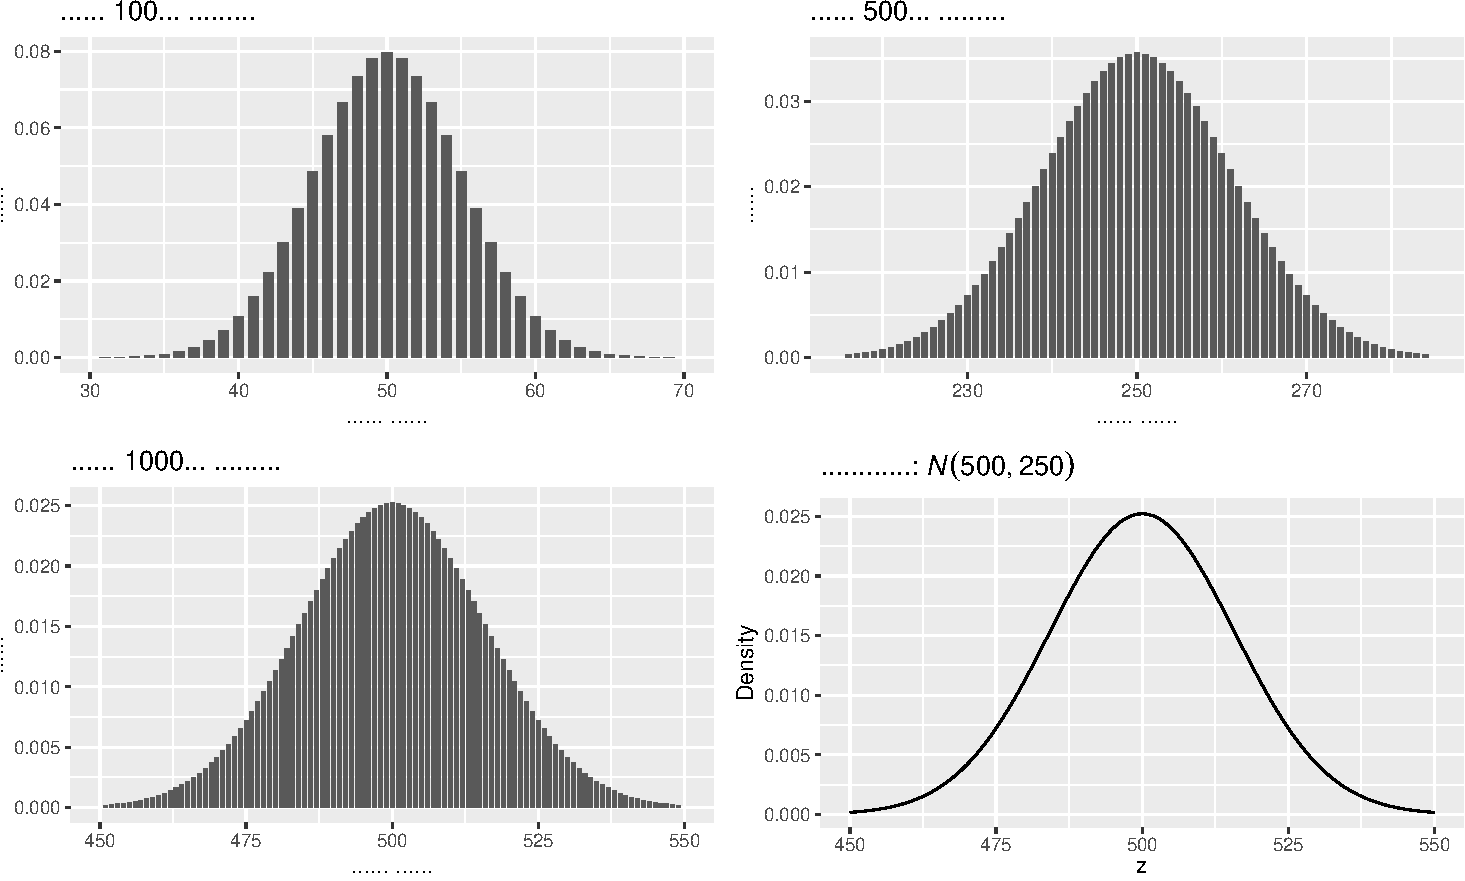
\includegraphics{Basic-stat_files/figure-latex/unnamed-chunk-8-1} 

}

\caption{ 이항분포 VS 정규분포: 동전 던지기}\label{fig:unnamed-chunk-8}
\end{figure}

그래프를 보면 동전을 100번만 던져도 정규분포의 모양과 별로 차이가 없는 것을 알 수 있으며, 1000번을 던졌을 때의 그래프 모양은 평균이 500이고 분산이 250인 정규분포 \(N(500,250)\)과 거의 일치한다. 그러나 혹자는 이 결과에 의문을 가질 것이라 생각하는데, 동전던지기는 50:50의 확률이므로 100번 던져서 앞면이 40번 나올 확률과 60번 나올 확률은 같을 수밖에 없어 그래프의 모양이 좌우대칭일 수 밖에 없다. 그런데 정규분포의 그림도 좌우대칭인 그래프이므로 좌우대칭 효과에 의해 두 그림이 비슷한 것처럼 착시 효과를 보일 수 있다고 생각할 수도 있지 않겠는가? 이런 의문에 답변하기 위해 하나의 예를 더 들어 보겠다. 이번엔 주사위를 여러 번 던져서 1이 나오는 횟수를 구해보자. 1이 나올 확률은 \(\frac{1}{6}\)로 아까 동전던지기 처럼 50:50의 확률이 아니므로 그래프는 분명 좌우 대칭이 아닐 것이고, 그러면 당연히 정규분포와 닮은 그림은 될 수 없을 것이라는 생각이 들지 않는가? 주사위 던지는 횟수를 늘려가면서 살펴보면 아래 그림과 같다.

\begin{figure}

{\centering 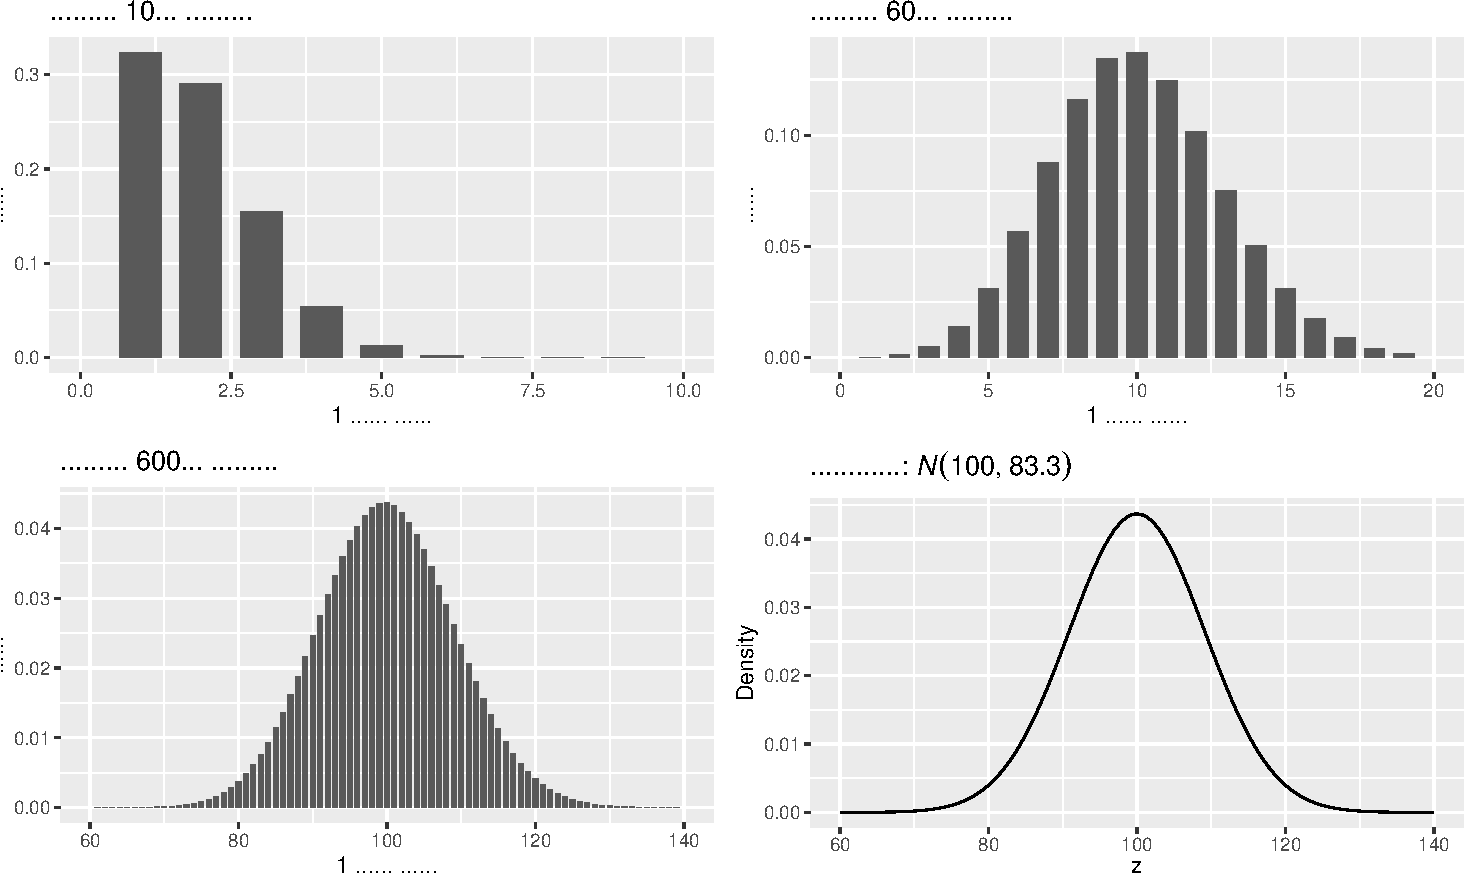
\includegraphics{Basic-stat_files/figure-latex/unnamed-chunk-9-1} 

}

\caption{ 이항분포 VS 정규분포: 주사위 던지기}\label{fig:unnamed-chunk-9}
\end{figure}

어떤가? 주사위를 10번 던졌을 때는 정규분포와는 다른 그래프 모양을 확인할 수 있었으며 좌우대칭의 느낌도 전혀 없다. 10번 던져서 1이 다섯번 이상 나올 확률은 거의 없으며, 1이 한, 두번 나올 확률이 가장 높은 왼쪽으로 치우친 그래프이다. 그러나 60번만 던져도 신기하게 정규분포와 비슷한 모양을 띄기 시작하는 것을 볼 수 있다. 물론 아직까지는 좌우대칭이 아닌 것이 느껴지기는 한다. 600번 정도를 던지게 되면 그래프가 좌우대칭이 아닌 것을 알아차리기 어려우며 정규분포의 모양과 구별을 할 수 없다. 즉, 주사위를 600번 던졌을 때 1이 나오는 횟수를 표현한 그래프는 \(N(100,83.3)\)와 거의 일치한다고 할 수 있다.

\hypertarget{uxc77cuxbc18uxd654}{%
\subsection{일반화}\label{uxc77cuxbc18uxd654}}

동전과 주사위의 예를 간략히 정리해보고 그 결론을 조금씩 일반화해보자. 먼저 이항분포와 정규분포의 표현으로 두 예를 기술하면

\begin{enumerate}
\def\labelenumi{\arabic{enumi}.}
\tightlist
\item
  \(B(1000,0.5)\)는 \(N(1000\times 0.5, 1000\times 0.5 \times 0.5)\) 와 거의 같다.
\item
  \(B(600,\frac{1}{6})\)는 \(N(600\times \frac{1}{6}, 600\times \frac{1}{6} \times \frac{5}{6})\)와 거의 같다.
\end{enumerate}

가 된다(\(600\times \frac{1}{6} \times \frac{5}{6}=83.3\)). 시행횟수가 더 커지면 더 정규분포에 가까워 질 것이라는 것이 우리의 예상이므로 이를 표현하면 다음과 같다.

\begin{enumerate}
\def\labelenumi{\arabic{enumi}.}
\tightlist
\item
  시행횟수 \(N\)이 커질 때, \(B(N,0.5)\)는 \(N(N \times 0.5, N \times 0.5 \times 0.5)\)와 거의 같아진다.
\item
  시행횟수 \(N\)이 커질 때, \(B(N,\frac{1}{6})\)는 \(N(N \times \frac{1}{6}, N \times \frac{1}{6} \times \frac{5}{6})\)와 거의 같아진다.
\end{enumerate}

두 예상을 종합하면 우리는 어떤 추측을 할 수 있을까? 확률을 \(p\)로 바꿔놓고 보면 다음과 같이 두 예상은 하나로 합쳐지게 된다.

\begin{itemize}
\tightlist
\item
  시행횟수 \(N\)이 커질 때, \(B(N,p)\)는 \(N(Np, Npq)\)와 거의 같아진다.
\end{itemize}

그런데 이것은 드무아브르-라플라스의 정리라는 이름으로 이미 수학적으로 증명 되어 있는 내용이다.
따라서 우리는 시행횟수 \(N\)이 커진다면 확률 \(p\)인 사건을 \(N\)번 시행하는 이항분포가 평균 \(Np\), 분산 \(Npq\)인 정규분포와 거의 같아짐을 알 수 있으며, 따라서 정규분포 또한 이항분포와 마찬가지로 세상의 수많은 일들을 설명할 수 있는 분포임을 예상할 수 있다.

\hypertarget{uxc624uxcc28uxc758-uxbc95uxce59-uxc624uxcc28uxb77cuxba74-uxb9c8uxb545uxd788-uxac00uxc9c0uxace0-uxc788uxc5b4uxc57c-uxd560-uxc870uxac74uxb4e4.}{%
\section{오차의 법칙: 오차라면 마땅히 가지고 있어야 할 조건들.}\label{uxc624uxcc28uxc758-uxbc95uxce59-uxc624uxcc28uxb77cuxba74-uxb9c8uxb545uxd788-uxac00uxc9c0uxace0-uxc788uxc5b4uxc57c-uxd560-uxc870uxac74uxb4e4.}}

이번에는 수학자 가우스(Gauss)가 정규분포를 유도한 방법을 알아보도록 하자. 가우스는 이항분포에서 정규분포를 유도하는 방법과는 별개로 오차에 대한 고찰을 통해 정규분포를 유도하였는데, 여기서는 앞단원의 \texttt{나의\ 실제\ 키} 예제와의 비교를 통해 설명하도록 하겠다. \texttt{나의\ 실제\ 키} 예제의 핵심을 간단히 말하면 \textbf{정규분포를 인정한다면, 측정값의 평균을 실제값이라 여기는 우리의 직관은 옳다}는 것이며 좀 더 정확히 표현하면 다음과 같다.

\begin{enumerate}
\def\labelenumi{\arabic{enumi}.}
\tightlist
\item
  키의 측정값 \(x\)이 실제 키의 값인 \(\mu\)를 평균으로 하는 정규분포를 따른다면 즉, \textbf{오차(error) \(\epsilon=x-\mu\)가 평균 0인 정규분포를 따른다면}
\item
  실제 키 \(\mu\) MLE, 즉 \textbf{실제 키일 가능성이 가장 높은 값은 측정값의 평균}이다.
\end{enumerate}

가우스의 논리는 이것을 뒤짚으면 된다. 즉, \textbf{측정값의 평균을 실제값이라 여기는 우리의 직관이 옳다면, 오차는 정규분포를 따른다}는 것이며 좀 더 풀어서 쓰면 다음과 같다.

\begin{enumerate}
\def\labelenumi{\arabic{enumi}.}
\tightlist
\item
  실제 키의 MLE, 즉 실제 키일 가능성이 가장 높은 값은 측정값의 평균이라면
\item
  오차는 정규분포를 따른다.
\end{enumerate}

가우스는 여기에 오차라면 마땅히 가져야 할 조건 3개를 추가하여 다음과 같은 \textbf{오차의 법칙}을 제시하였다.

\begin{enumerate}
\def\labelenumi{\arabic{enumi}.}
\tightlist
\item
  +오차와 -오차가 나올 가능성은 같다. 즉, 오차의 분포를 나타내는 확률밀도 함수 \(f\)는 \(f(-\epsilon)=f(\epsilon)\)인 좌우대칭 함수이다.\\
\item
  작은 오차가 나올 가능성이 큰 오차가 나올 가능성보다 크다. 즉, \(f(\epsilon)\)는 위로 볼록한 모양이다.
\item
  \(f(\epsilon)\)는 2번 미분가능하고, 전체 확률은 1이다. 즉, \(\int_{-\infty}^{\infty} f(\epsilon) d\epsilon=1\)
\item
  참값의 MLE는 측정값의 평균값이다. 즉, \(n\)번 측정하여 측정값을 각각 \(x_1, x_2, \cdots, x_n\)이라 할 때 가능도 \(L=f(x_1-\mu)f(x_2-\mu)\dots f(x_n-\mu)\)는 \(\mu=\frac{x_1+x_2+\cdots+x_n}{n}\)에서 최대값을 갖는다.
\end{enumerate}

조건 1,2,3는 직관적으로 오차의 성질로 받아들일 수 있는 조건들로 이들을 포함한 총 4개의 조건에서 정규분포의 확률밀도함수(PDF)를 직접 수학적으로 유도할 수 있고, 결국 정규분포가 세상의 온갖 측정값을 설명하는 중요한 분포라는 결론에 이르게 된다. 혹시 유도 과정이 궁금한 독자는 \url{http://wiki.mathnt.net/index.php?title=정규분포와_그_확률밀도함수} 를 참고하기 바란다.

\hypertarget{uxc911uxc2ecuxadf9uxd55cuxc815uxb9ac-uxbb34uxc870uxac74-uxc815uxaddcuxbd84uxd3ec-ok}{%
\section{중심극한정리: 무조건 정규분포 OK?}\label{uxc911uxc2ecuxadf9uxd55cuxc815uxb9ac-uxbb34uxc870uxac74-uxc815uxaddcuxbd84uxd3ec-ok}}

나를 포함한 많은 사람들은 평균을 참 좋아한다. 시험성적 평균 60점, 대한민국 평균수명은 80살, 1인당 평균 국민소득은 2만6천달러 등 집단을 평가, 비교하는데 가장 흔히 쓰이는 지표가 평균이며 이제부터 할 이야기의 핵심 지표가 바로 \textbf{표본평균(Sample mean)}이다. 우리는 흔히 모집단에서 표본을 뽑아 그것의 평균을 계산한 표본평균값을 전체의 평균값이라 여기곤 하는데 이것의 대표적인 예가 여론조사이다. 고작 수백명을 무작위로 뽑아 여론조사를 해서 특정 안건에 대한 찬성률을 계산한 후, 이것을 전체 민심의 척도로 간주하는 것은 일리있다고 할 수 있을까? 우선 앞에서 다루었던 찌그러진 동전과 주사위 던지기의 예를 통해 알아보도록 하자.

\hypertarget{uxcc0cuxadf8uxb7ecuxc9c4-uxb3d9uxc804-uxb358uxc9c0uxae30.}{%
\subsection{찌그러진 동전 던지기.}\label{uxcc0cuxadf8uxb7ecuxc9c4-uxb3d9uxc804-uxb358uxc9c0uxae30.}}

앞단원에서 다루었던 찌그러진 동전을 다시 생각해 보자. 이 동전은 모양이 찌그러져서 앞면이 나올 확률 \(p\)가 0.5가 아닌 0.4였으며, 앞면이 나오는 사건을 1, 뒷면이 나오는 경우를 0이라 하면 분산은 \(p \times (1-p)^2 + (1-p) \times (0-p)^2 = p(1-p) = 0.24\)이다.

이제 직접 동전을 여러 번 던져서 앞면이 나올 확률을 계산한 후, 실제 확률인 0.4와 얼마가 차이가 나는지 알아볼 것인데 그 과정은 다음과 같다.

\begin{enumerate}
\def\labelenumi{\arabic{enumi}.}
\tightlist
\item
  앞면이 나올 확률을 얻기 위해 수행한 동전 던지기 횟수, 즉 표본수를 \(n\)이라 하자.
\item
  \(n=10\)일 때 앞면이 나올 확률 \(\hat{p}\)을 계산한다.
\item
  2의 과정을 10000번 반복하여 10000개의 \(\hat{p}\)를 얻는다. 꼭 10000개일 필요는 없으며 \(\hat{p}\)의 분포를 파악할 수 있을 정도면 된다.
\item
  \(\hat{p}\)들의 분포를 그래프로 그려보고 그것들의 평균, 분산을 구해본다.
\item
  \(n=30, 100\)인 경우에도 마찬가지 과정을 수행한다.
\end{enumerate}

\begin{figure}

{\centering 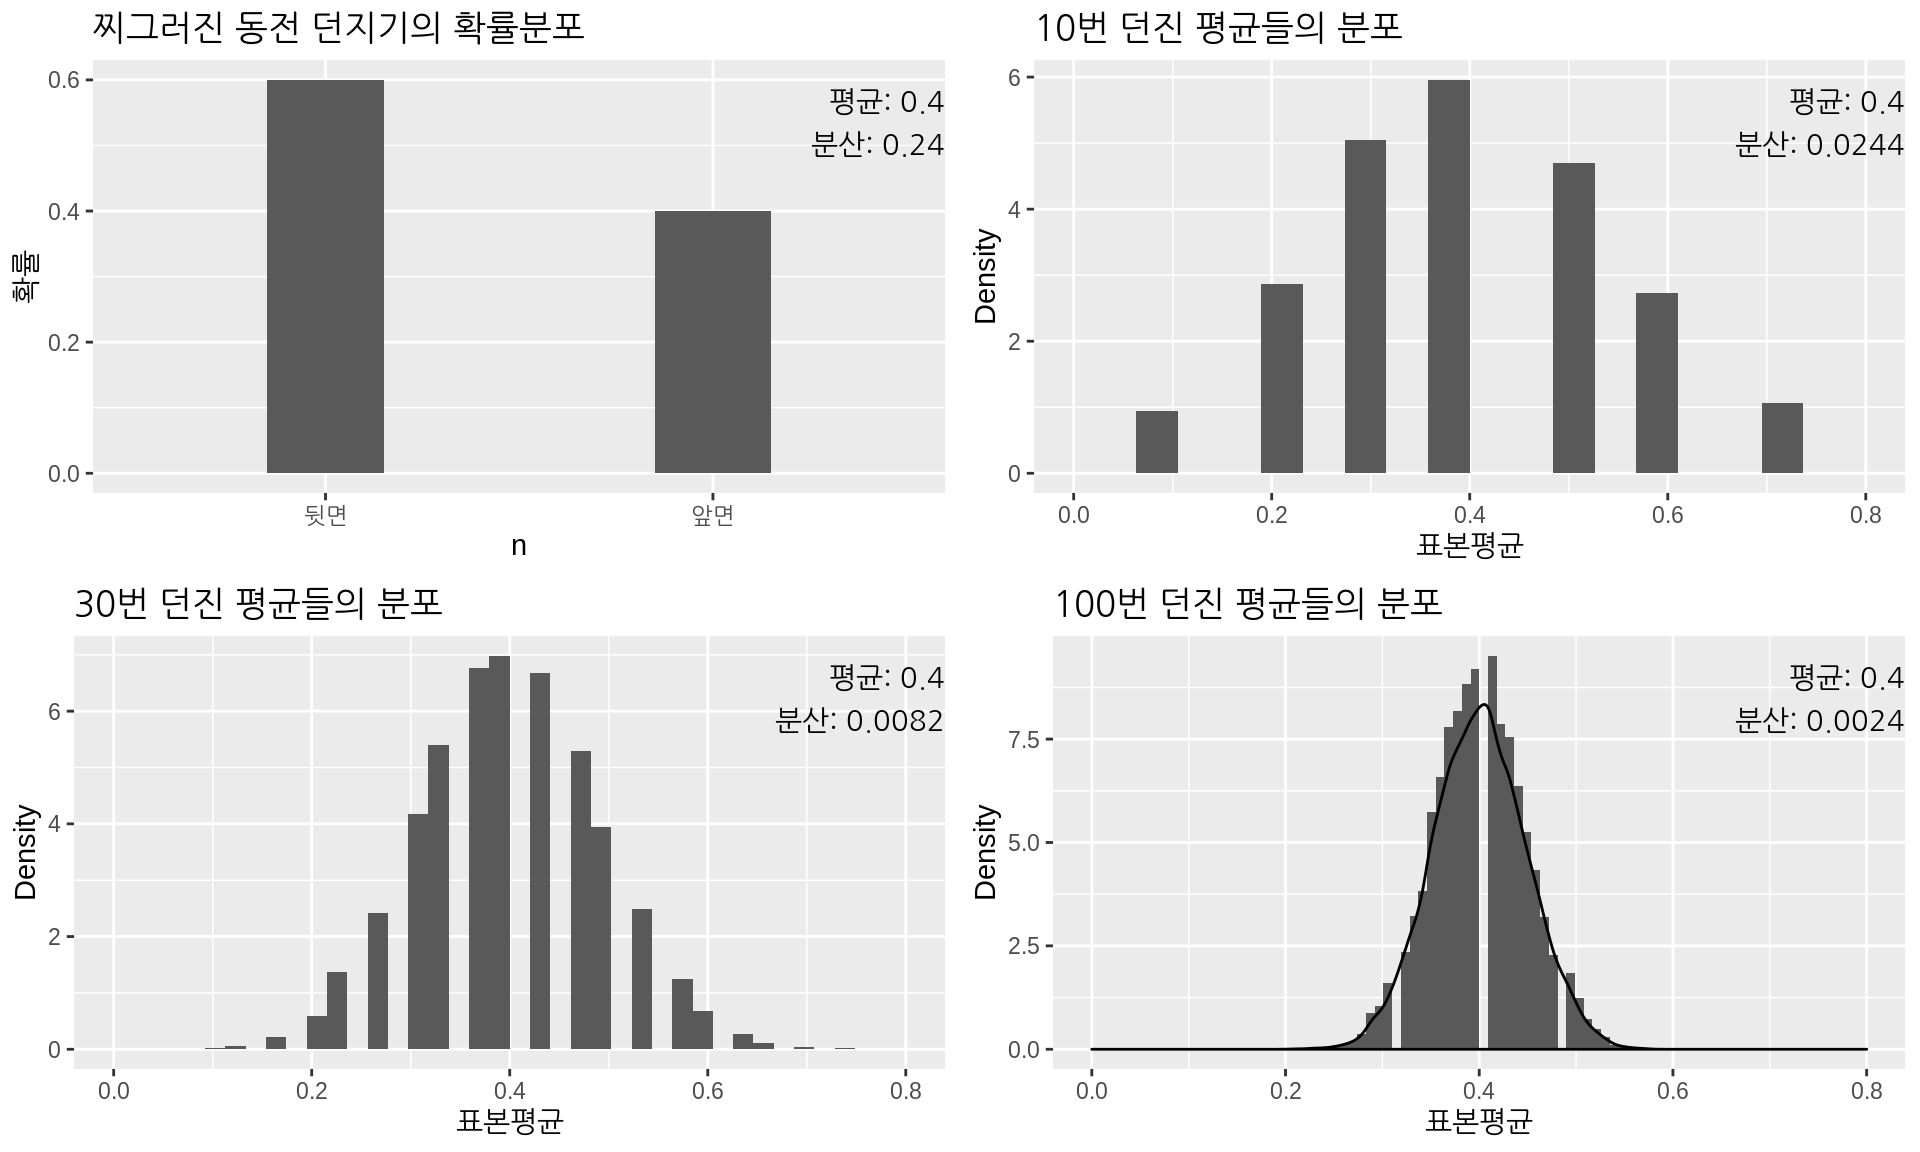
\includegraphics{Basic-stat_files/figure-latex/unnamed-chunk-10-1} 

}

\caption{확률분포 & 표본평균분포: 찌그러진 동전 던지기}\label{fig:unnamed-chunk-10}
\end{figure}

그림을 보면 아래와 같은 몇 가지의 규칙을 발견할 수 있다.

\begin{enumerate}
\def\labelenumi{\arabic{enumi}.}
\tightlist
\item
  \(n\)이 증가할수록, 특히 30 이상부터는 \(\hat{p}\)의 분포는 정규분포와 비슷해진다.
\item
  \(\hat{p}\)의 평균은 실제 \(p\)값인 0.4와 가까워진다.
\item
  \(\hat{p}\)의 분산은 실제 앞면이 나오는 사건의 분산을 \(n\)으로 나눈 값인 \(\frac{0.24}{n}=\frac{p(1-p)}{n}\)과 가까워진다.
\end{enumerate}

이제 이것들을 종합하면 \textbf{\(n\)이 커지면 \(\hat{p}\)는 평균이 \(p\)이고 분산이 \(\frac{p(1-p)}{n}\)인 정규분포, 즉 \(N(p,\frac{p(1-p)}{n})\)을 따른다}는 추측을 할 수 있다.

\hypertarget{uxc8fcuxc0acuxc704uxb97c-uxb358uxc838uxc11c-uxb098uxc624uxb294-uxc22buxc790uxc758-uxd3c9uxade0uxac12.}{%
\subsection{주사위를 던져서 나오는 숫자의 평균값.}\label{uxc8fcuxc0acuxc704uxb97c-uxb358uxc838uxc11c-uxb098uxc624uxb294-uxc22buxc790uxc758-uxd3c9uxade0uxac12.}}

이번에는 다시 주사위 이야기로 돌아가서 주사위를 던졌을 때 평균적으로 얼마가 나올 것인지 생각해 보자. 1,2,3,4,5,6
중 랜덤으로 하나가 나올 것이므로 평균(\(\mu\))은 \(\frac{1+2+3+4+5+6}{6}=3.5\)가 되고 분산(\(\sigma^2\))을 구해보면 \(\frac{(1-3.5)^2+(2-3.5)^2+\cdots+(6-3.5)^2}{6}\approx 2.92\)가 된다. 이제 동전던지기 때와 마찬가지로 아래의 시행을 통해 표본평균(\(\bar{X}\))과 실제 평균(\(\mu\))을 비교해 보겠다.
아

\begin{figure}

{\centering 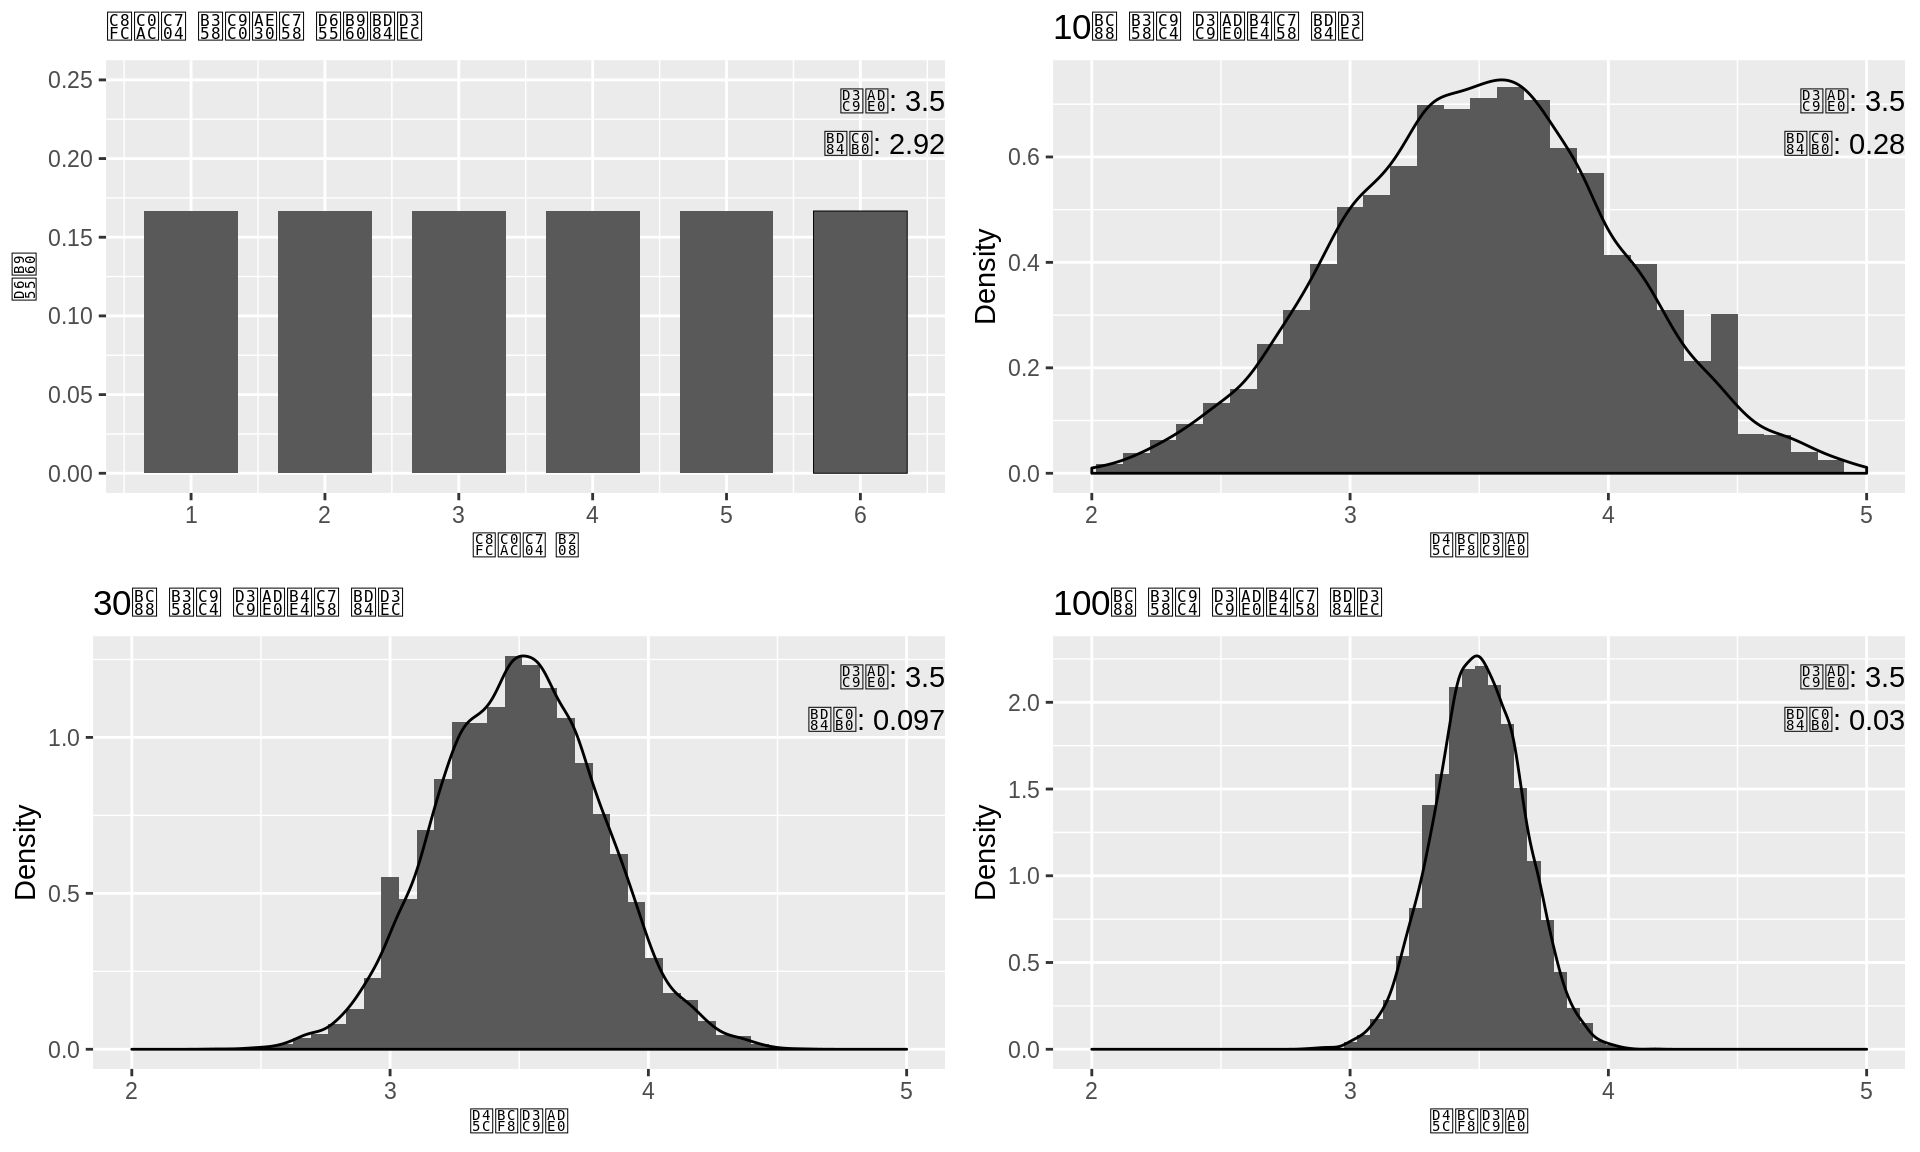
\includegraphics{Basic-stat_files/figure-latex/unnamed-chunk-11-1} 

}

\caption{확률분포 & 표본평균분포: 주사위 던지기}\label{fig:unnamed-chunk-11}
\end{figure}

그림을 보면 동전던지기 때와 유사하다는 느낌을 받을 수 있는데 아래와 같이 결과를 정리해보면 더욱 확실해진다.

\begin{enumerate}
\def\labelenumi{\arabic{enumi}.}
\tightlist
\item
  \(n\)이 증가할수록, 특히 30 이상부터는 표본평균 \(\bar{X}\)의 분포는 정규분포와 유사해진다.
\item
  \(\bar{X}\)의 평균은 실제 평균인 \(\mu=3.5\)에 가까워진다.
\item
  \(\bar{X}\)의 분산은 \(\frac{2.92}{n}=\frac{\sigma^2}{n}\)에 가까워진다.
\end{enumerate}

따라서 이것들을 종합하면 동전던지기 때와 비슷하게 \textbf{\(n\)이 커지면 \(\bar{X}\)는 평균이 \(\mu\)이고 분산이 \(\frac{\sigma^2}{n}\)인 정규분포, 즉 \(N(\mu,\frac{\sigma^2}{n})\)을 따른다}는 추측을 할 수 있다.

이쯤되면 확률분포의 종류에 상관없이 \(n\)이 커지면 표본평균 \(\bar{X}\)는 평균이 \(\mu\)이고 분산이 \(\frac{\sigma^2}{n}\)인 정규분포를 따르지 않을까? 라는 과감한 추측을 할 수도 있을 것 같다. 그러나 동전던지기나 주사위 던지기는 둘 다 사건의 갯수가 유한한 이산확률분포로 일반화하기에는 무리가 있어, 연속확률분포에 대해서도 실험을 해 봐야 할 것 같다. 정규분포를 비롯한 몇 가지 예를 통해 연속확률분포의 경우에도 같은 추측을 할 수 있을지 알아보도록 하자.

\hypertarget{uxd45cuxc900uxc815uxaddcuxbd84uxd3ecuxc5d0uxc11c-uxc22buxc790-uxbf51uxae30}{%
\subsection{표준정규분포에서 숫자 뽑기}\label{uxd45cuxc900uxc815uxaddcuxbd84uxd3ecuxc5d0uxc11c-uxc22buxc790-uxbf51uxae30}}

이번에는 가장 기본적인 연속확률분포인 표준정규분포(\(\mu=0\), \(\sigma^2=1\))에서 \(n\)개의 숫자를 뽑아 평균을 내는 경우를 살펴보자. 과정은 앞서 동전, 주사위 던지기와 유사하므로 설명은 생략하고 바로 그림을 살펴보자.

\begin{figure}

{\centering 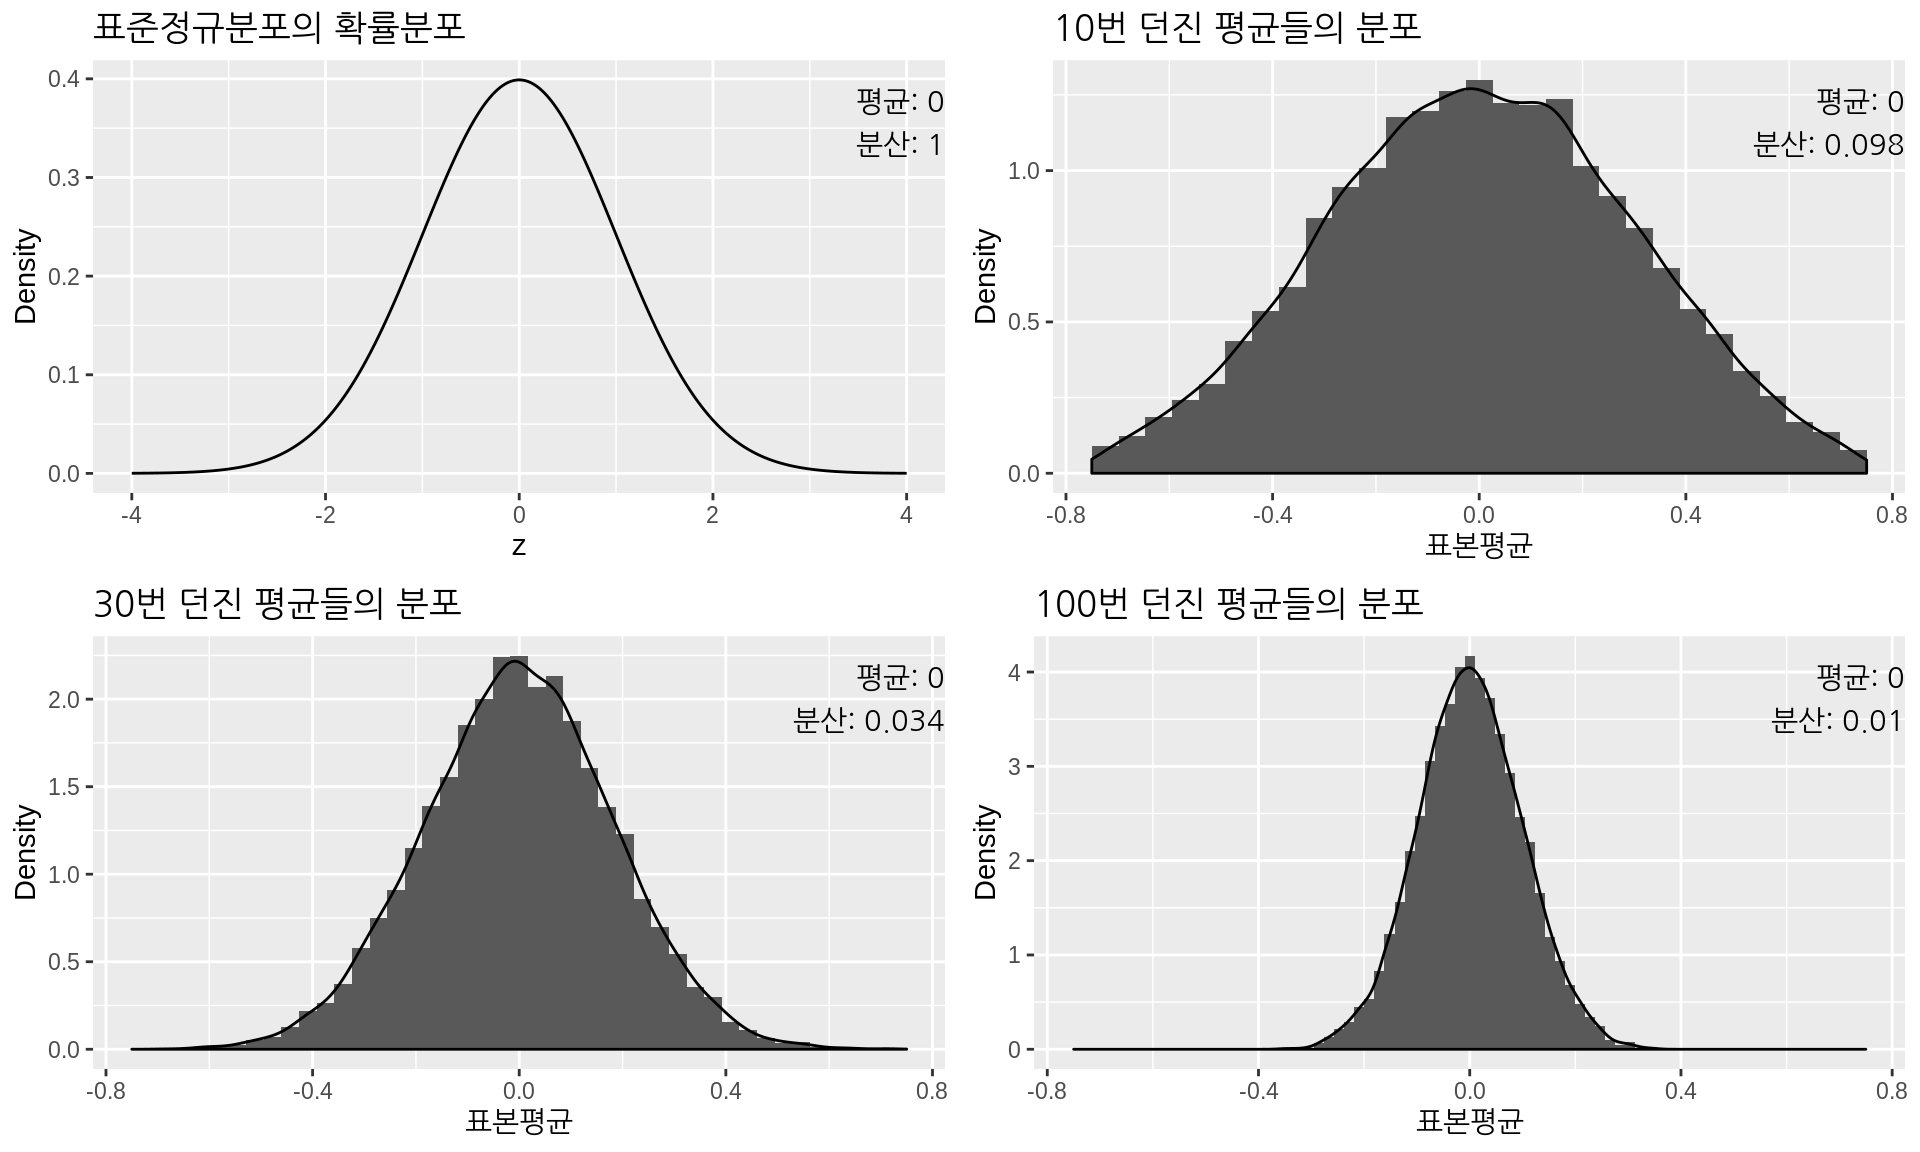
\includegraphics{Basic-stat_files/figure-latex/unnamed-chunk-12-1} 

}

\caption{확률분포 & 표본평균분포: 표준정규분포}\label{fig:unnamed-chunk-12}
\end{figure}

어떤가? 이번에도 역시 \(n=30\)만 되어도 표본평균 \(\bar{X}\)가 정규분포를 따르는 것을 느낄 수 있으며, \(\bar{X}\)의 평균은 실제 평균 0에, 분산은 \(\frac{1}{n}\)에 가까워졌고, 이제는 진짜 모든 경우에 우리의 추측이 성립하는 것 같다. 그래도 혹시나 하는 마음에 정규분포가 아닌 연속확률분포에서의 예제를 마지막으로 다루어 보겠다.

\hypertarget{uxce74uxc774uxc81cuxacf1uxbd84uxd3ecchi-square-distribution}{%
\subsection{카이제곱분포(Chi-square distribution)}\label{uxce74uxc774uxc81cuxacf1uxbd84uxd3ecchi-square-distribution}}

카이제곱분포에 대한 자세한 설명은 다음 단원에서 다룰 예정이므로, 여기서는 자유도가 1인 카이제곱분포가 정규분포와는 달리 왼쪽으로 치우친 분포이며 평균 \(\mu=1\), 분산 \(\sigma^2=2\)라는 것만 알고 바로 앞의 과정을 진행하겠다.

\begin{figure}

{\centering 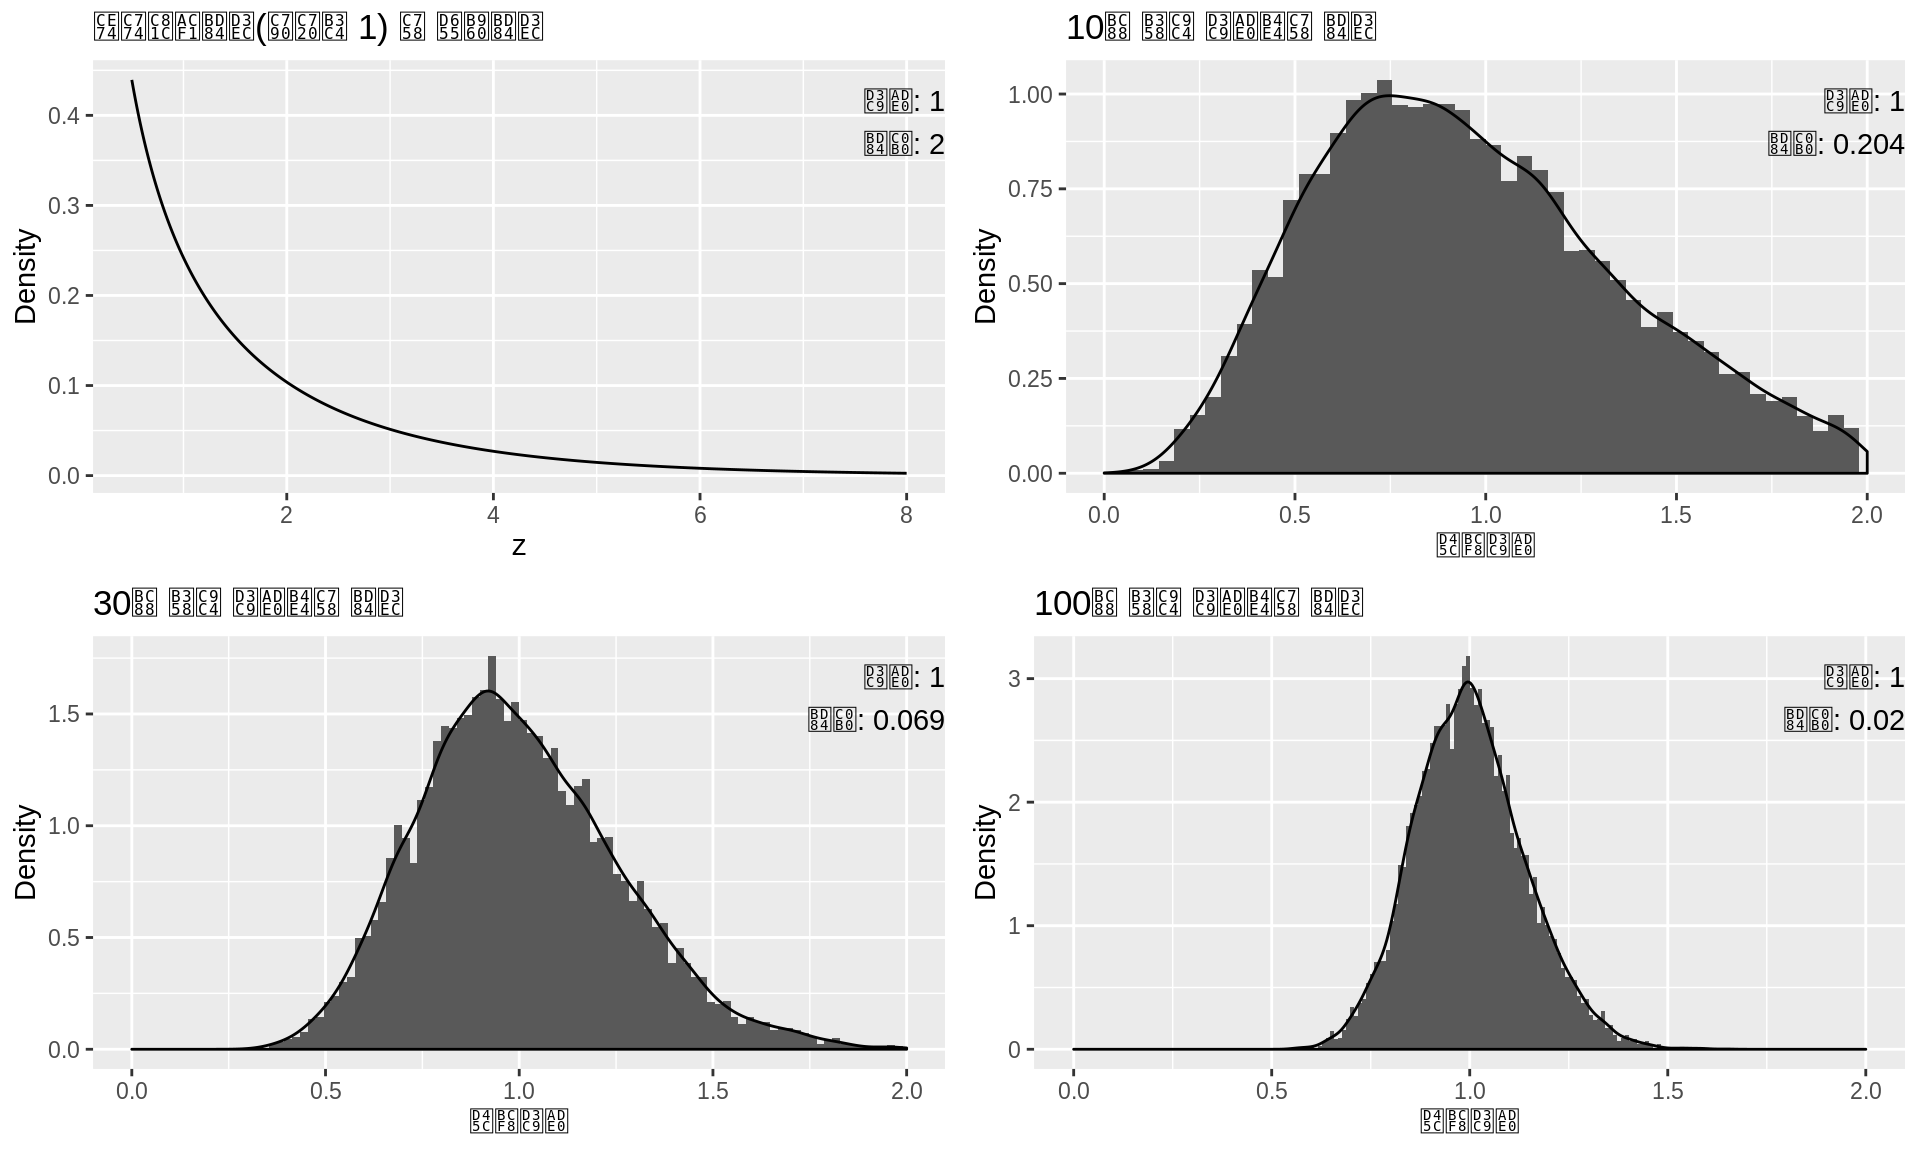
\includegraphics{Basic-stat_files/figure-latex/unnamed-chunk-13-1} 

}

\caption{확률분포 & 표본평균분포: 카이제곱분포(자유도 1)}\label{fig:unnamed-chunk-13}
\end{figure}

그림을 살펴보면 \(n=10\)일 때는 원래 카이제곱 분포만큼은 아니어도 미세하게 왼쪽으로 치우친 느낌이 들지만 \(n=30\)만 되어도 정규분포의 모양을 보임을 확인할 수 있으며, 지금까지와 마찬가지로 표본평균들의 평균은 실제 카이제곱분포의 평균인 1, 분산은 카이제곱 분포의 분산을 표본수로 나눈 \(\frac{2}{n}\)에 가까워지는 것을 확인할 수 있다.

이제 한쪽으로 치우친 연속확률분포의 경우까지 확인했으므로 더 이상 망설이지 않고 외칠 수 있다

\textbf{평균이 \(\mu\), 분산이 \(\sigma^2\)인 모집단에서(정규분포일 필요 없음) \(n\)개의 표본을 뽑아서 계산한 표본평균 \(\bar{X}\)는 \(n\)이 커질 때 \(N(\mu,\frac{\sigma^2}{n})\)을 따른다.}

이것이 바로 통계학에서 가장 중요하다고 일컬어지는 \textbf{중심극한정리(Central Limit Theorem, CLT)}이며 이미 수학적으로 증명이 되어 있다. 이제 정규분포가 얼마나 중요한 분포인지 느껴지는가? 모집단이 어떻게 생겼든 상관없이 30개 표본정도만 확보하면 표본평균들은 무조건 정규분포를 따른다고 우겨도 괜찮다는 뜻이다.

이제 우리는 정규분포가 세상에서 가장 중요한 분포인 이유를 3가지나 알았다. \textbf{이항분포}에서도 만들 수 있고 가장 간단한 \textbf{오차의 법칙}으로부터도 만들 수 있으며 대부분의 \textbf{표본평균을 설명하는 분포}인 정규분포, 사람들이 왠만하면 정규분포만 쓰는 것은 지극히 정상적인 판단이라고 할 수 있다.

\hypertarget{uxc911uxc2ecuxadf9uxd55cuxc815uxb9ac-uxace0uxcc30}{%
\section{중심극한정리 고찰}\label{uxc911uxc2ecuxadf9uxd55cuxc815uxb9ac-uxace0uxcc30}}

앞서 중심극한정리를 통계학에서 가장 중요하다고 말했는데 이런 중요한 내용을 고작(?) 정규분포의 중요성을 설명하는 것에만 활용하는 것은 너무 아쉬운 일이라고 생각한다. 정규분포의 이야기를 제외하더라도 표본평균의 평균과 분산에 대한 이야기가 남아있지 않은가? 이 중 표본평균의 평균이 실제 평균에 가까워질 것은 직관적으로 당연하게 받아들일 수 있는 내용이지만, 분산에 대한 이야기는 그렇지 않다. 표본평균의 분산이 원래 모집단 분산을 \(n\)으로 나눈 \(\frac{\sigma^2}{n}\)이 된다는 것에서 우리는 무엇을 깨달을 수 있을까? 첫째로는 \textbf{쪽수가 깡패(?)}임을 알 수 있다. \(n\)이 계속 커지면 표본평균의 분산은 점점 0에 가까워지게 되어 표본평균을 그냥 실제평균으로 간주해도 문제가 없게 된다. 학생 100명이 수학시험을 보았을 때, 10명을 뽑아 평균을 내는 것보다 50명을 뽑아 평균을 내는 것이 더 정확할 것이라는 지극히 자연스러운 이야기이다. 둘째로는 \textbf{의심의 정도를 숫자로 표현할 수 있다}는 점이며, 앞서 다루었던 찌그러진 동전의 예를 다시 떠올려보자. 우리는 동전이 찌그러져서 앞면이 나올 확률 \(p\)가 0.4인줄로 알고 있다. 그런데 실제 동전을 10번 던졌더니 앞면이 6번 나와서 확률이 0.6으로 계산되어 실제 확률 0.4와 0.2가 차이난다면 이 일을 어떻게 받아들여야 하는가? 아래의 그림을 본 후에 생각해 보자.

\begin{figure}

{\centering 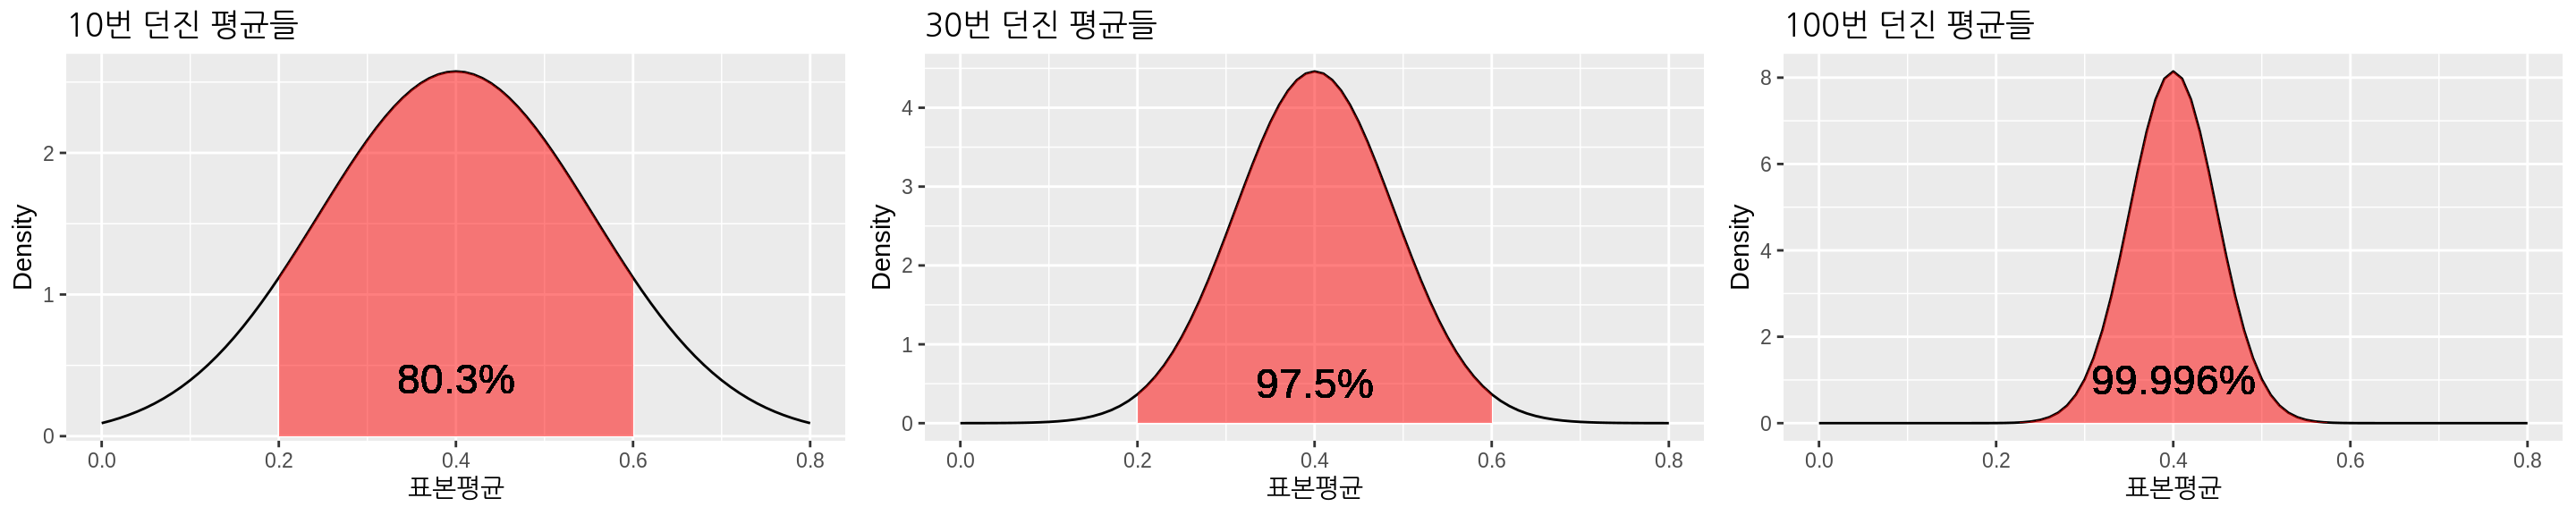
\includegraphics{Basic-stat_files/figure-latex/unnamed-chunk-14-1} 

}

\caption{찌그러진 동전 던지기(중심극한분포 이용한 정규분포 근사)}\label{fig:unnamed-chunk-14}
\end{figure}

동전을 열번 던졌을 때의 그림을 다시 살펴보면 뭐 0.2정도 차이는 날 수도 있겠구나.. 라는 생각이 들 것이다. 실제로 표본확률의 평균의 분포가 \(N(0.4,0.024)\)에 가까워 진다는 중심극한정리를 이용하여 표본확률값이 0.4와 \(\pm 0.2\)이상 차이날 확률을 계산해보면 대략 19.7\% 가 된다. 이 정도면 뭐 일어날 수도 있다고 생각하고 넘어갈 수 있지 않겠는가? 이번에는 확률은 똑같이 0.6이지만 동전을 30번 던져서 앞면이 18번 나온 경우를 생각하자. 그림을 보니 이제는 좀 이상하다. 딱 봐도 실제확률인 0.4와 \(\pm 0.2\)이상 차이가 나는 경우가 별로 없는 것처럼 보이며, 직접 계산을 해봐도 \(\pm 0.2\)이상 차이가 날 가능성은 2.5\% 로 \textbf{5\%도 안된다}. 이쯤되면 원래의 동전상태를 의심해봐야 하는 것 아닐까? 진짜로 동전이 찌그러져서 앞면확률이 0.4라면 어떻게 동전 30번을 던져 앞면이 18번이나 나올 수 있겠는가? 이 정도 이상으로 차이가 날 확률은 2.5\%밖에 안되는데 말이다. 동전을 100번 던져서 앞면이 60번이 나와서 확률 0.6을 얻었다면 이제는 거짓말을 확신할 수 있을 것이다. 동전을 100번 던져서 앞면이 20번 이하 또는 60번 이상 나올 확률은 0.004\% 로 거의 0에 가까운데 누가 앞면이 나올 확률이 0.4라는 말을 믿겠는가? 이처럼 중심극한정리를 이용하면 우리의 의심의 정도를 계량화할 수 있으며, 같은 결과라도 \(n\)수가 얼마나 되는가에 따라 의심하는 정도는 달라지게 된다. 의심 정도를 계량화한다는 개념은 추후 나올 \textbf{\(P\) value}의 개념으로 바로 연결되므로 잊지 않고 기억해주길 바란다.

\hypertarget{uxb9c8uxce58uxba70-1}{%
\section{마치며}\label{uxb9c8uxce58uxba70-1}}

이번 단원에서는 정규분포의 당위성을 뒷받침하는 3가지의 근거를 다양한 예시와 실험을 통해 알아보았으며, 그 중 중심극한정리에 대해서는 따로 그 의미를 되새겨보았다. 다음 단원에서는 정규분포 외에 알아야 하는 확률분포를 딱 3개만 더 알아보도록 하겠으며, 그 후에는 본격적으로 통계분석의 세계로 들어가 보도록 하겠다.


\end{document}
